\documentclass[10pt]{beamer}

\usetheme{CUDenver}

\usepackage{mathtools}
\usepackage[abs]{overpic}
\setlength\unitlength{1mm}

\usepackage{color}
\usepackage{graphicx}
\usepackage{url}
\usepackage{xspace}
\usepackage{tikz}
\usetikzlibrary{arrows,positioning}
\usepackage{subfigure}
\usepackage{verbatim}
\usepackage{amsfonts}
\usepackage{amsmath}
\usepackage{amssymb}
\usepackage{amsbsy}
\usepackage{amsthm}
\usepackage[mathcal]{euscript}
\usepackage{algorithmic}
\usepackage{boxedminipage}
\usepackage{fancyvrb}
\usepackage{epstopdf}
\usepackage[lined,ruled]{algorithm2e}

\newcommand{\tred}[1]{\textcolor{Red}{#1}}
\newcommand{\tgreen}[1]{\textcolor{Green}{#1}}
\newcommand{\tcyan}[1]{\textcolor{Cyan}{#1}}
\newcommand{\tyellow}[1]{\textcolor{Yellow}{#1}}
\newcommand{\tpurple}[1]{\textcolor{Purple}{#1}}
\newcommand{\tblack}[1]{\textcolor{Black}{#1}}
\newcommand{\tgrey}[1]{\textcolor{Grey}{#1}}
\newcommand{\tdeepred}[1]{\textcolor{deepred}{#1}}
\definecolor{Green}{rgb}{0,.5,0}
%use for definitions
\definecolor{Red}{rgb}{.8,.2,0}
%use for emphasis
\definecolor{Yellow}{rgb}{.6,.6,.1}
%use for part titles
\definecolor{Cyan}{rgb}{.2,.6,.7}
%use for comments
\definecolor{Purple}{rgb}{.4,0,1}
%use for examples
\definecolor{deepred}{rgb}{.53,.29,.24}
%use for important points
\definecolor{Black}{rgb}{0,0,0}
%use for washout
\definecolor{Grey}{rgb}{.45,.45,.45}
%%%%%%%%%%%%%%%%%%%%%%%%%%%%%%%%%%%%%%%%%%%%%%%%%%%%%%%%%%%%%%%%%%%%%%%%%%%%%%%%
% newcommands.tex

% itemize with the explaining text left justified afer the item
% Example:
%   \itembox{CNR} The Control net reduction
%   \itembox{A} Another item
% renders as
% * CNR   The Control net reduction
% * A     Another item
\newcommand{\itembox}[1]{\item {\makebox[0.25in]{#1 \hfill}}}

% Abbreviations
\newcommand{\ie}{{\itshape i.e.}}
\newcommand{\eg}{{\itshape e.g.}}

% Bold symbols
\newcommand{\bs}[1]{\boldsymbol{#1}}

% Cardinality
\newcommand{\card}[1]{n\left(#1\right)} %{\left|#1\right|}
\newcommand{\set}[1]{\left\{#1\right\}}
\newcommand{\nullset}{\varnothing}

% Math Operators
\DeclareMathOperator*{\argmin}{arg\,min}
\DeclareMathOperator*{\argmax}{arg\,max}
\newcommand{\abs}[1]{\left\vert#1\right\vert}
\newcommand{\norm}[1]{\left\Vert#1\right\Vert}
\newcommand{\mat}[2]{\left[\begin{array}{#1}#2\\ \end{array}\right]}

% Standard Probability
\DeclareMathOperator{\E}{\mathbb{E}}
% Measure
\newcommand{\PP}{\mathbb{P}}
% Density
\newcommand{\pp}{\pi}
% Space of measures/solutions
\newcommand{\PPspace}{\mathcal{P}}


% indices into sets/spaces
\newcommand{\iparam}{i} % index into parameter space (num samples)
\newcommand{\imesh}{h} % index into mesh/model refinement sequence
\newcommand{\iobs}{k} % index into QoI
\newcommand{\idisc}{k} % index into output discretization
\newcommand{\idata}{j} % index into data (target)

% Sets/Spaces
\newcommand{\RR}{\mathbb{R}}
\renewcommand{\NN}{\mathbb{N}}
\newcommand{\OO}{\mathcal{O}} % sets of indices for set-based inversion alg
\renewcommand{\LL}{\mathcal{L}} % transverse parameterization
\newcommand{\VV}{\mathcal{V}} % voronoi
\newcommand{\BB}{\mathcal{B}} % borel

\newcommand{\CC}{\mathcal{C}} % contour symbol
\newcommand{\cborel}{\CC_{\pspace}} % contour sigma algebra
\DeclareMathOperator*{\contourP}{\PP_{\cborel}}

\DeclareMathOperator*{\paramP}{\PP_{\pspace}}
\DeclareMathOperator*{\dataP}{\PP_{\dspace}}

\newcommand{\nparams}{P}
\newcommand{\RP}{\RR^\nparams} % parameter space dimensions
\newcommand{\nsamps}{N} % num samples

\newcommand{\ndata}{D} % num data points collected for each observable
\newcommand{\RD}{\RR^\ndata} % data space dimensions

% Sample-Based
\newcommand{\nobs}{O} % number of observables
\newcommand{\RO}{\RR^\nobs} % qoi data space dimensions

% Set-Based
\newcommand{\ndiscs}{M} % number of cells used to discretize data space

\newcommand{\sa}{\sigma\text{-algebra}}
\newcommand{\Chi}{\mbox{\LARGE$\chi$}}

\newcommand{\Rho}{\mbox{\LARGE$\rho$}}
\newcommand{\Nu}{\mbox{\Large$\nu$}}

\newcommand{\true}{\dagger}
% Data-Consistent Inversion Framework
\newcommand{\dimP}{P}
\newcommand{\dimD}{D}
\newcommand{\param}{\lambda}
\newcommand{\paramref}{\param^\true}
\newcommand{\pspace}{{\Lambda}}
\newcommand{\pmeas}{\mu_{\pspace}}
\newcommand{\pborel}{\BB_{\pspace}}
\newcommand{\Pspace}{(\pspace, \pborel, \pmeas)}

\DeclareMathOperator*{\initialP}{\PP_{in}}
\DeclareMathOperator*{\initial}{\pp_{in}}
\DeclareMathOperator*{\updatedP}{\PP_{up}}
\DeclareMathOperator*{\updated}{\pp_{up}}

\DeclareMathOperator*{\obs}{\boldsymbol{o}}
\DeclareMathOperator*{\data}{\boldsymbol{d}}
\newcommand{\dspace}{\mathcal{D}}
\newcommand{\dmeas}{\mu_{\dspace}}
\newcommand{\dborel}{\BB_{\dspace}}
\newcommand{\Dspace}{(\dspace, \dborel, \dmeas)}


% Labeled QoI maps
\newcommand{\qoiA}{\qoi^{(a)}}
\newcommand{\qoiB}{\qoi^{(b)}}
\newcommand{\qoiC}{\qoi^{(c)}}
\newcommand{\dspaceA}{\dspace_{\qoiA}}
\newcommand{\dspaceB}{\dspace_{\qoiB}}

\newcommand{\qspace}{\mathcal{Q}}
\newcommand{\lam}{\left ( \param \right ) }
\newcommand{\qoi}{Q}
\newcommand{\qlam}{\qoi\lam}
\newcommand{\q}{\left ( \qlam \right )}
% Model M(u, param) = 0
\newcommand{\M}{\mathcal{M}}

\DeclareMathOperator*{\observedP}{\PP_{ob}}
\DeclareMathOperator*{\observed}{\pp_{ob}}
\DeclareMathOperator*{\predictedP}{\PP_{pr}}
\DeclareMathOperator*{\predicted}{\pp_{pr}}

\DeclareMathOperator*{\dciP}{\updatedP = \initialP \frac{\observedP}{\predictedP}}
\DeclareMathOperator*{\dciD}{\updated = \initial \frac{\observed}{\predicted}}
\DeclareMathOperator*{\dci}{\updated\lam = \initial\lam \frac{\observed\qlam}{\predicted\qlam}}

%%%%%%%%%%%%%%%%%%%%%%%%%%%%%%%%%%%%%%%%%%%%%%%%%%%%%%%%%%%%%%%%%%%%%%%%%%%%%%%%
% Theorems
\usepackage[english]{babel}
\theoremstyle{plain}
\newtheorem{thm}{Theorem}[section]
\newtheorem{cor}{Corollary}
\newtheorem{lem}{Lemma}
\newtheorem{prop}{Proposition}

\theoremstyle{definition}
\newtheorem{defn}{Definition}
\newtheorem{assumption}{Assumption}[section]

\theoremstyle{remark}
\newtheorem{rem}{Remark}

\theoremstyle{definition}
\newtheorem{ex}{Example}
\numberwithin{equation}{section}
\newtheorem{prob}{Problem}
\numberwithin{equation}{section}
%


%%% stuff from proposal to sort out later %%%
\newcommand{\sett}[3]{\left\{#1\right\}_{#2}^{#3}}
\newcommand{\supp}{\text{supp}}
\newcommand{\eps}{\varepsilon}
\newcommand{\mbf}[1]{\mathbf{#1}}

\newcommand{\updatedPxN}{\PP_{\pspace,\nsamps}^\true}
\newcommand{\updatedPxNN}{\PP_{\pspace,\bar{\nsamps}}^\true}
\newcommand{\updatedPxM}{\PP_{\pspace,\ndiscs}^\true}
\newcommand{\updatedPxNM}{\PP_{\pspace,\nsamps,\ndiscs}^\true}
\newcommand{\updatedPxNMh}{\PP_{\pspace,\nsamps,\ndiscs,\imesh}^\true}

\synctex=1
\tikzset{
    %Define standard arrow tip
    >=stealth',
    %Define style for boxes
    punkt/.style={
           rectangle,
           rounded corners,
           draw=black, very thick,
           text width=6.5em,
           minimum height=2em,
           text centered},
    % Define arrow style
    pil/.style={
           ->,
           thick,
           shorten <=2pt,
           shorten >=2pt,}
}

\usepackage[english]{babel}

\newtheorem{assumption}{Assumption}
\newtheorem{defn}{Definition}


\author{Michael Pilosov\\ \vskip 5pt{Advisor: Troy Butler}}%* \vskip 3pt Troy Butler}
\title[CG]{Computational Advances in\\Data-Consistent Inversion:\\Measure-Theoretic Methods\\for Improving Predictions}
\institute{University of Colorado Denver}
\date{November 6, 2020}
\begin{document}


\begin{frame}[t,plain]
    \titlepage
\end{frame}


%%%%%%%%%%%%%%%%%%%%%%%%%%%%%%%%%%%%%%%%%%%%%%%%%%%%%%%%%%%
% start the content of the presentation

%%%%%%%%%%%%%%%%%%%%%%%%%%%%%%%%%%%%%%%%%%%%%%%%%%%%%%%%%%%
% start the content of the presentation
%%%%%%%%%%%%%%%%%%%%%%%%%%%%%%%%%%%%%%%%%%%%%%%%%%%%%%%%%%
\begin{frame}{The QoI Map Relates Inputs and Outputs}

\only<1>{

\begin{figure}[h]
	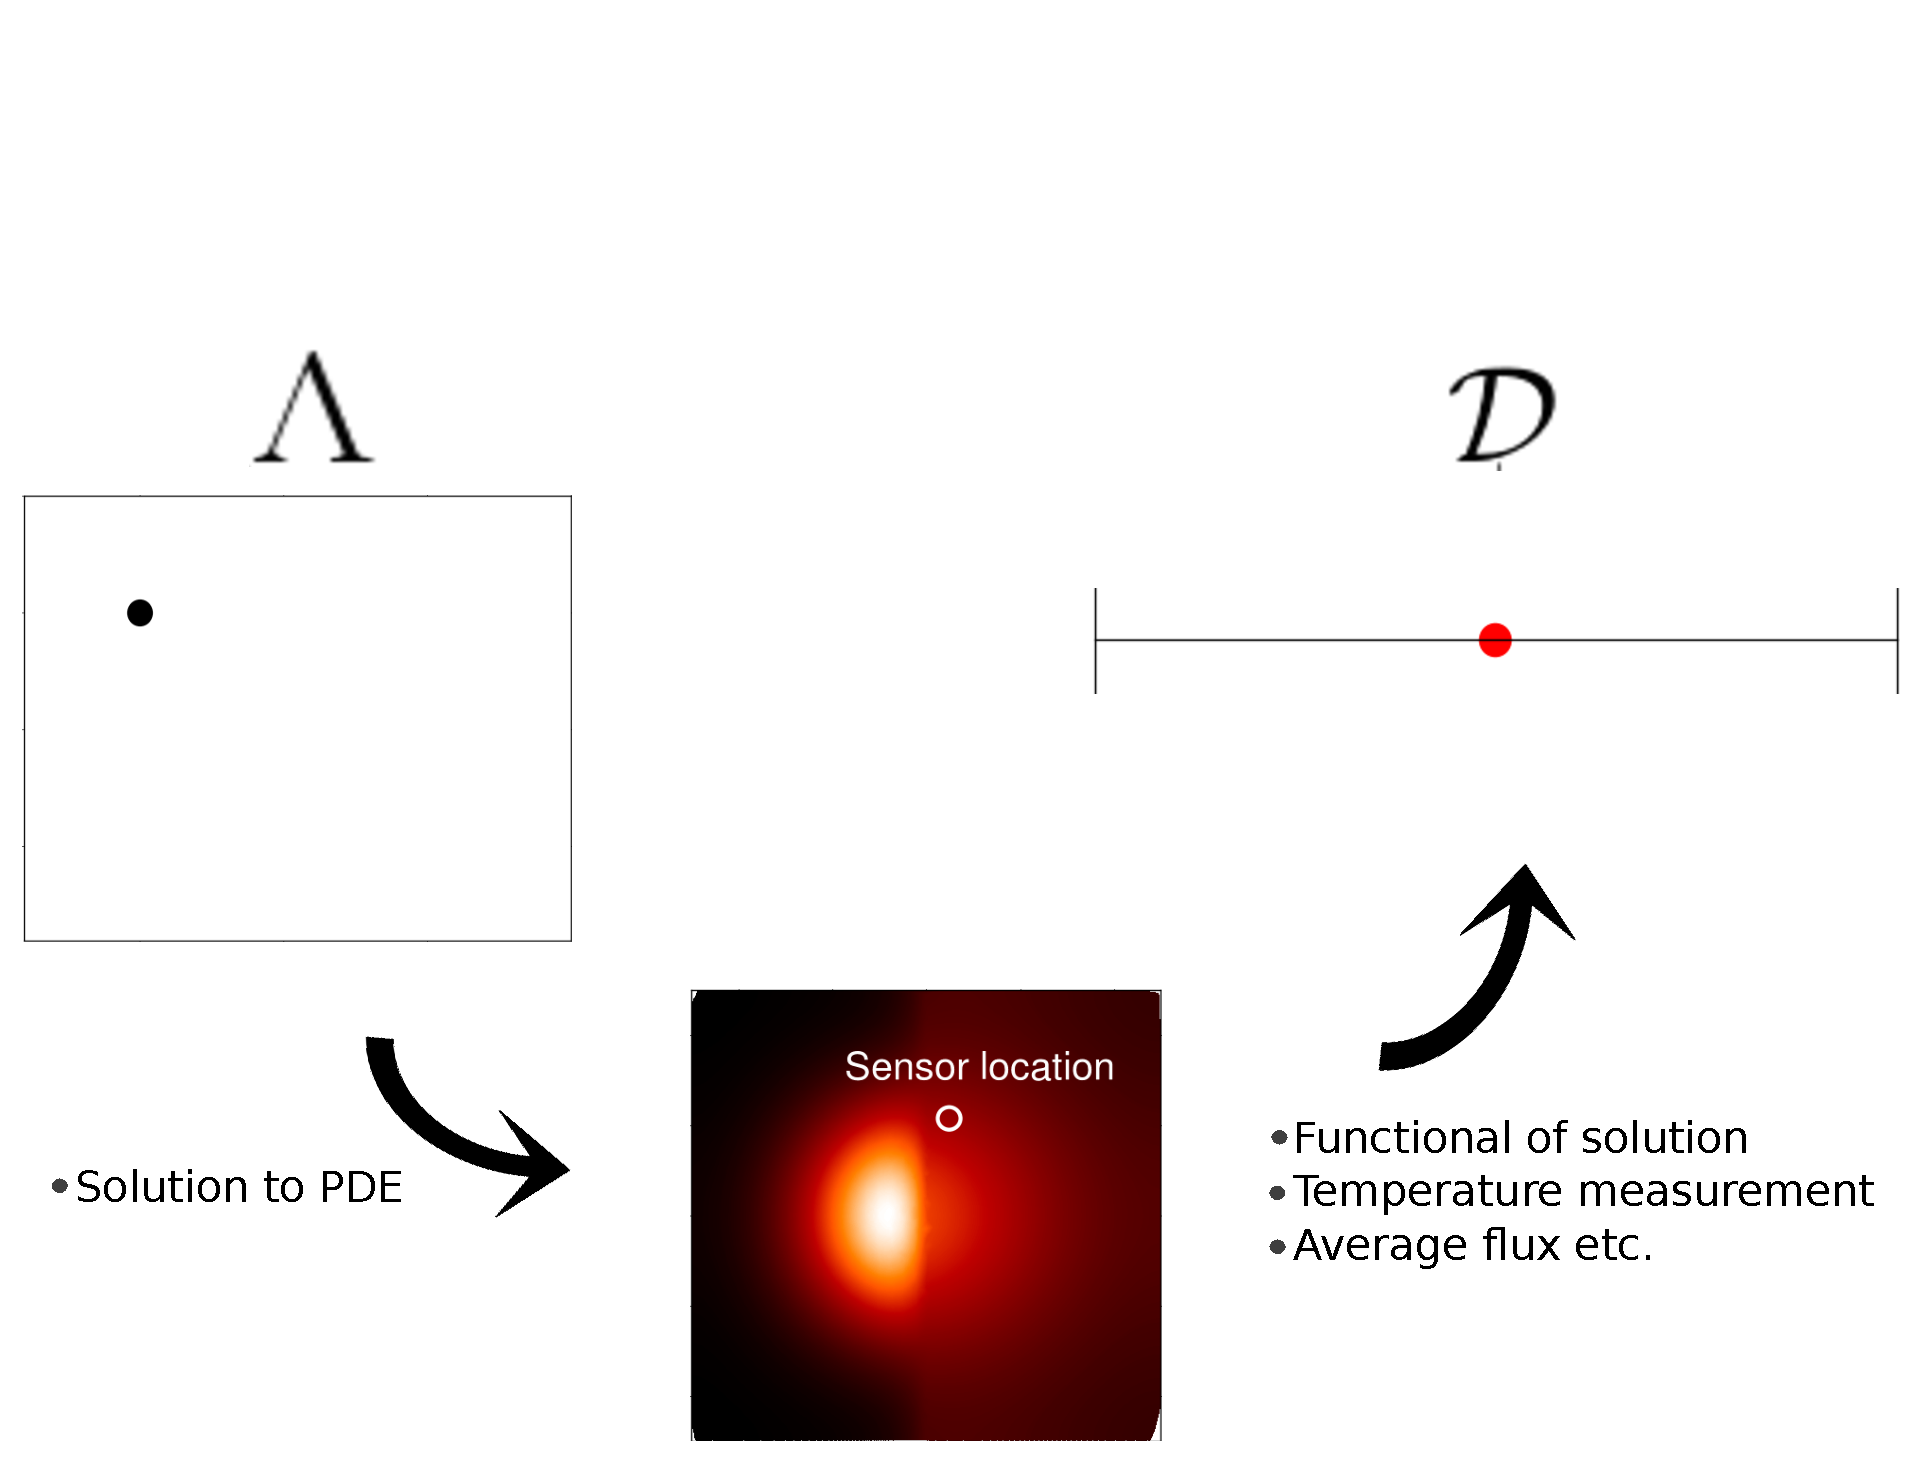
\includegraphics[width=0.85\textwidth]{./figures/threelevels/schematic_lambda_solution_data.pdf}
\end{figure}

}

\only<2>{

\begin{figure}[h]
	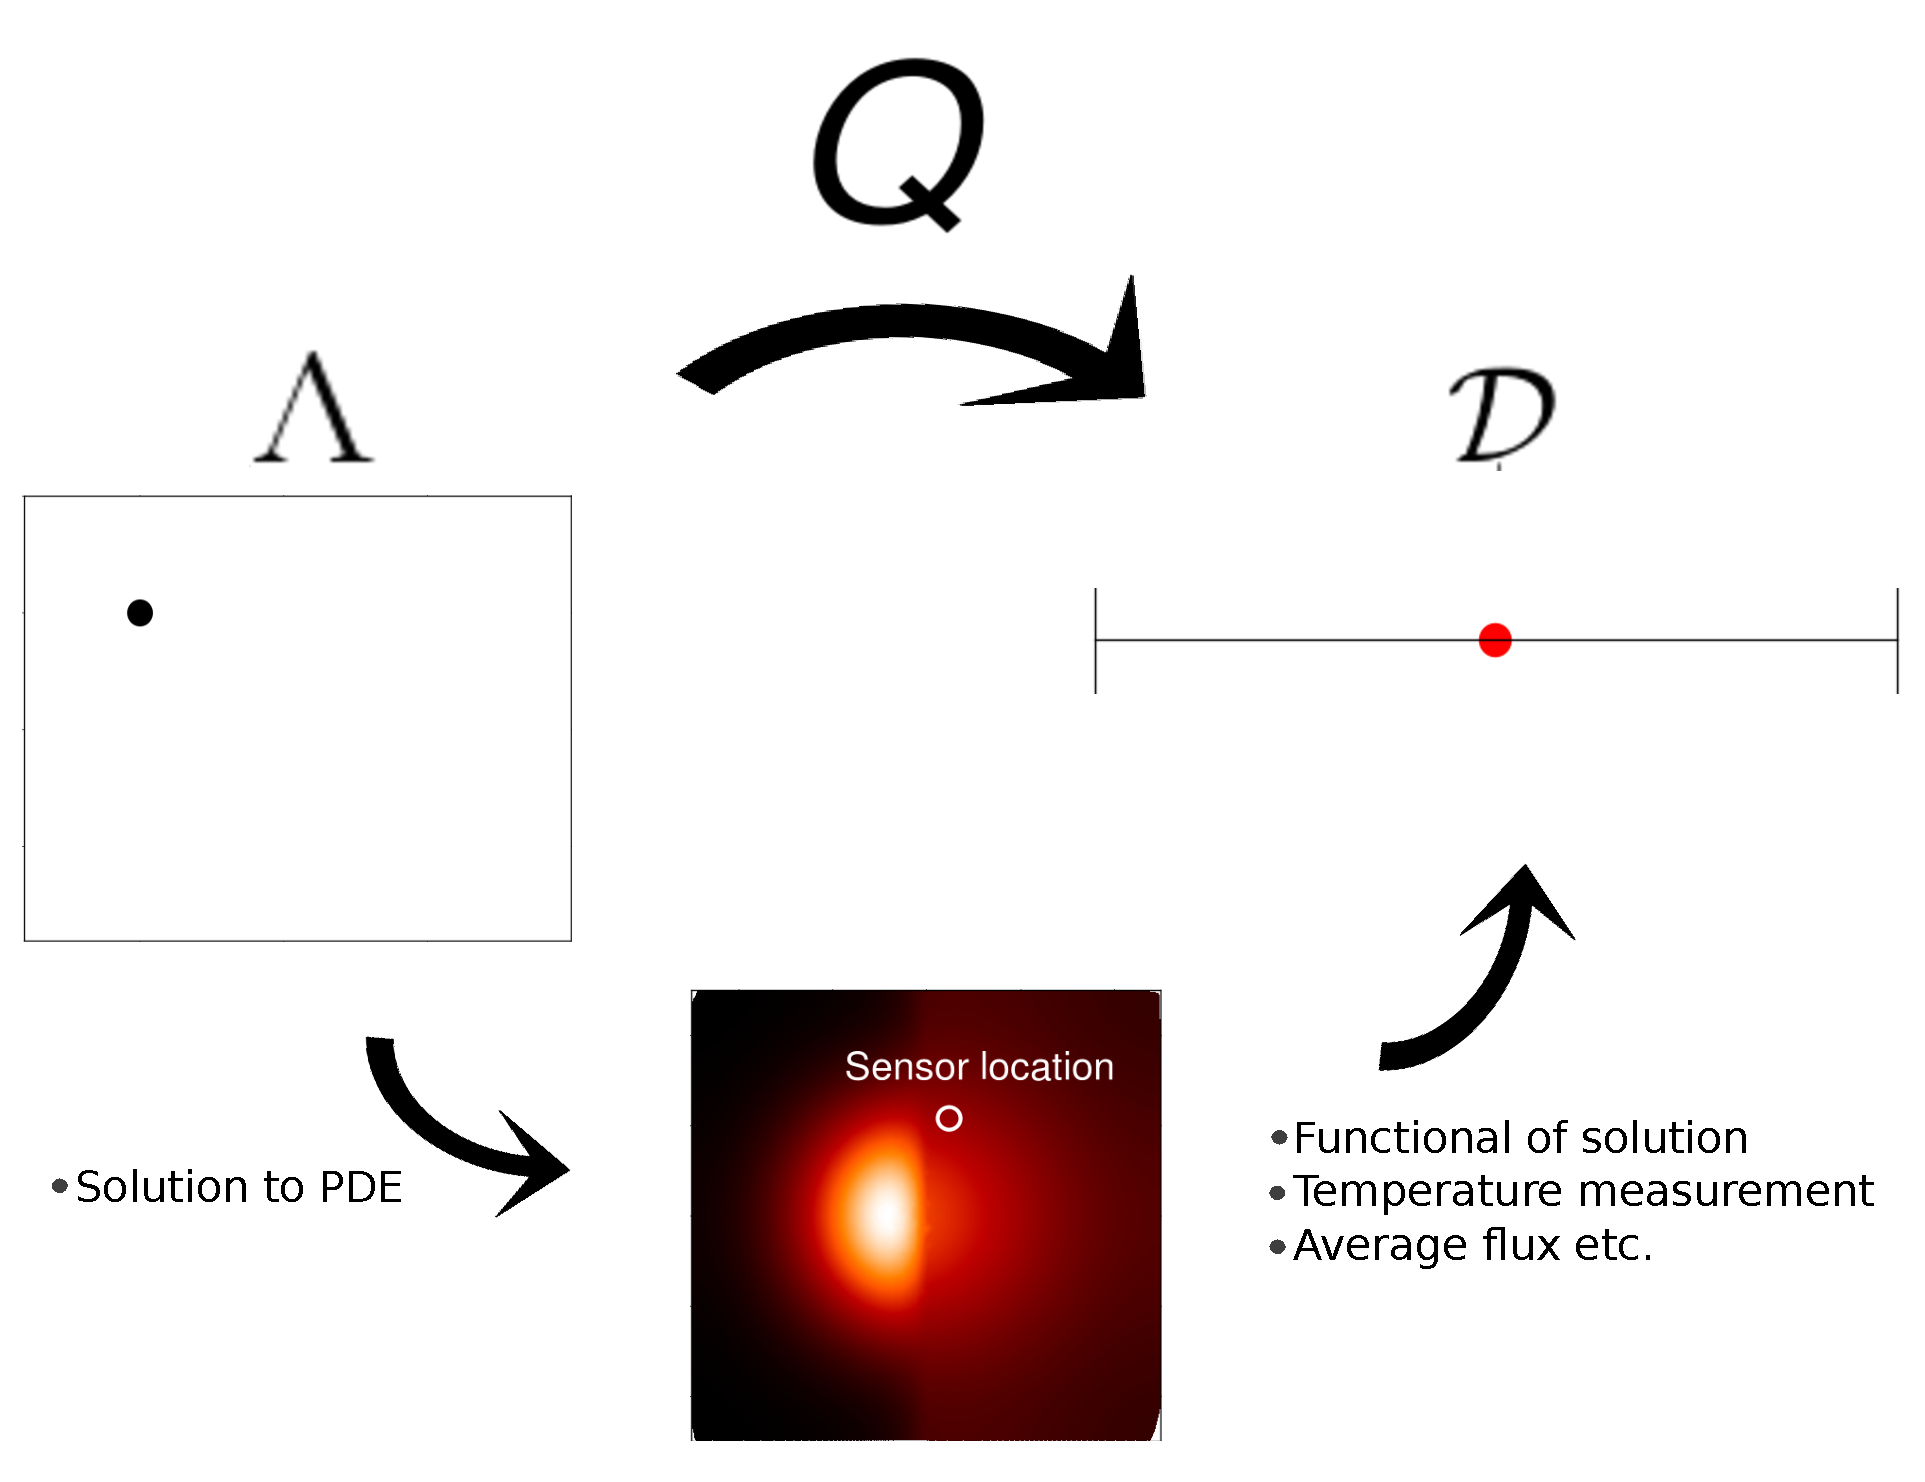
\includegraphics[width=0.85\textwidth]{./figures/threelevels/schematic_lambda_data.pdf}
\end{figure}

}

\only<3>{

\begin{figure}[h]
	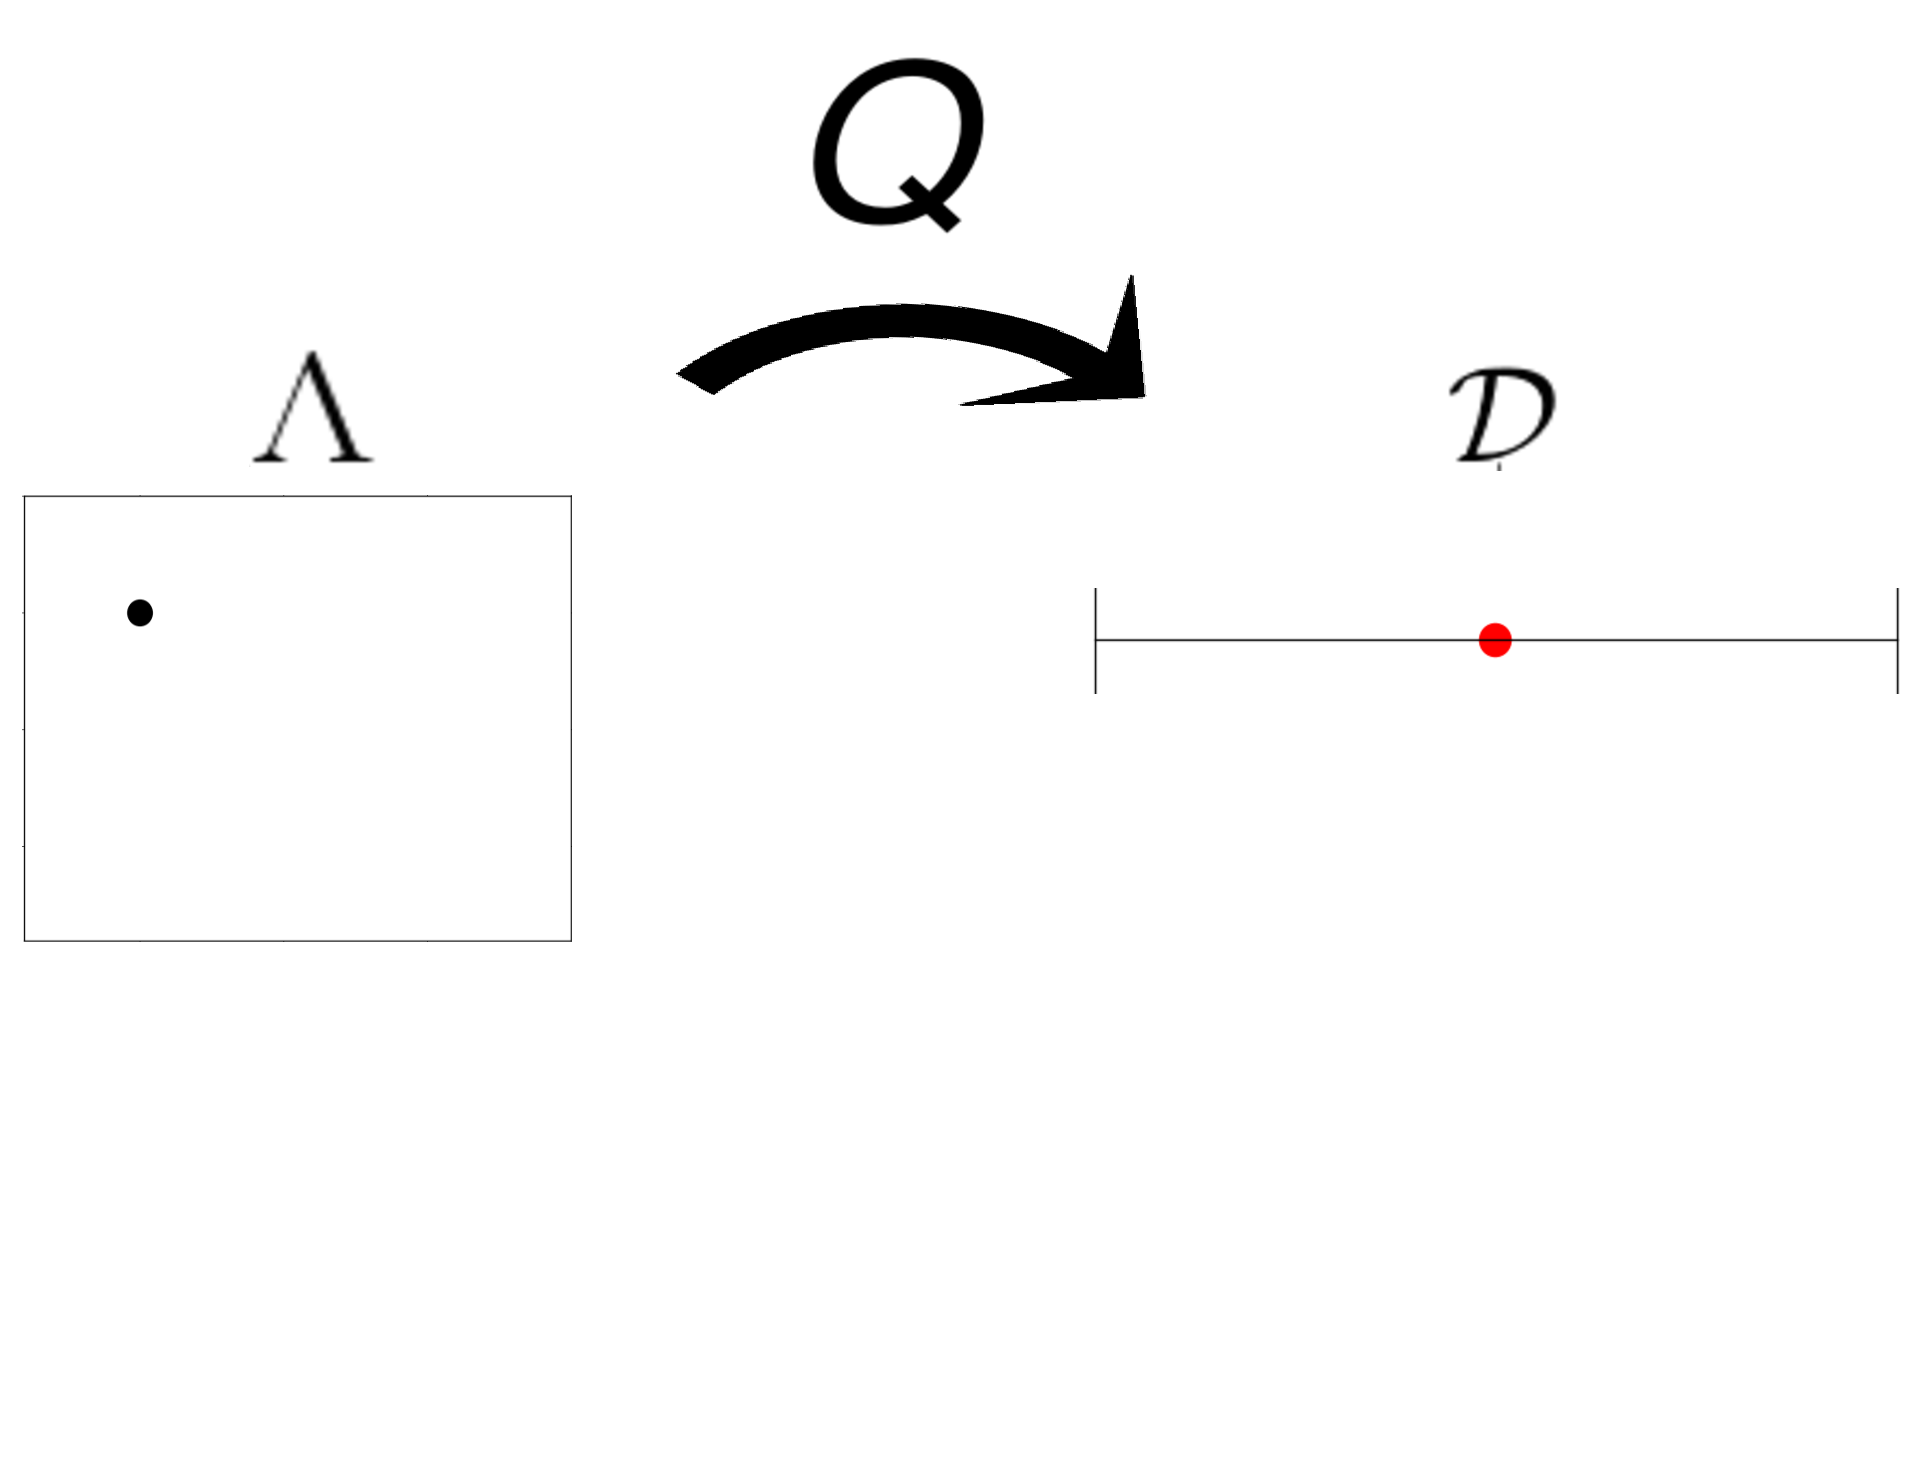
\includegraphics[width=0.85\textwidth]{./figures/threelevels/schematic_lambda_data_level1.pdf}
\end{figure}

}

\end{frame}

%%%%%%%%%%%%%%%%%%%%%%%%%%%%%%%%%%%%%%%%%%%%%%%%%%%%%%%%%%
\begin{frame}{A Forward UQ Problem}

\begin{figure}[h]
	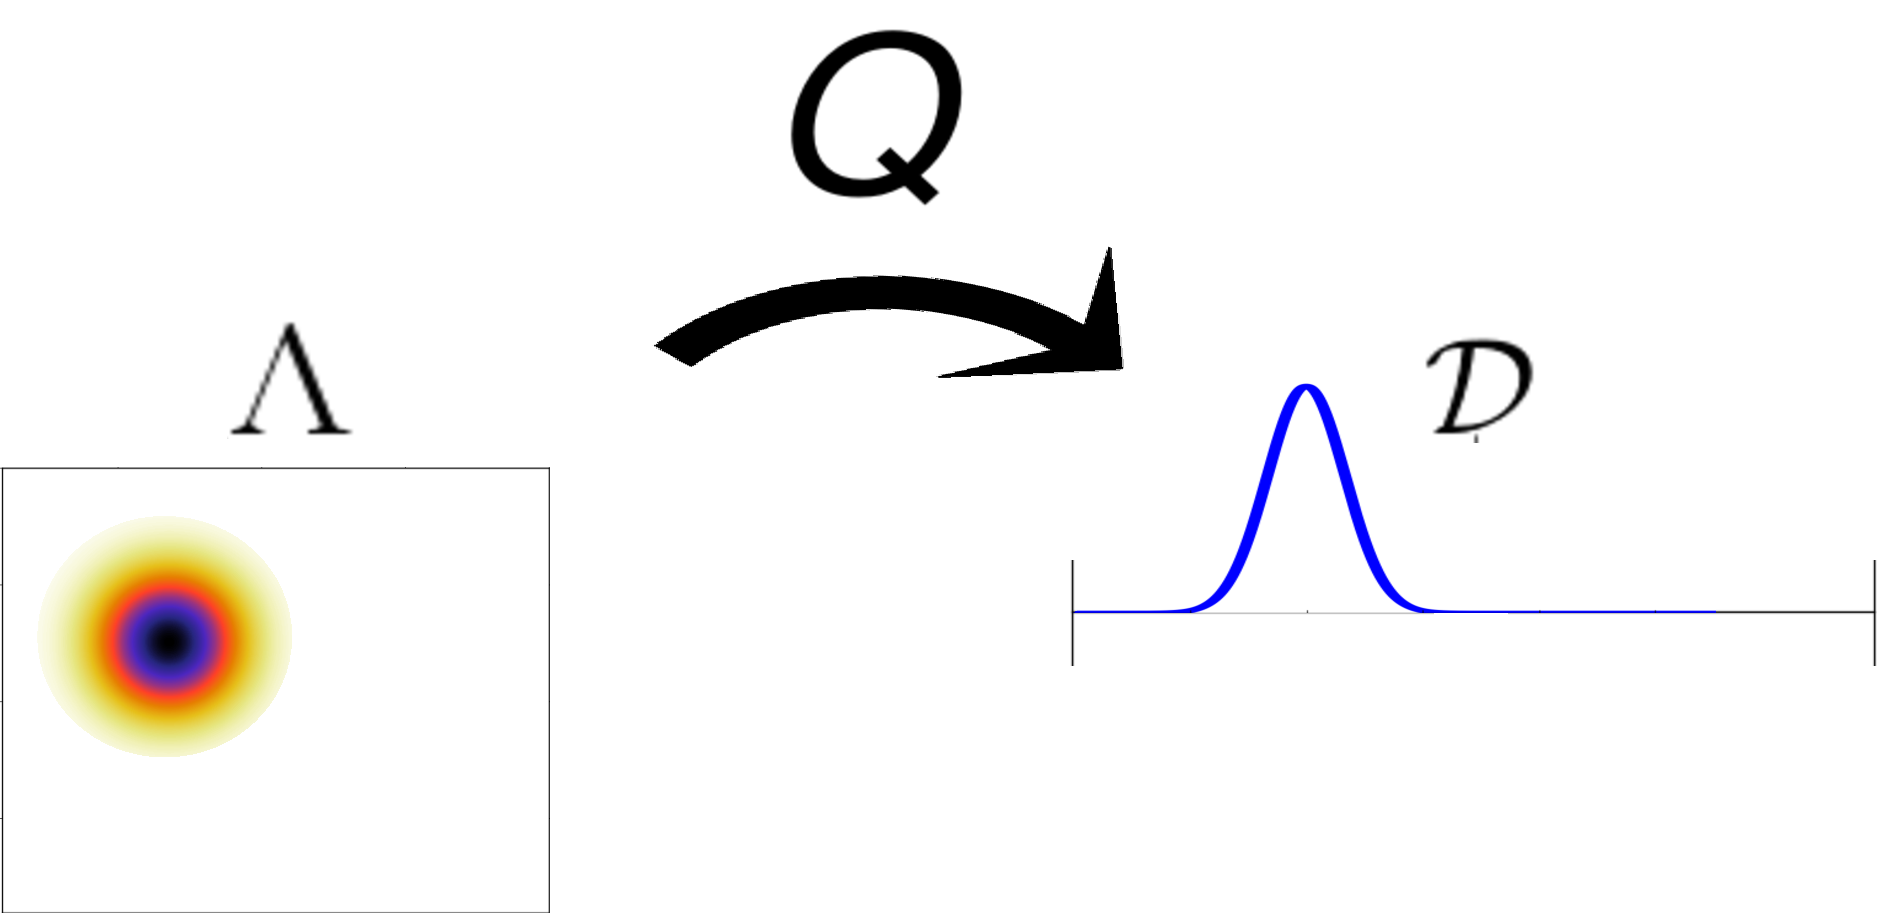
\includegraphics[width=0.85\textwidth]{./figures/threelevels/schematic_lambda_data_level3.pdf}
\end{figure}

{We denote the measurable spaces of parameters and data on the QoI as $(\pspace,\pborel)$ and $(\dspace,\dborel)$, respectively.}
\bigskip

\tdeepred{Given some prior density $\initial$ on $(\pspace,\pborel)$, we let $\predicted$ denote the push-forward of this density on $(\dspace,\dborel)$.}

\end{frame}

%%%%%%%%%%%%%%%%%%%%%%%%%%%%%%%%%%%%%%%%%%%%%%%%%%%%%%%%%%
\begin{frame}{The Inverse QoI Map}

\begin{figure}[h]
	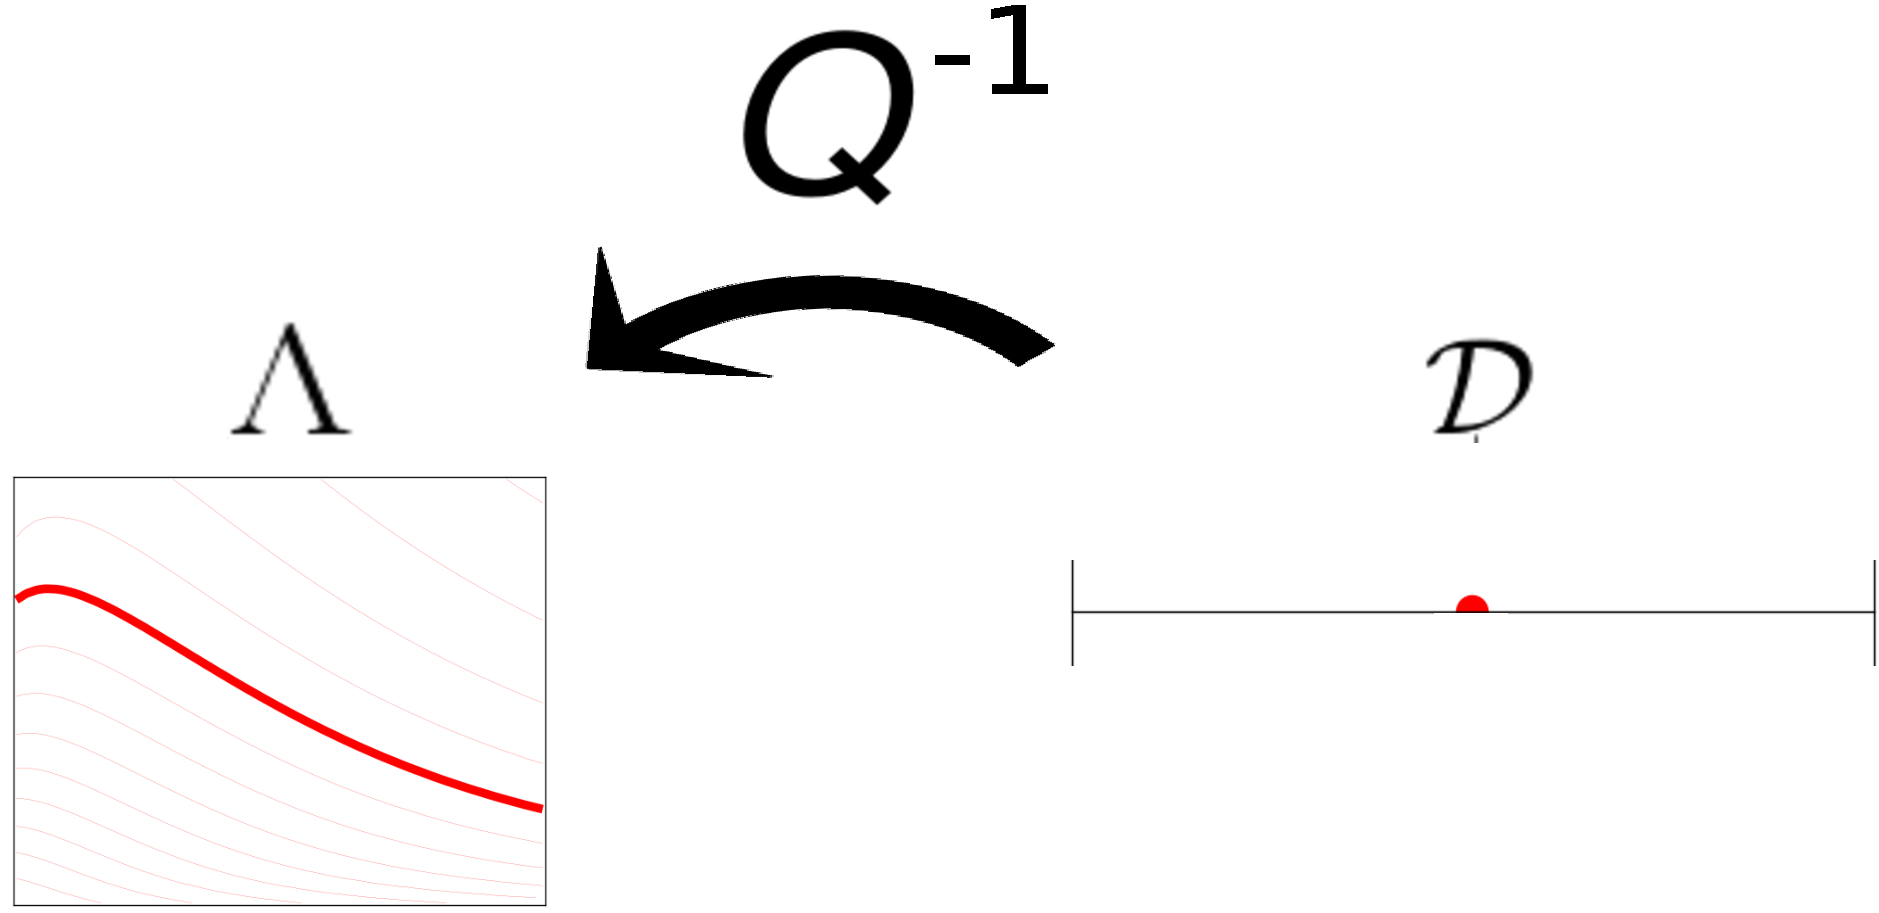
\includegraphics[width=0.85\textwidth]{./figures/threelevels/schematic_data_lambda_level1.pdf}
\end{figure}

\end{frame}

%%%%%%%%%%%%%%%%%%%%%%%%%%%%%%%%%%%%%%%%%%%%%%%%%%%%%%%%%%
\begin{frame}{An Inverse UQ Problem}

\begin{figure}[h]
	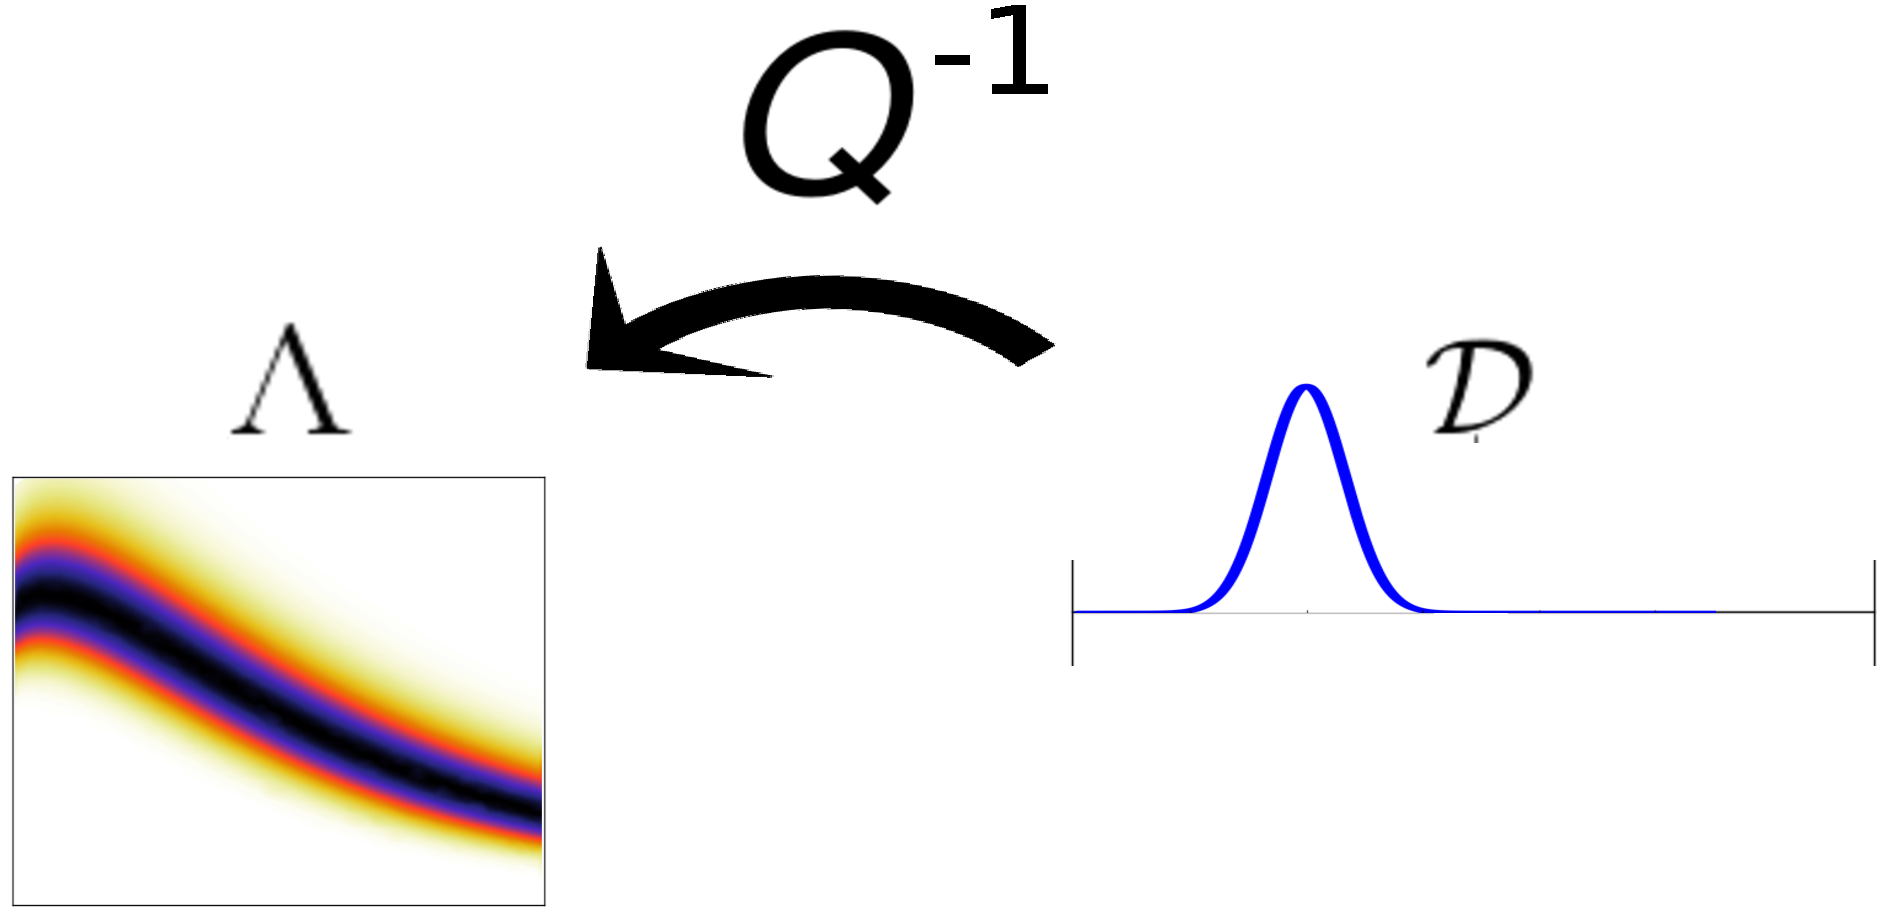
\includegraphics[width=0.85\textwidth]{./figures/threelevels/schematic_data_lambda_level3.pdf}
\end{figure}

\tdeepred{Given $\obs$ on $(\dspace,\dborel)$, we let $\predicted$ denote the pullback (consistent) density on $(\pspace,\pborel)$.}

\end{frame}



\subsection{The Stochastic Inverse Problem}
%%%%%%%%%%%%%%%%%%%%%%%%%%%%%%%%%%%%%%%%%%%%%%%%%%%%%%%%%%
\begin{frame}[t]

\begin{figure}
\centering
	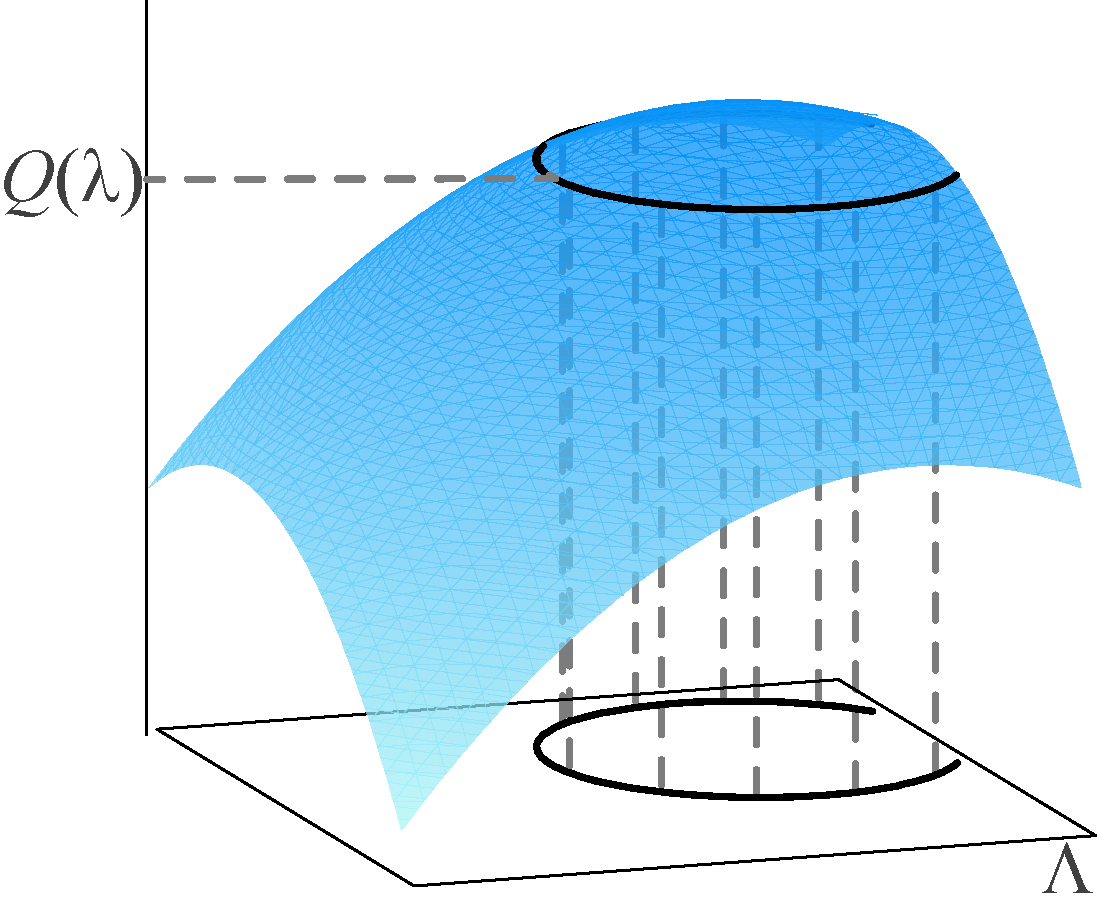
\includegraphics[width=.65\textwidth]{images/illustration1.pdf}<1>
	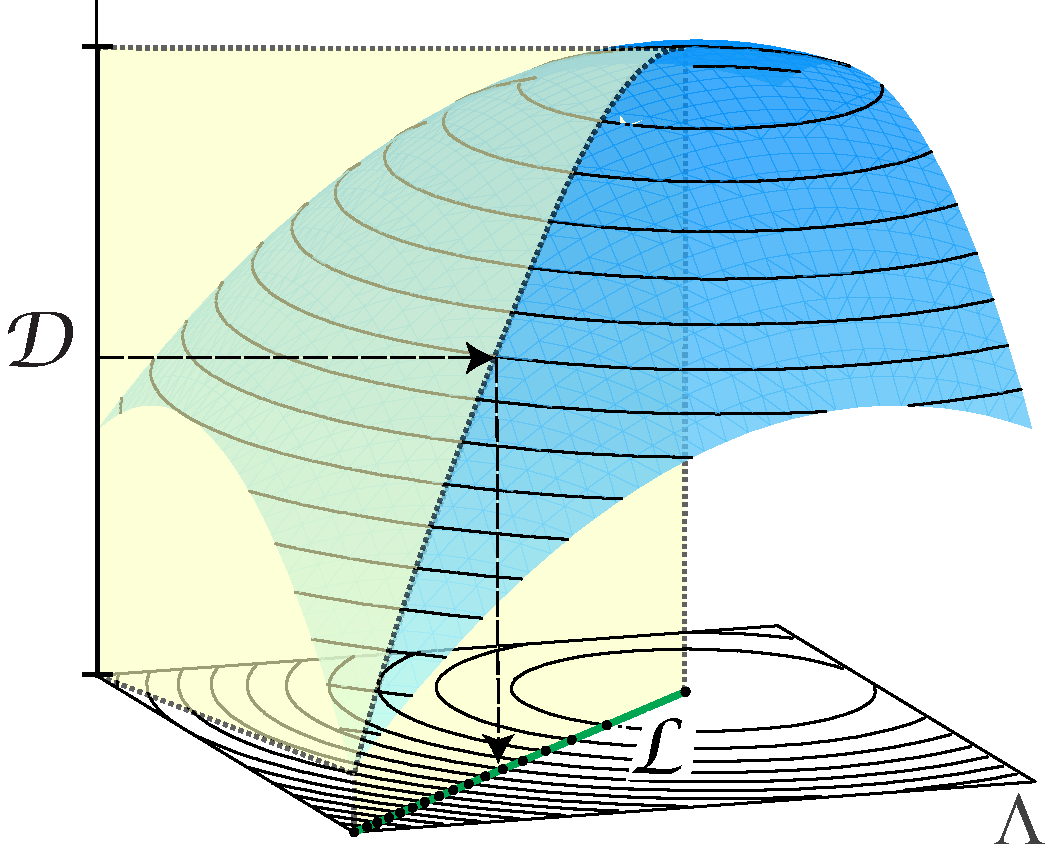
\includegraphics[width=.65\textwidth]{images/illustration2.pdf}<2>
	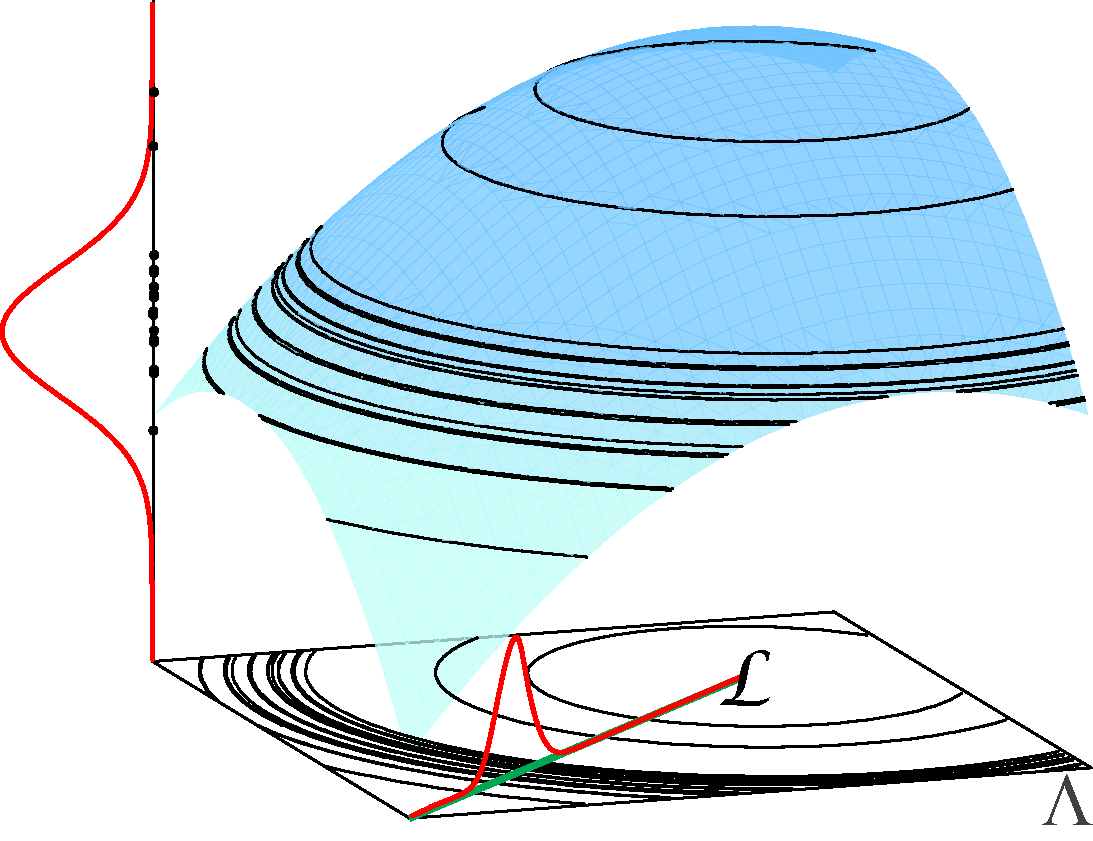
\includegraphics[width=.7\textwidth]{images/illustration3.pdf}<3>
\end{figure}
\begin{center}
{\scriptsize Figure adopted from \cite{BET14+} and used with permission}
\end{center}
\end{frame}

%%%%%%%%%%%%%%%%%%%%%%%%%%%%%%%%%%%%%%%%%%%%%%%%%%%%%%%%%%
\begin{frame}[t]

\begin{figure}
\centering
	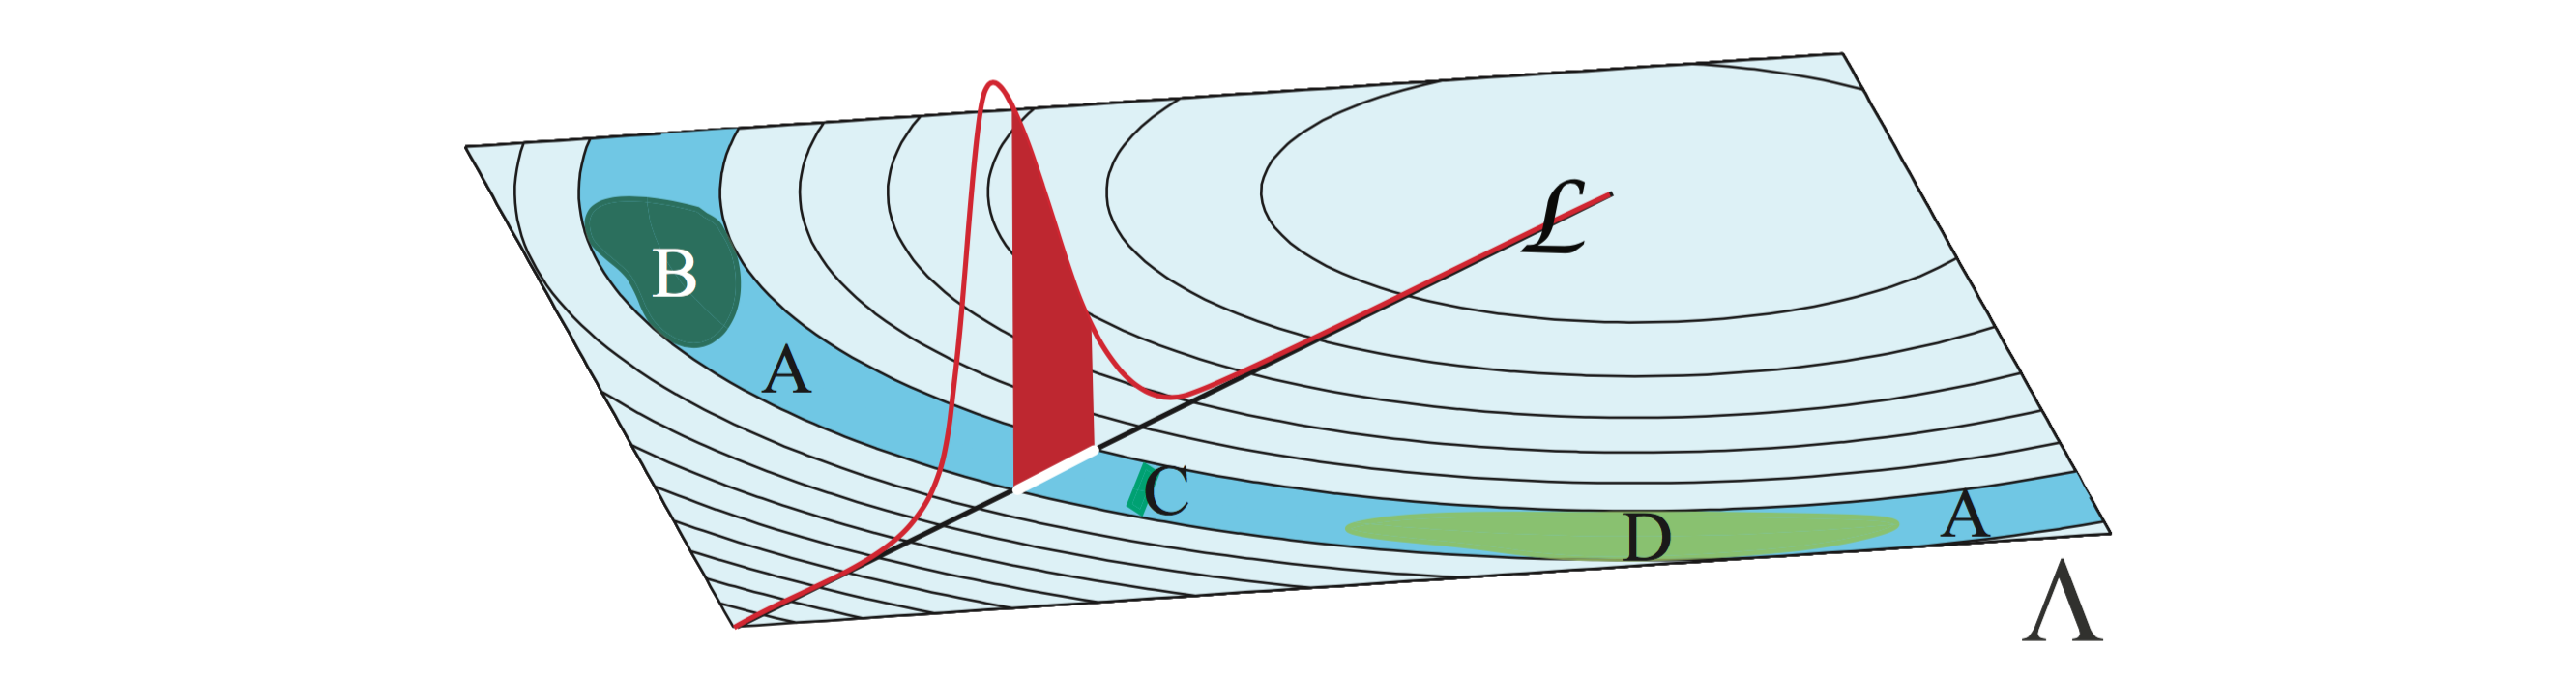
\includegraphics[width=1\textwidth]{images/troy_mt3contour.png}
\end{figure}
\begin{center}

{\scriptsize Figure adopted from \cite{BET14+} and used with permission}

\tdeepred{Key Question:} Distinguish (assign probability to) events that belong to same contour.
\end{center}
\end{frame}

\subsection{Problem Formulation and Solution}
%%%%%%%%%%%%%%%%%%%%%%%%%%%%%%%%%%%%%%%%%%%%%%%%%%%%%%%%%%%
\begin{frame}

\begin{defn}[Stochastic Forward Problem (SFP)]\label{defn:forward-problem}
  Given a probability measure $\PP_\pspace$ on $(\pspace, \pborel)$, and QoI map $\qoi$, the \emph{stochastic forward problem} is to determine a measure, $\PP_\dspace$, on $(\dspace, \dborel)$ that satisfies
  \begin{equation}\label{eq:forward-problem}
    \PP_\dspace (E) = \PP_\pspace \left ( \qoi^{-1}(E) \right ), \; \forall \; E \in \dborel.
  \end{equation}
\end{defn}

\end{frame}

\begin{frame}

\begin{defn}[Stochastic Forward Problem (SFP)]\label{defn:forward-problem}
  Given a probability measure $\PP_\pspace$ on $(\pspace, \pborel)$, and QoI map $\qoi$, the \emph{stochastic forward problem} is to determine a measure, $\PP_\dspace$, on $(\dspace, \dborel)$ that satisfies
  \begin{equation}\label{eq:forward-problem}
    \PP_\dspace (E) = \PP_\pspace \left ( \qoi^{-1}(E) \right ), \; \forall \; E \in \dborel.
  \end{equation}
\end{defn}

\begin{defn}[Stochastic Inverse Problem (SIP)]\label{defn:inverse-problem}
Given a probability measure, $\PP_\dspace$, on $(\dspace, \dborel)$ the \emph{stochastic inverse problem} is to determine a probability measure, $\PP_\pspace$, on $(\pspace, \pborel)$ satisfying
\begin{equation}\label{eq:inverse-problem}
\PP_\pspace (\qoi^{-1}(E)) = \PP_\dspace(E), \; \forall \; E \in \mathcal{B}_\dspace.
\end{equation}
\end{defn}

Equation~\eqref{eq:inverse-problem} is referred to as the \emph{consistency condition}.

\end{frame}


%%%%%%%%%%%%%%%%%%%%%%%%%%%%%%%%%%%%%%%%%%%%%%%%%%%%%%%%%%%
\begin{frame}

\begin{defn}[Consistent Solution and Density]\label{defn:consistent-solution}
  If $\PP_\pspace$ or $\PP_\dspace$ absolutely continuous w.r.t $\pmeas$ or $\dmeas$, resp, then we write

  \begin{equation*}
    \pp_\pspace := \frac{d\PP_\pspace}{d\pmeas} \;\text{ or }\; \pp_\dspace := \frac{d\PP_\dspace}{d\dmeas}
  \end{equation*}
  to denote the Radon-Nikodym derivatives of $\PP_\pspace$ and $\PP_\dspace$, resp.
  \bigskip

  In such a case, we can rewrite \eqref{eq:forward-problem} and \eqref{eq:inverse-problem} using these pdfs:
  \begin{equation*}
  \PP_\pspace (\qoi^{-1}(E)) = \int_{\qoi^{-1}(E)} \pp_\pspace \lam \, d\pmeas = \int_E \pp_\dspace \Q \, d\dmeas = \PP_\dspace(E)
  \end{equation*}

\end{defn}

\end{frame}


%%%%%%%%%%%%%%%%%%%%%%%%%%%%%%%%%%%%%%%%%%%%%%%%%%%%%%%%%%%
\begin{frame}

\begin{defn}[Initial Distribution]\label{defn:initial}
  When $\PP_\pspace$ in \eqref{eq:forward-problem} quantifies the characterization of uncertainty in parameter variability before observations on QoI are taken into account, it is referred to as the \emph{initial measure} $\initialP$.

  If a dominating measure $\mu_\pspace$ exists on $(\pspace, \pborel)$, the \emph{initial distribution} $\initial$ is given by the Radon-Nikodym derivative of $\initialP$ w.r.t the measure $\pmeas$.
\end{defn}

\end{frame}


%%%%%%%%%%%%%%%%%%%%%%%%%%%%%%%%%%%%%%%%%%%%%%%%%%%%%%%%%%%
\begin{frame}
\begin{defn}[Predicted Distribution]\label{defn:predicted}
 The \emph{predicted distribution} (or density) is the push-forward density of $\initial$ under the map $\qoi$, and is denoted as $\predicted$.

  Given as the Radon-Nikodym derivative (w.r.t $\dmeas$) of the pushforward measure
 \begin{equation}\label{eq:predicted}
    \predictedP (E) = \initialP \left ( \qoi^{-1}(E) \right ), \; \forall \; E \in \dborel.
  \end{equation}
\end{defn}


\end{frame}


%%%%%%%%%%%%%%%%%%%%%%%%%%%%%%%%%%%%%%%%%%%%%%%%%%%%%%%%%%%
\begin{frame}

\begin{defn}[Observed Distribution]\label{defn:observed}
When $\PP_\dspace$ in \eqref{eq:inverse-problem} quantifies the characterization of uncertainty in the QoI data, it is referred to as the \emph{observed measure}, $\observedP$.
\bigskip

Given a dominating $\mu_\dspace$ on $(\dspace, \dborel)$, the Radon-Nikodym derivative $\observedP$ w.r.t. $\dmeas$ is referred to as the  \emph{observed density} $\observed$.
\end{defn}

\end{frame}


%%%%%%%%%%%%%%%%%%%%%%%%%%%%%%%%%%%%%%%%%%%%%%%%%%%%%%%%%%
\begin{frame}{\it The one where we define the solution to the SIP.}

We now have all of the definitions required to summarize the density-based solution to the SIP, known as the \emph{updated density} as:
\vskip 10pt
\begin{equation}\label{eq:updated-pdf}
	\updated(\param) := \initial(\param)\frac{\observed(Q(\param))}{\predicted(Q(\param))}.
\end{equation}

\end{frame}

%
%
% %%%%%%%%%%%%%%%%%%%%%%%%%%%%%%%%%%%%%%%%%%%%%%%%%%%%%%%%%%
% \begin{frame}{Summarizing}
% \begin{itemize}
% 	\item ``Push-forward'' \textbf{initial} beliefs using $\qoi$ to \textbf{compare} to \textbf{observed} (data)
% 	\item Solve forward problem to construct solution to inverse problem
% 	\item The push-forward density of $\initial$ under the map $\qoi$ is denoted by $\predicted$
%
% 	\begin{defn}[Predicted Density]\label{defn:predicted}
% 		$\predicted$ is given as the Radon-Nikodym derivative (with respect to $\mu_\dspace$) of the push-forward probability measure defined by:
% 		\begin{equation}\label{eq:pred}
% 			\predictedP (E)  = \initialP \left ( \qoi^{-1}(E) \right ), \; \forall \; E \in \dborel.
% 		\end{equation}
% 	\end{defn}
%
% \end{itemize}
%
% \end{frame}
%
% %%%%%%%%%%%%%%%%%%%%%%%%%%%%%%%%%%%%%%%%%%%%%%%%%%%%%%%%%%
% \begin{frame}{The Updated Density solves the SIP}
% These definitions are combined to form the \textbf{updated density}:
% \begin{equation}\label{eq:up}
% \updated \lam = \initial \lam \frac{\observed \qlam }{\predicted \qlam }, \; \param, \in \pspace.
% \end{equation}
%
% \begin{itemize}
% 	\item $\observed$ and $\predicted$ defined on $(\dspace, \dborel)$ are evaluated at $\qlam$
% 	\item The map $\qoi$ impacts the structure of the update
% 	\item $\dspace$ itself depends on $\qoi$
% 	\item Primary effort in solving for $\updated$ (in \eqref{eq:up}) requires constructing $\predicted$
% 	\item This is because $\initial$ and $\observed$ are given \emph{a priori} (often parametric)
% 	\item Updated derived through use of Disintegration Theorem in \cite{BJW18a}
% 	\item Existence and Uniqueness given a \emph{predictability assumption}
% \end{itemize}
% \end{frame}
%
%
%
% \subsection{Properties and Assumptions of the Update}
% %%%%%%%%%%%%%%%%%%%%%%%%%%%%%%%%%%%%%%%%%%%%%%%%%%%%%%%%%%
% \begin{frame}
% \begin{assumption}[Predictability Assumption]\label{as:pred}
% 	The measure associated with $\observed$ is absolutely continuous with respect to the measure associated with $\predicted$.
% \end{assumption}
%
%
% The requirement is guaranteed if the following is satisfied:
%
% \begin{equation}\label{eq:pred}
% 	\exists \; C>0 \text{ s.t. } \observed (d) \leq C \predicted (d) \text{ for a.e. } d\in \dspace,
% \end{equation}
%
% where $d = \qlam$ for some $\param \in \pspace$.
% By \cite{BJW18}, if \eqref{as:pred} holds, we have:
%
% \begin{theorem}[Existence and Uniqueness]
% 	For any set $A\in \pborel$, the solution $\updatedP$ given defined by
% 	\begin{equation}\label{eq:cb_sol}
% 		\updatedP (A) = \int_\dspace \left (  \int_{\pspace \in \qoi^{-1}(d)}  \initial\param \frac{\observed(d)}{\predicted(d)} \, d\mu_{\pspace, d} \param \right ) \, d\mu_\dspace(d), \; \forall \; A \in \pborel
% 	\end{equation}
%
% 	is a consistent solution, and is unique up to choice of $\initialP$ on $(\pspace, \pborel)$.
% \end{theorem}
%
% \end{frame}
%
%
% %%%%%%%%%%%%%%%%%%%%%%%%%%%%%%%%%%%%%%%%%%%%%%%%%%%%%%%%%%
% \begin{frame}{Stability}
%
% All the stability and convergence results presented are with respect to:
% \vspace{0.5in}
%
% \begin{defn}{Total Variation / Statistical Distance}
% 	\begin{equation}\label{eq:tv}
% 		d_{\text{TV}} (\PP_f, \PP_g) := \int \abs{f - g} \, d\mu,
% 	\end{equation}
% where $f,g$ are the densities (Radon-Nikodym derivatives with respect to $\mu$) associated with measures $\PP_f, \PP_g$, respectively.
% \end{defn}
%
% \end{frame}
%
% %%%%%%%%%%%%%%%%%%%%%%%%%%%%%%%%%%%%%%%%%%%%%%%%%%%%%%%%%%
% \begin{frame}
%
% \begin{defn}[Stability of Updates I]\label{defn:stableobs}
% 	We say that $\updatedP$ is \emph{stable} with respect to perturbations in $\observedP$ if for all $\eps > 0$, there exists a $\delta > 0$ such that
% 	\begin{equation}
% 		d_{\text{TV}} (\observedP, \widehat{\observedP}) < \delta \implies d_{\text{TV}} (\updatedP, \widehat{\updatedP}) < \eps.
% 	\end{equation}
% \end{defn}
%
% \vspace{0.5in}
% In \cite{BJW18}, it is shown that $d_{\text{TV}} (\widehat{\updatedP}, \updatedP) = d_{\text{TV}} (\widehat{\observedP}, \observedP)$, implying that:
% \vspace{0.5in}
%
% \begin{theorem}
% 	$\updatedP$ is stable with respect to perturbations in $\observedP$.
% \end{theorem}
%
% \end{frame}
%
% %%%%%%%%%%%%%%%%%%%%%%%%%%%%%%%%%%%%%%%%%%%%%%%%%%%%%%%%%%
% \begin{frame}
% \begin{defn}[Stability of Updates II]\label{defn:stableinitial}
% Let $\sett{\PP_{\pspace, d}}{d\in\dspace}{}$ and $\sett{\widehat{\PP_{\pspace, d}}}{d\in\dspace}{}$ be the conditional probabilities defined by the disintegration of $\initialP$ and $\widehat{\initialP}$, respectively.
%
% We say that $\updatedP$ is \emph{stable} with respect to perturbations in $\initialP$ if for all $\eps > 0$, there exists a $\delta > 0$ such that for almost every $d\in\supp(\observed)$,
% \begin{equation}\label{eq:stableinitial}
% d_{\text{TV}} (\PP_{\pspace, d}, \widehat{\PP_{\pspace, d}}) < \delta \implies d_{\text{TV}} (\updatedP, \widehat{\updatedP}) < \eps.
% \end{equation}
% \end{defn}
%
% \begin{theorem}
% $\updatedP$ is stable with respect to perturbations in the initial.
% \label{thm:stableinitial}
% \end{theorem}
%
%
% \end{frame}
%
% %%%%%%%%%%%%%%%%%%%%%%%%%%%%%%%%%%%%%%%%%%%%%%%%%%%%%%%%%%
% \begin{frame}{Properties of the Updated Density}
% \begin{itemize}
%
% 	\item Taken together, these stability results provide assurances that the updated we obtain is accurate up to the level of experimental error polluting $\observed$ and error in incorrectly specifying initial assumptions.
% 	\item Given that specifying the definition of a ``true'' initial is somewhat nebulous, we are less interested in the consequences of the latter conclusion.
% 	\item Generating samples from $\predicted$ requires a numerical approximation to $\predicted$, which introduces \textbf{additional errors} in $\predicted$.
%
% \end{itemize}
%
% \end{frame}
%
%
% \subsection{Numerical Approximation and Sampling}
% %%%%%%%%%%%%%%%%%%%%%%%%%%%%%%%%%%%%%%%%%%%%%%%%%%%%%%%%%%
% \begin{frame}
% \begin{itemize}
% 	\item Let $\widehat{\predicted}$ be a computational approximation to $\predicted$ and $\widehat{\updated}$ the associated approximate updated $\updated$
% 	\item The conditional densities from the Disintegration theorem are
% \[
% \frac{\widehat{d\PP_{\pspace, d}}}{d\mu_{\pspace, d}\lam} = \frac{\initial\lam}{ \widehat{\predicted (d)} }
% \]
% \vspace{0.25in}
% 	\item To approximate the push-forward of the initial density, we require:
% \begin{assumption}\label{as:predx}
% There exists some $C>0$ such that
% \[
% \observed (d) \leq C \widehat{\predicted(d)} \text{ for a.e. } d\in \dspace.
% \]
% \end{assumption}
%
% \end{itemize}
%
% \end{frame}
%
%
% %%%%%%%%%%%%%%%%%%%%%%%%%%%%%%%%%%%%%%%%%%%%%%%%%%%%%%%%%%
% \begin{frame}
% \begin{assumption}\label{as:predx}
% There exists some $C>0$ such that
% \[
% \observed (d) \leq C \widehat{\predicted(d)} \text{ for a.e. } d\in \dspace.
% \]
% \end{assumption}
%
% If this assumption is satisfied, we can prove the following cite{BJW18}:
%
% \begin{theorem}
% The error in the approximate updated is:
% \begin{equation}\label{eq:pred_bound}
% d_{\text{TV}} (\updatedP, \widehat{\updatedP}) \leq C d_{\text{TV}} (\predictedP, \widehat{\predictedP}),
% \end{equation}
% where the $C$ is the constant taken from \eqref{as:predx}.
% \end{theorem}
%
% \end{frame}


%%%%%%%%%%%%%%%%%%%%%%%%%%%%%%%%%%%%%%%%%%%%%%%%%%%%%%%%%%
\begin{frame}[t]{The one with some practical considerations.}

\begin{itemize}
	\item We approximate $\predicted$ using density estimation on forward propagation of samples from $\initial$
	\item May evaluate $\updated$ directly for any sample of $\pspace$ (one model solve)
	\item Accuracy of the computed updated density is proportional to accuracy of approximation of the predicted density
	\item We (currently) use Gaussian KDE
	\begin{itemize}
			\item Let $\dimD$ be the dimension of $\dspace$
			\item Let $\nsamps$ be the number of samples from $\initial$ propagated through $\qoi$
			\item Converges at a rate of $\mathcal{O}(\nsamps^{-4/(4+\dimD)})$ in mean-squared error
			\item Converges at a rate of $\mathcal{O}(\nsamps^{-2/(4+\dimD)})$ in $L^1$-error
	\end{itemize}
  \item Stable w.r.t. perturbations in the Total Variation metric
\end{itemize}
\end{frame}



%%%%%%%%%%%%%%%%%%%%%%%%%%%%%%%%%%%%%%%%%%%%%%%%%%%%%%%%%%%
%%%%%%%%%%%%%%%%%%%%%%%%%%%%%%%%%%%%%%%%%%%%%%%%%%%%%%%%%%%
\section{Notation and Terminology}
%%%%%%%%%%%%%%%%%%%%%%%%%%%%%%%%%%%%%%%%%%%%%%%%%%%%%%%%%%%
%%%%%%%%%%%%%%%%%%%%%%%%%%%%%%%%%%%%%%%%%%%%%%%%%%%%%%%%%%%


%%%%%%%%%%%%%%%%%%%%%%%%%%%%%%%%%%%%%%%%%%%%%%%%%%%%%%%%%%%
\subsection{Measure Theory 101}
%%%%%%%%%%%%%%%%%%%%%%%%%%%%%%%%%%%%%%%%%%%%%%%%%%%%%%%%%%%

\begin{frame}[t]
%\vskip 25pt
\centering
\begin{figure}
\centering

The one with the background on inverse problems.

\end{figure}

\end{frame}


%%%%%%%%%%%%%%%%%%%%%%%%%%%%%%%%%%%%%%%%%%%%%%%%%%%%%%%%%%%
\subsection{A Philosophical Distinction}
%%%%%%%%%%%%%%%%%%%%%%%%%%%%%%%%%%%%%%%%%%%%%%%%%%%%%%%%%%%

\begin{frame}[t]
%\vskip 25pt
\centering
\begin{figure}
\centering

The one where we distinguish ourselves from the Bayesians.

\end{figure}

\end{frame}


%%%%%%%%%%%%%%%%%%%%%%%%%%%%%%%%%%%%%%%%%%%%%%%%%%%%%%%%%%%
%%%%%%%%%%%%%%%%%%%%%%%%%%%%%%%%%%%%%%%%%%%%%%%%%%%%%%%%%%%
\section{Parameter Identification and the MUD Point}
%%%%%%%%%%%%%%%%%%%%%%%%%%%%%%%%%%%%%%%%%%%%%%%%%%%%%%%%%%%
%%%%%%%%%%%%%%%%%%%%%%%%%%%%%%%%%%%%%%%%%%%%%%%%%%%%%%%%%%%

%%%%%%%%%%%%%%%%%%%%%%%%%%%%%%%%%%%%%%%%%%%%%%%%%%%%%%%%%%%
\begin{frame}{\it The one where we define the Maximal Updated Density (MUD) point.}

\begin{equation}\label{eq:mudpt_inital_defn}
	\mudpt := \argmax {\updated}(\param)
\end{equation}

\end{frame}

\begin{frame}[t]{\it The one where we create a unifying framework.}

\begin{itemize}
  \item Recall $\norm{\mathbf{x}}_C^2 := (\mathbf{x}, \mathbf{x})_C = \mathbf{x}^T C \mathbf{x}$. \\

  \bigskip
  \item Non-degenerative $\predictedCov^{-1}$, $\observedCov^{-1}$, $\initialCov^{-1}$ play the role of $C$. \\

  \bigskip
  \bigskip
  \item Suppose that $\initial = \prior \sim \mathcal{N}(\param_0, \initialCov)$.

  \bigskip
  \item Suppose $\qoi$ is linear and that $\observed = \pi_\text{like} \sim \mathcal{N}(\observedMean, \observedCov)$.

  \bigskip
  \bigskip
  \item Linearity of $\qoi$ implies that $Q(\param)=A\param$ for some $A\in\RR^{d\times p}$, and that $\predicted \sim \mathcal{N}(Q(\param_0), \predictedCov)$, where

  \begin{equation}\label{eq:predictCov}
  	\predictedCov := A\initialCov A^\top.
  \end{equation}

\end{itemize}


\end{frame}

%%%%%%%%%%%%%%%%%%%%%%%%%%%%%%%%%%%%%%%%%%%%%%%%%%%%%%%%%%
\subsection{Theory of Regularization}
%%%%%%%%%%%%%%%%%%%%%%%%%%%%%%%%%%%%%%%%%%%%%%%%%%%%%%%%%%

\begin{frame}{\it The one with the regularization equations.}

\begin{table}[htbp]
\centering
\begin{equation*}
\begin{split}
\posterior(\param\,|\,d) &= \frac{\prior(\param)\pi_\text{like}(d\,|\,\param)}{\int_{\pspace} \pi_\text{like}(d\, |\, \param)  \prior(\param) d\pmeas} \\
& \\
\updated(\param) &= \initial(\param) \frac{\observed(Q(\param))}{\predicted(Q(\param))}
\end{split}
\end{equation*}

\bigskip
\begin{tabular}{|c|c|}
\hline
& \\
  Tikhonov & $T(\param):=\norm{Q(\param)-\observedMean}_{\observedCov^{-1}}^2 +
      \norm{\param-\initialMean}_{\initialCov^{-1}}^2$ \\
& \\
\hline & \\
  Data-Consistent & $J(\param):=T(\param) - \norm{Q(\param)-Q(\initialMean)}_{\predictedCov^{-1}}^2$ \\
& \\
  \hline
\end{tabular}
% \caption{The $\param$ which minimizes these functionals also maximizes the updated PDF (left) and the Bayesian posterior PDF (right).
%
% $T(\param)$ is the typical functional often associated with Tikhonov regularization.
%
% The $J(\param)$ has an additional term subtracted from $T(\param)$ coming from the predicted density that serves as ``unregularization'' in data--informed directions.}
  \label{tab:func_comparisons}
\end{table}


\end{frame}



%%%%%%%%%%%%%%%%%%%%%%%%%%%%%%%%%%%%%%%%%%%%%%%%%%%%%%%%%%%
\subsection{Linear Example}
%%%%%%%%%%%%%%%%%%%%%%%%%%%%%%%%%%%%%%%%%%%%%%%%%%%%%%%%%%%

%%%%%%%%%%%%%%%%%%%%%%%%%%%%%%%%%%%%%%%%%%%%%%%%%%%%%%%%%%%
\begin{frame}{\it The one where an example highlights a key difference.}

\begin{itemize}
\item $A=\mat{cc}{1 & 1}$

\bigskip
\item 2-D input, 1-D output $\implies$ rank-deficient

\bigskip
\item Details:

\begin{equation*}
\begin{split}
	\initialMean = \mat{cc}{0.25 & 0.25}^\top \\ \\
  \initialCov = \mat{cc}{1 & -0.25 \\ -0.25 & 0.5} \\ \\
  \observedMean=1, \text{ and } \observedCov = \mat{c}{0.25}
\end{split}
\end{equation*}

\end{itemize}
\end{frame}

%%%%%%%%%%%%%%%%%%%%%%%%%%%%%%%%%%%%%%%%%%%%%%%%%%%%%%%%%%%
\begin{frame}{\it The one that kind of says it all.}
%\vskip 25pt
\centering
\begin{figure}
\centering

\begin{figure}
   % 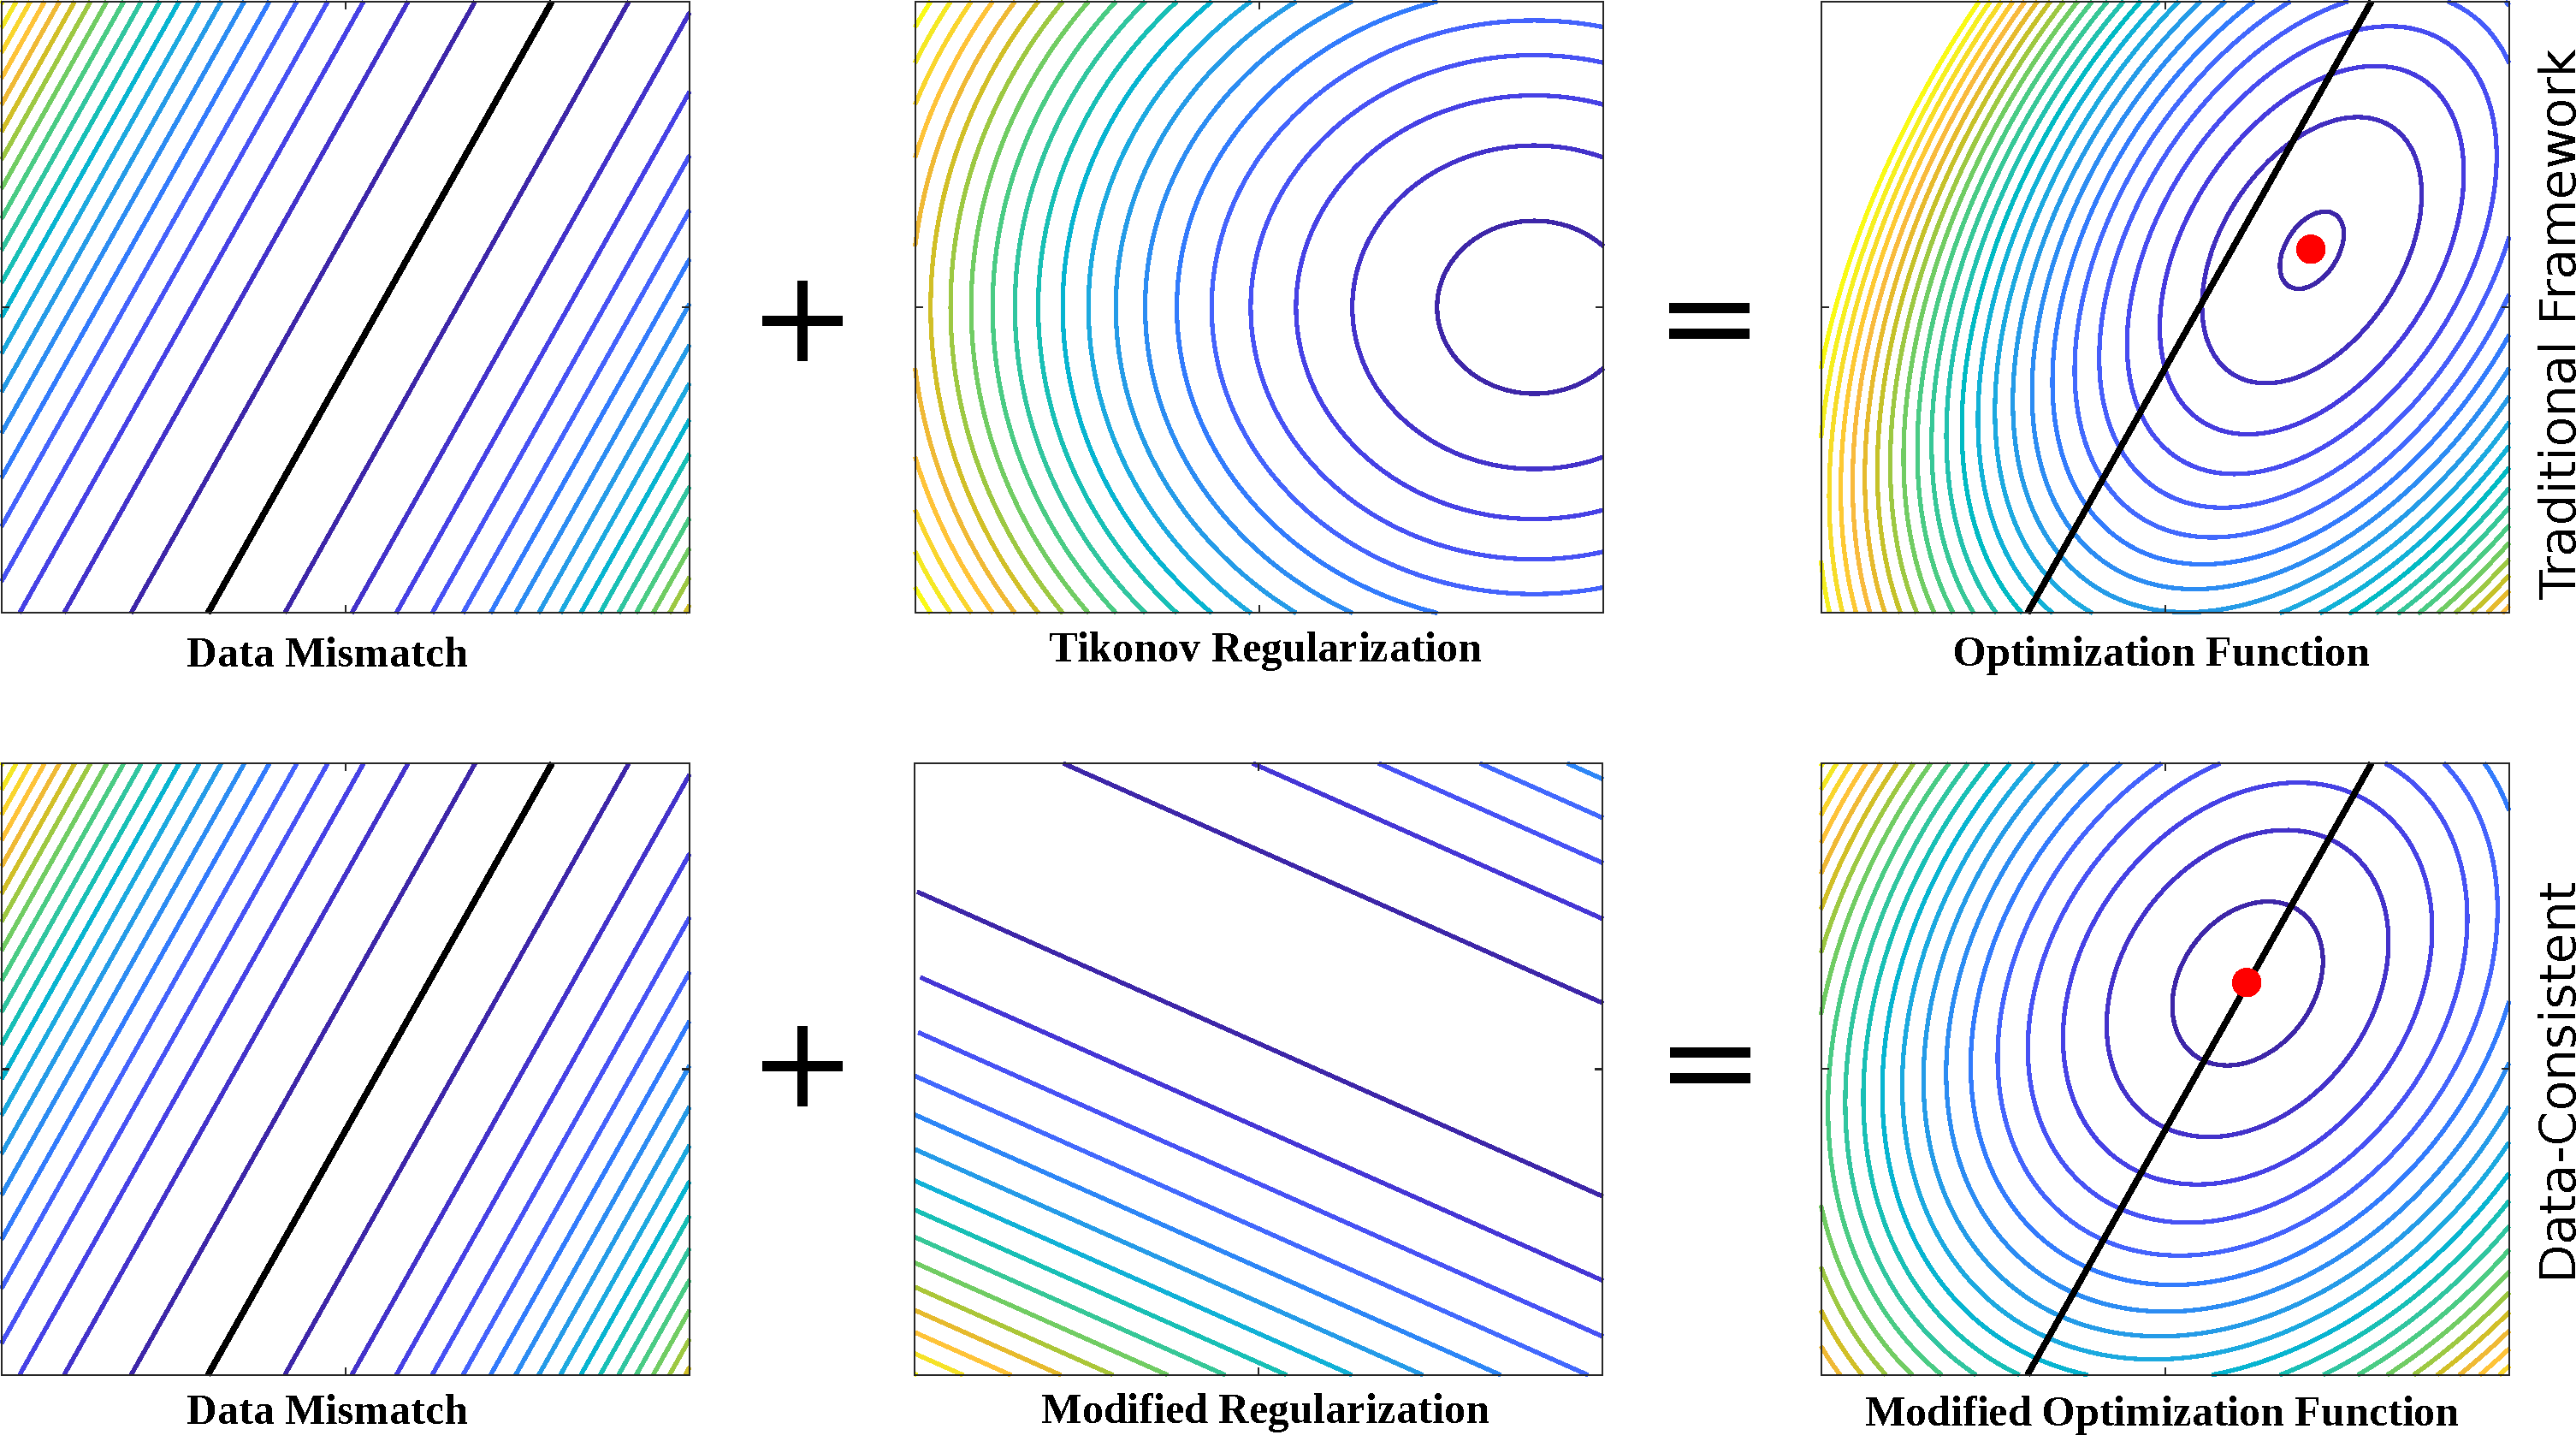
\includegraphics[width=\linewidth]{figures/Regularization-all-in-one.pdf}
  \centering
  \begin{tabular}{|ccc|}
    \hline
      \subf{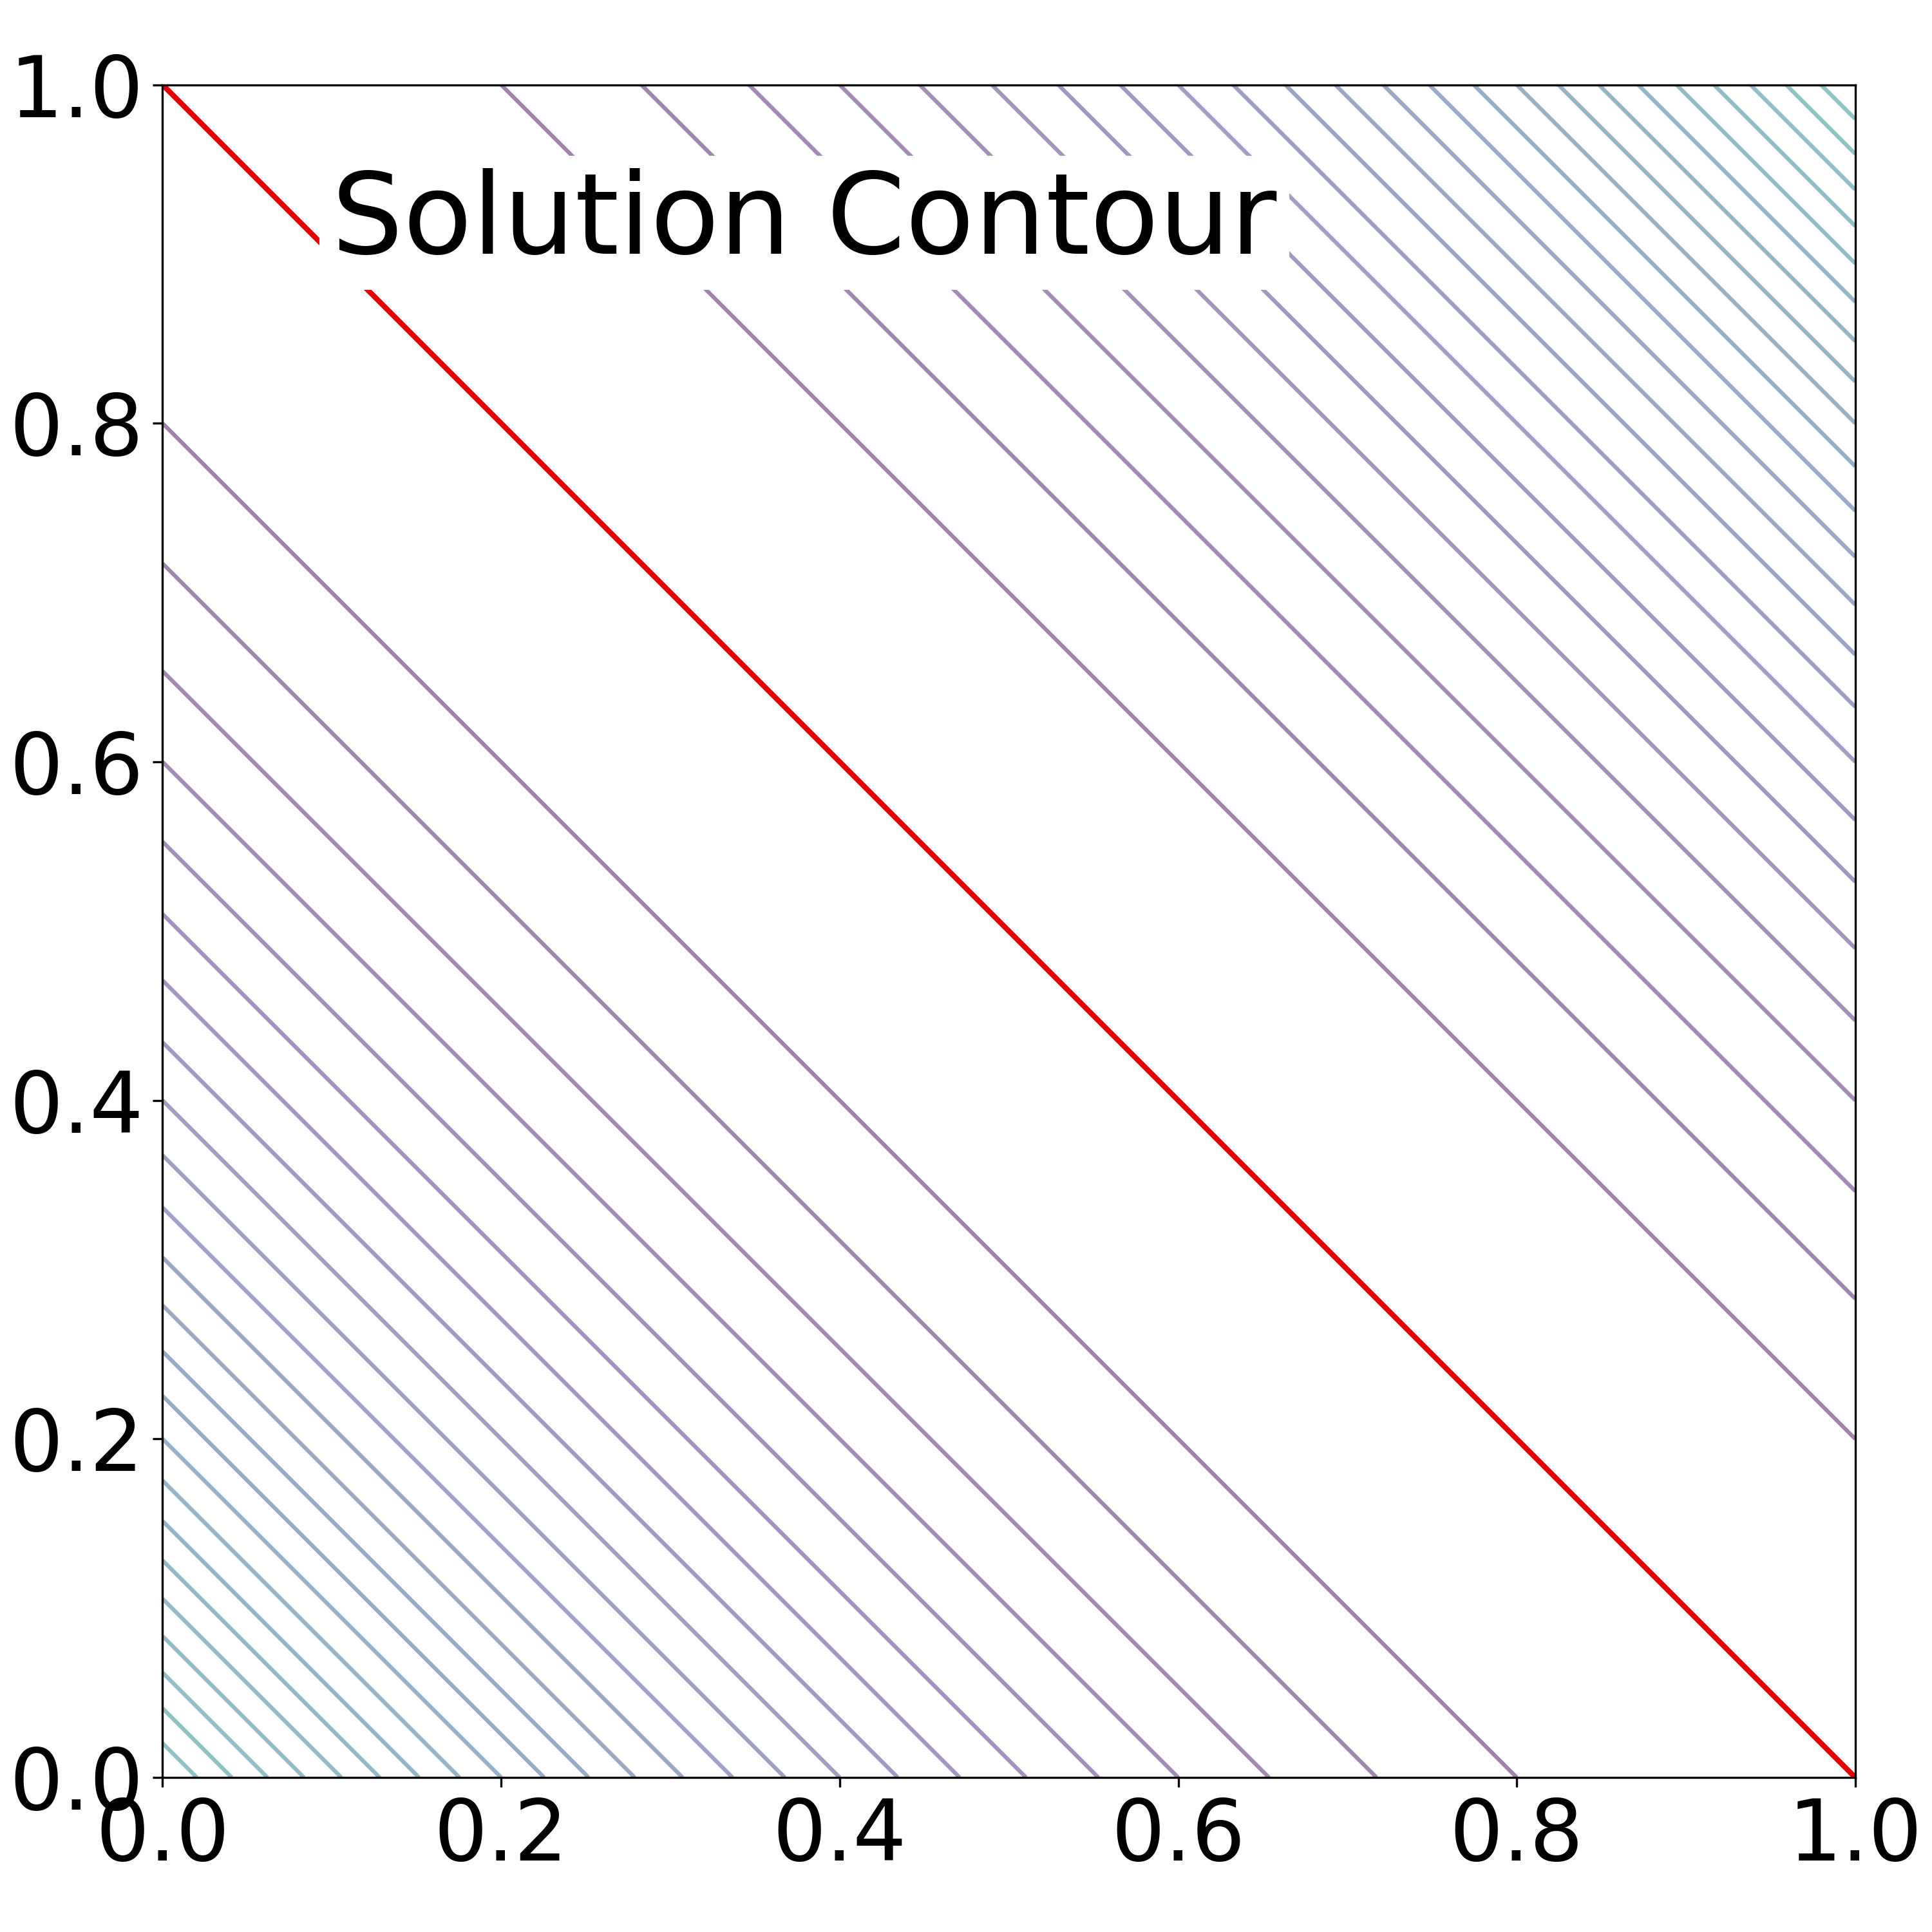
\includegraphics[width=0.25\linewidth]{figures/data_mismatch_contour.png}}
      {data mismatch}
    &
      \subf{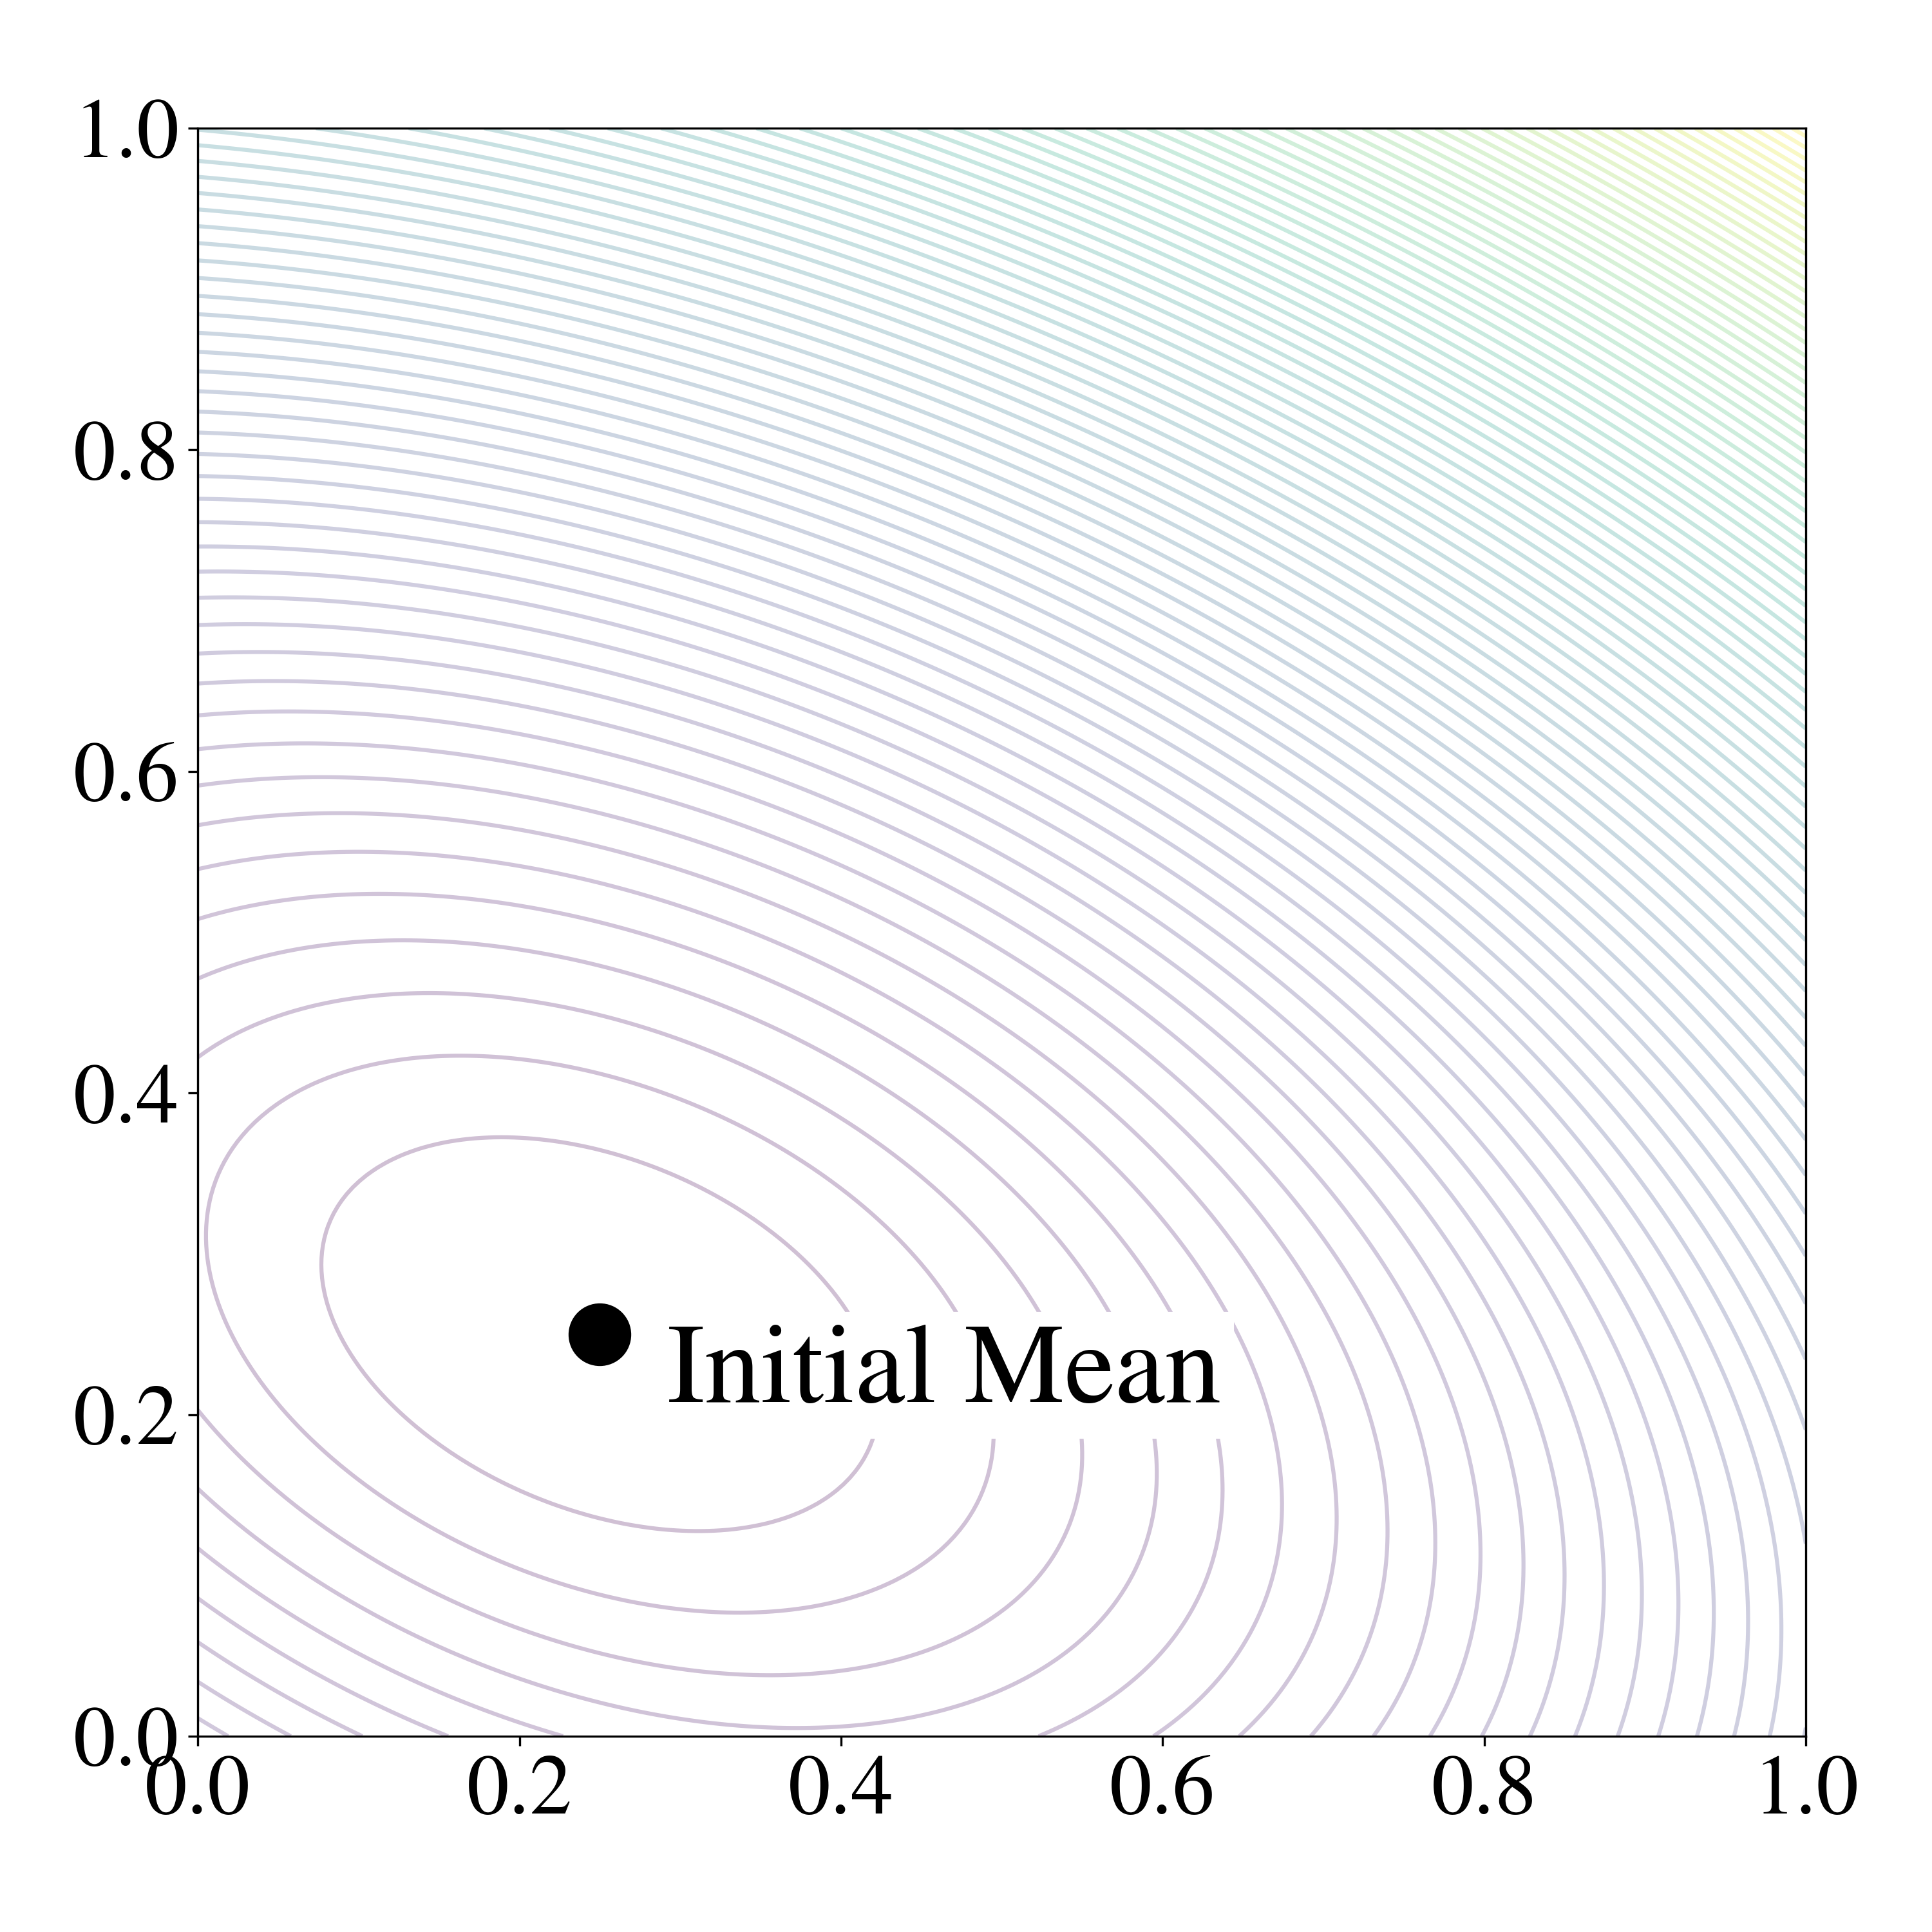
\includegraphics[width=0.25\linewidth]{figures/tikonov_contour.png}}
      {regularization}
    &
      \subf{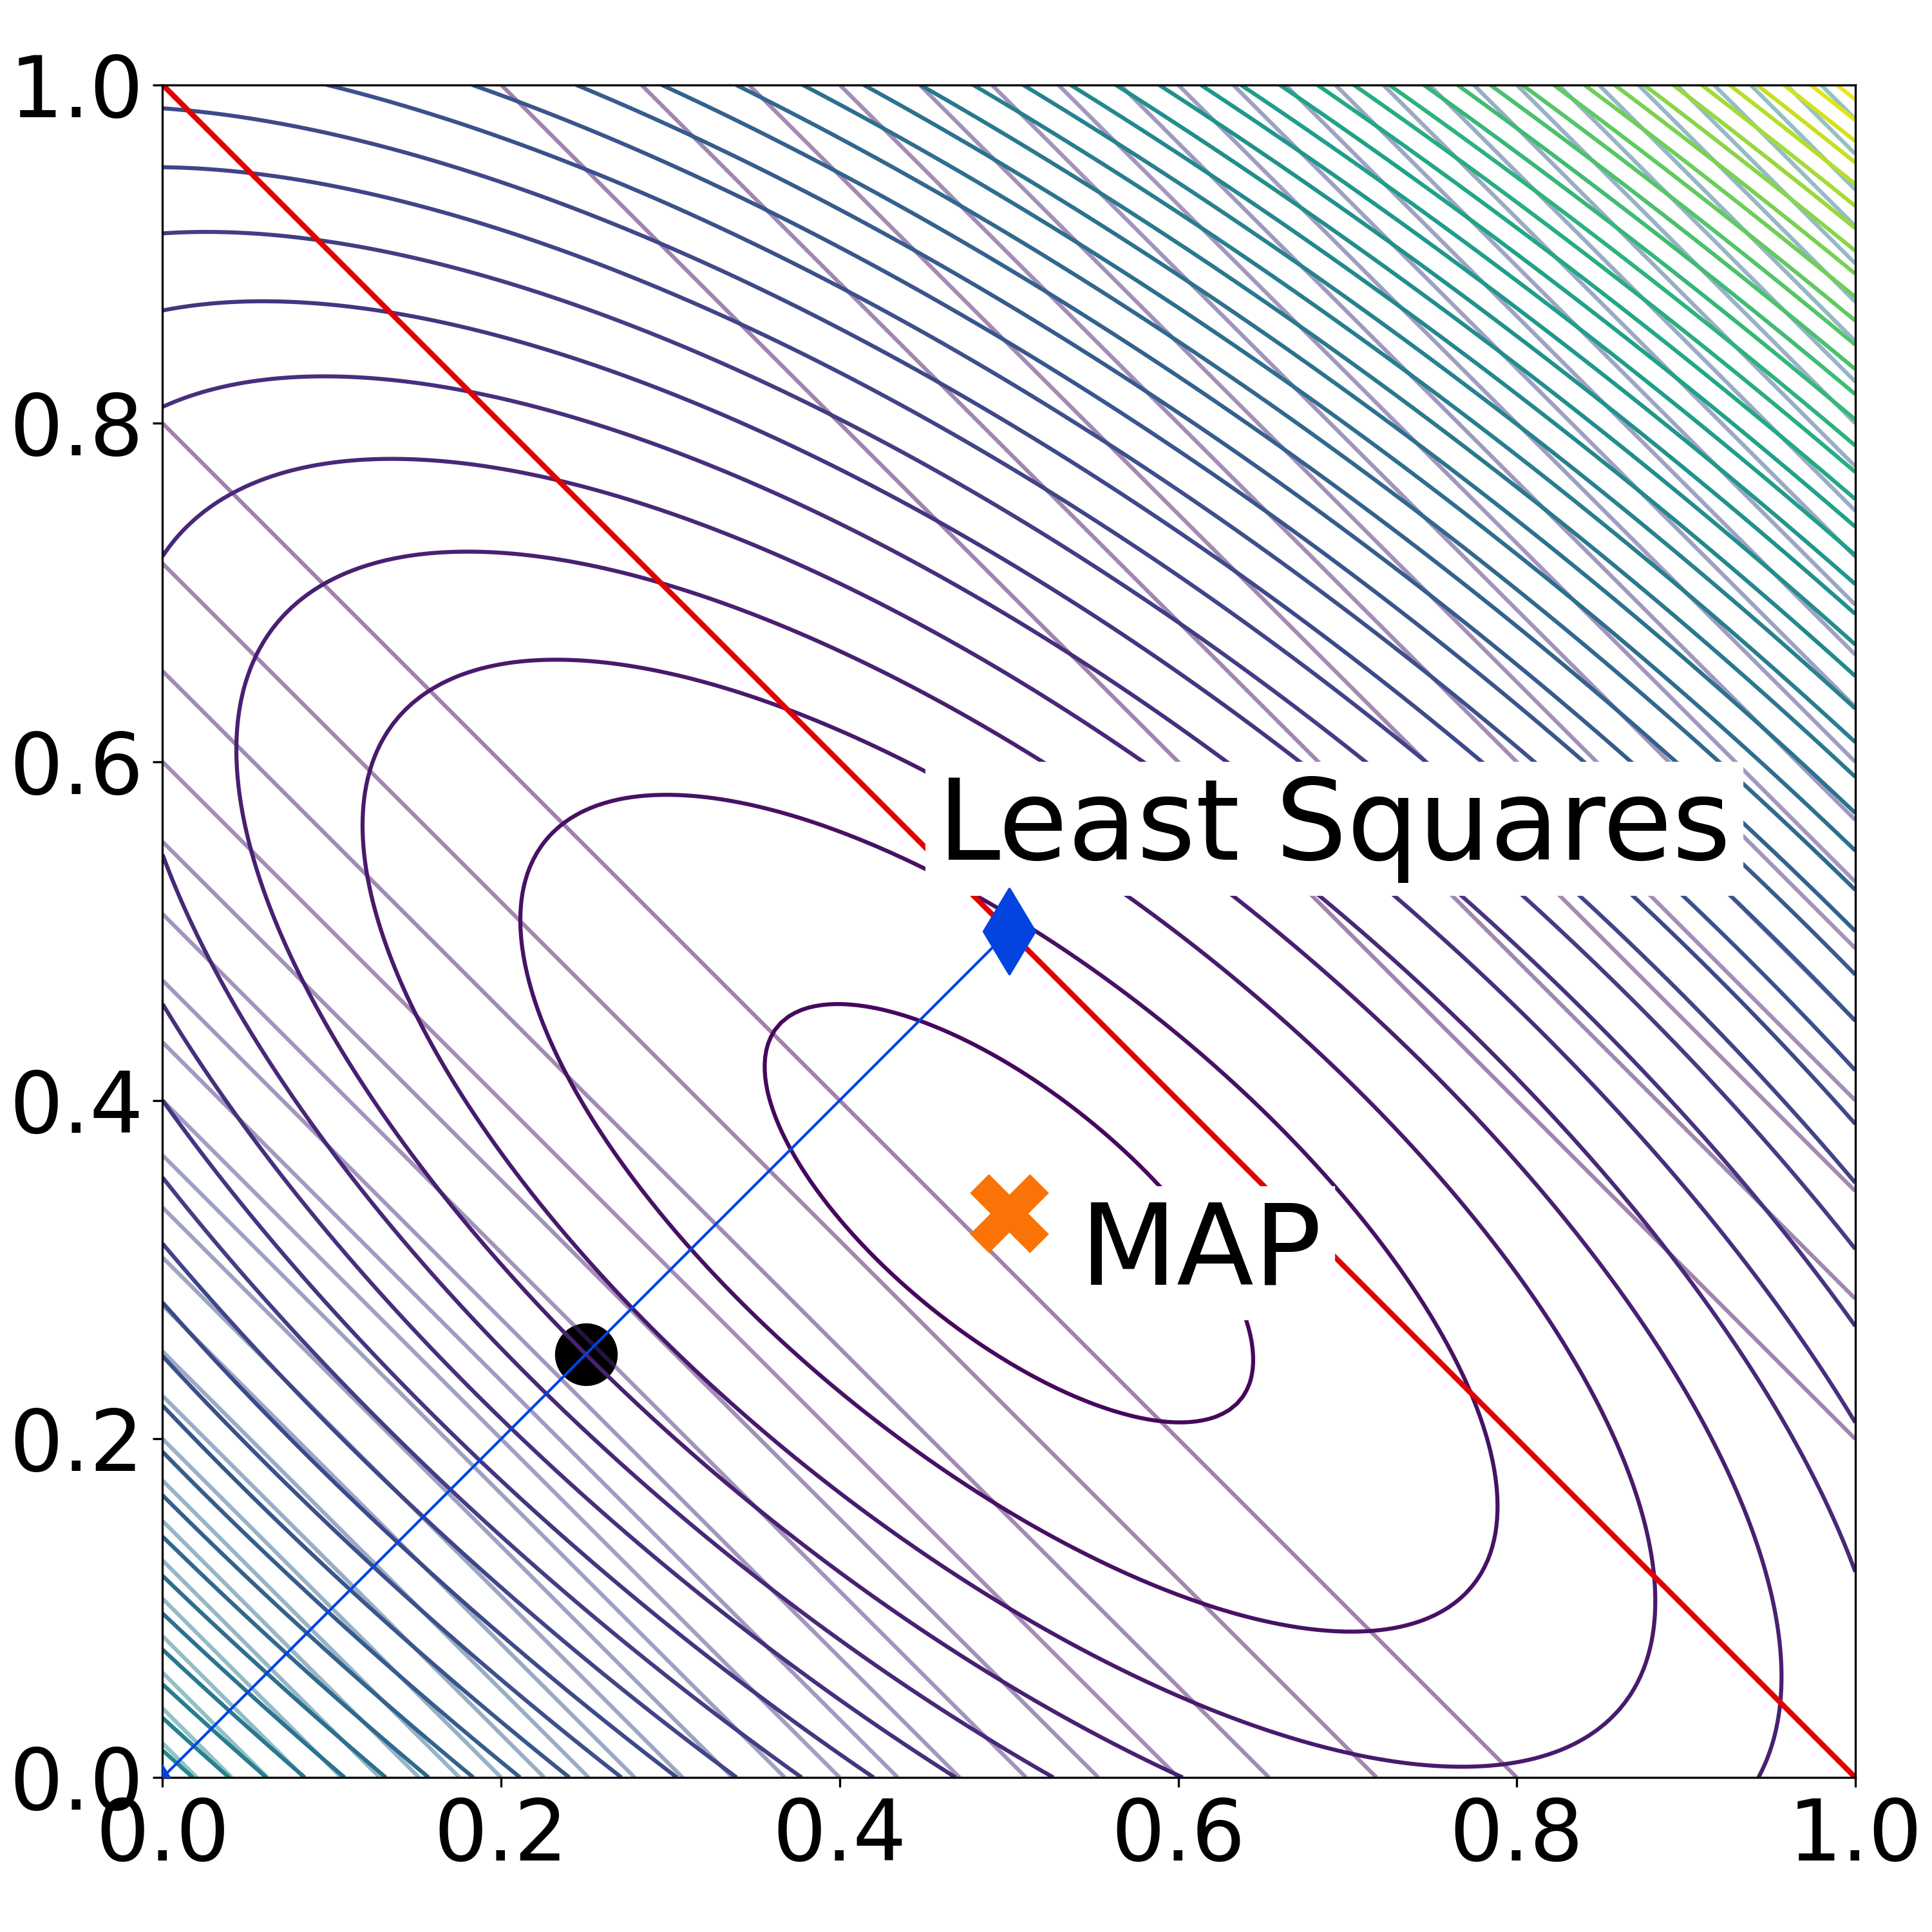
\includegraphics[width=0.25\linewidth]{figures/classical_solution.png}}
      {bayesian posterior}
    \\
    \hline
      \subf{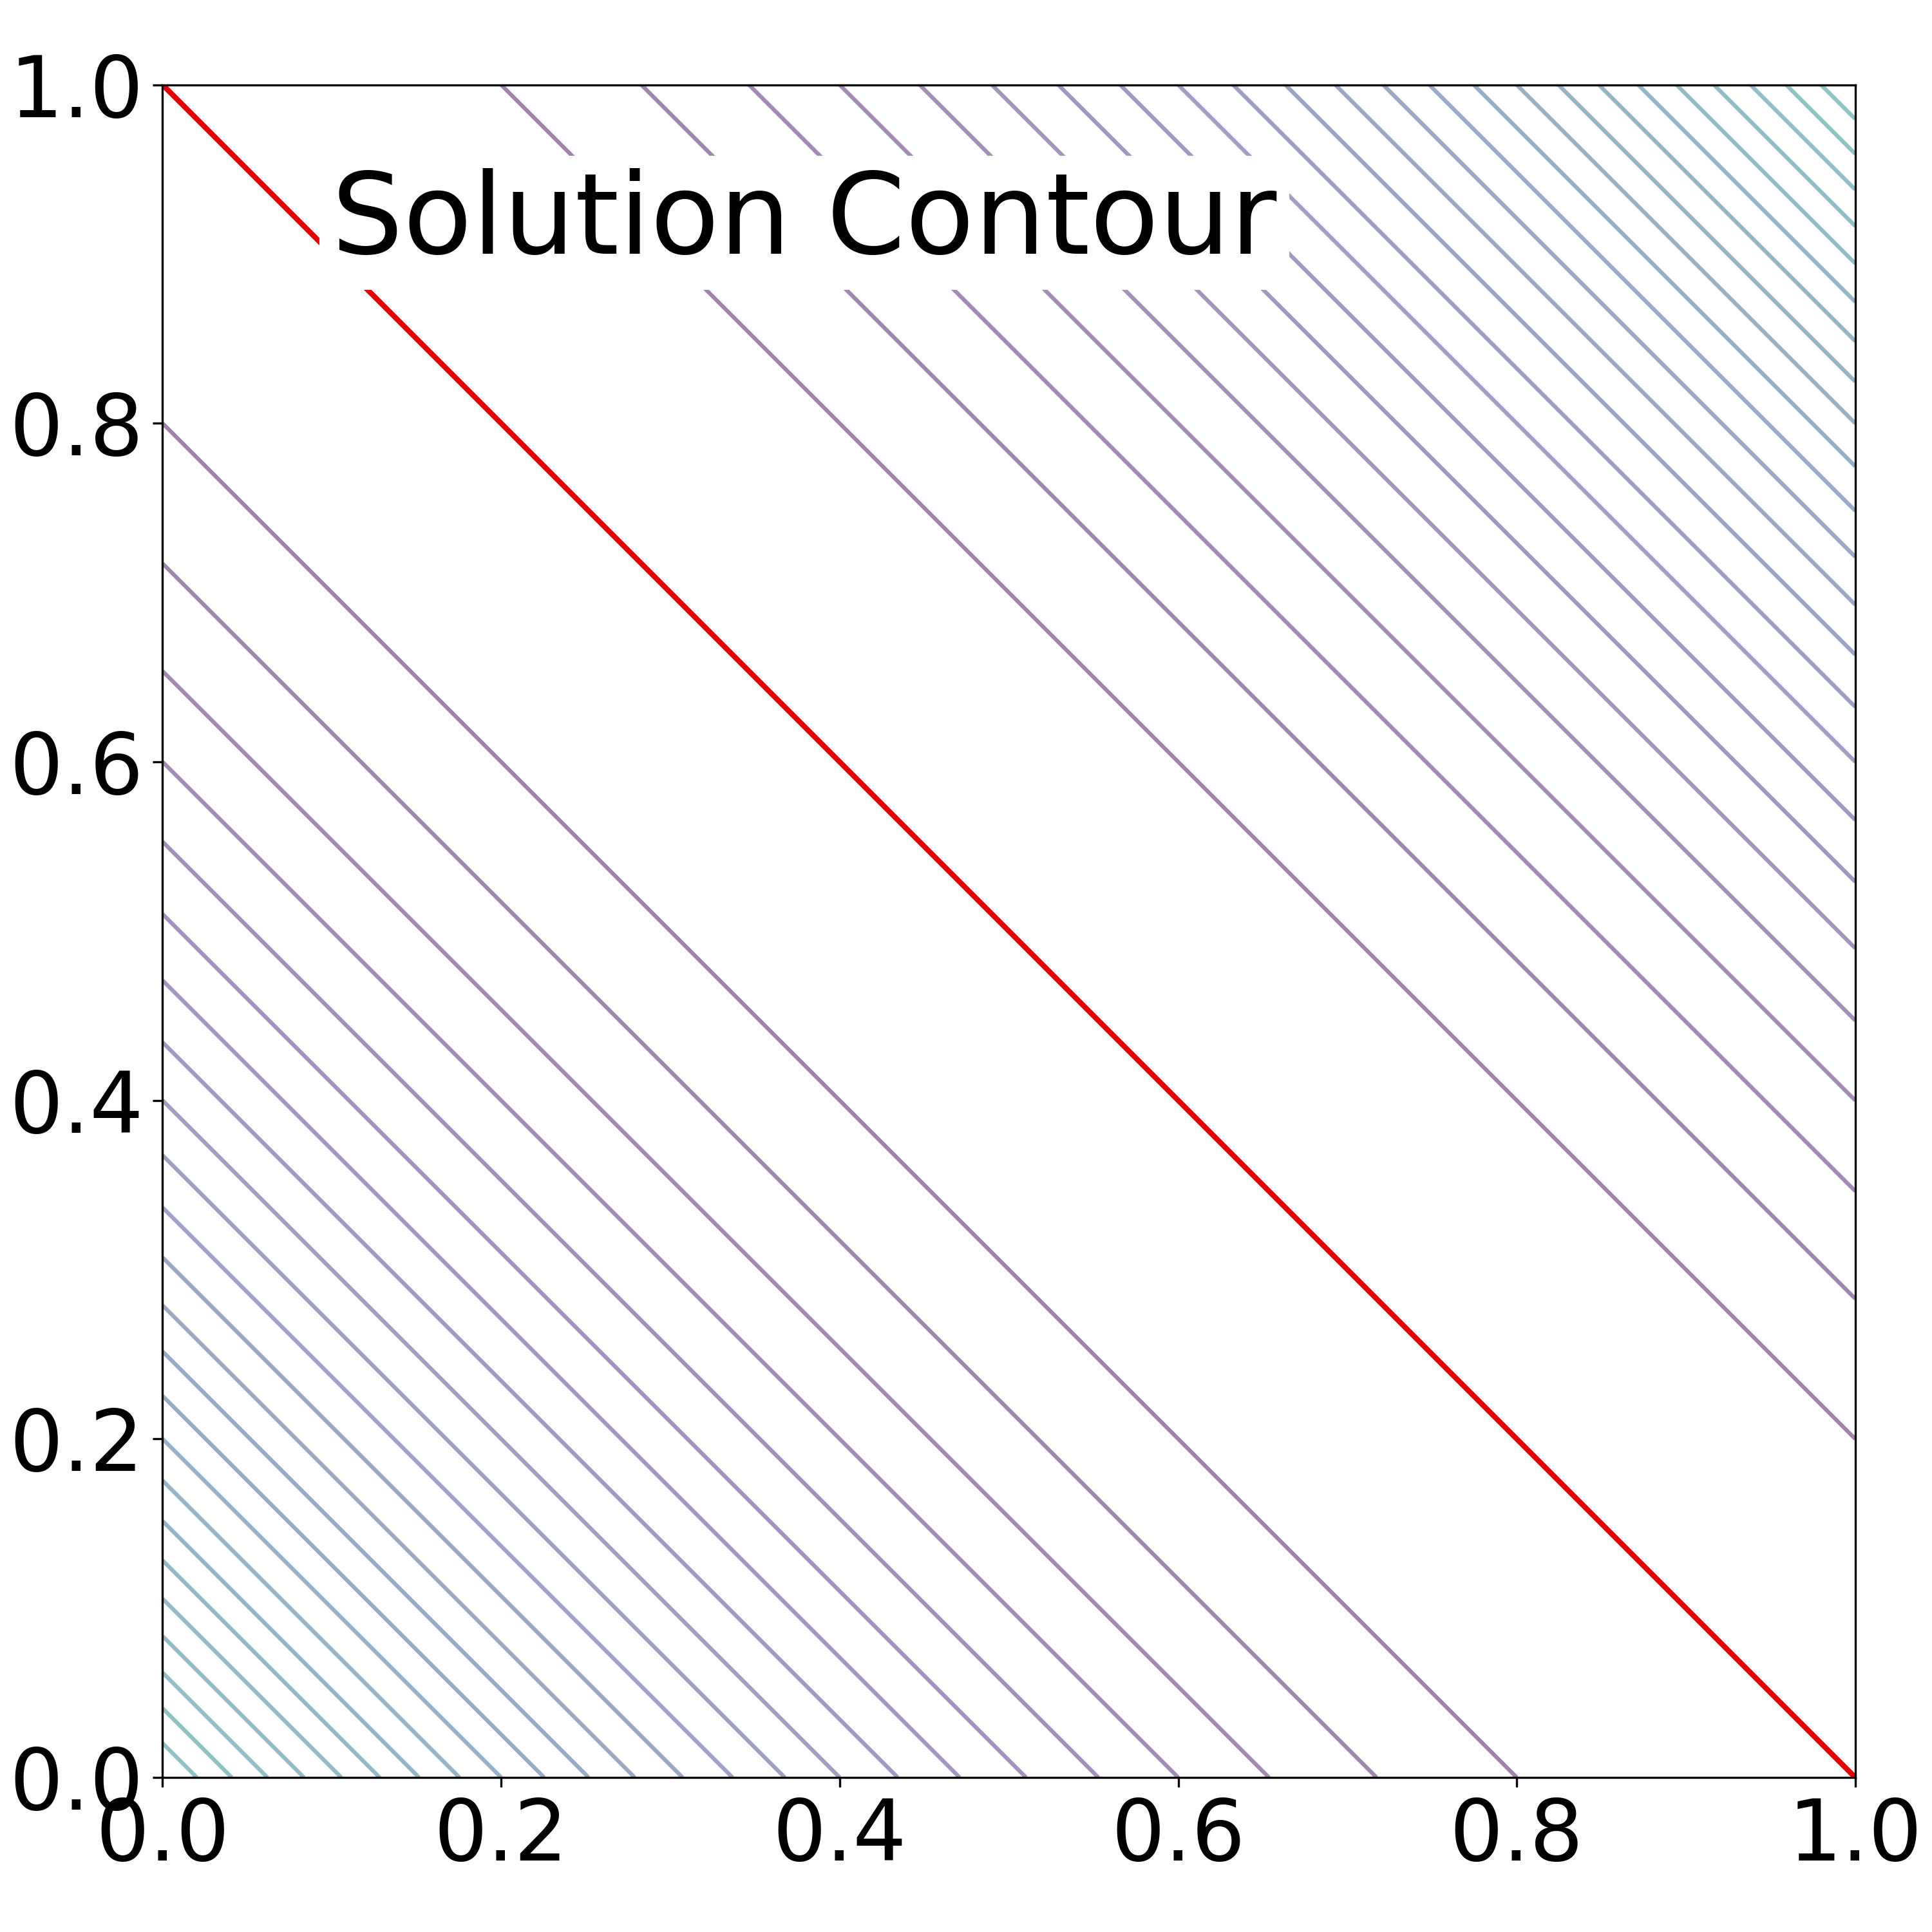
\includegraphics[width=0.25\linewidth]{figures/data_mismatch_contour.png}}
      {data mismatch}
    &
      \subf{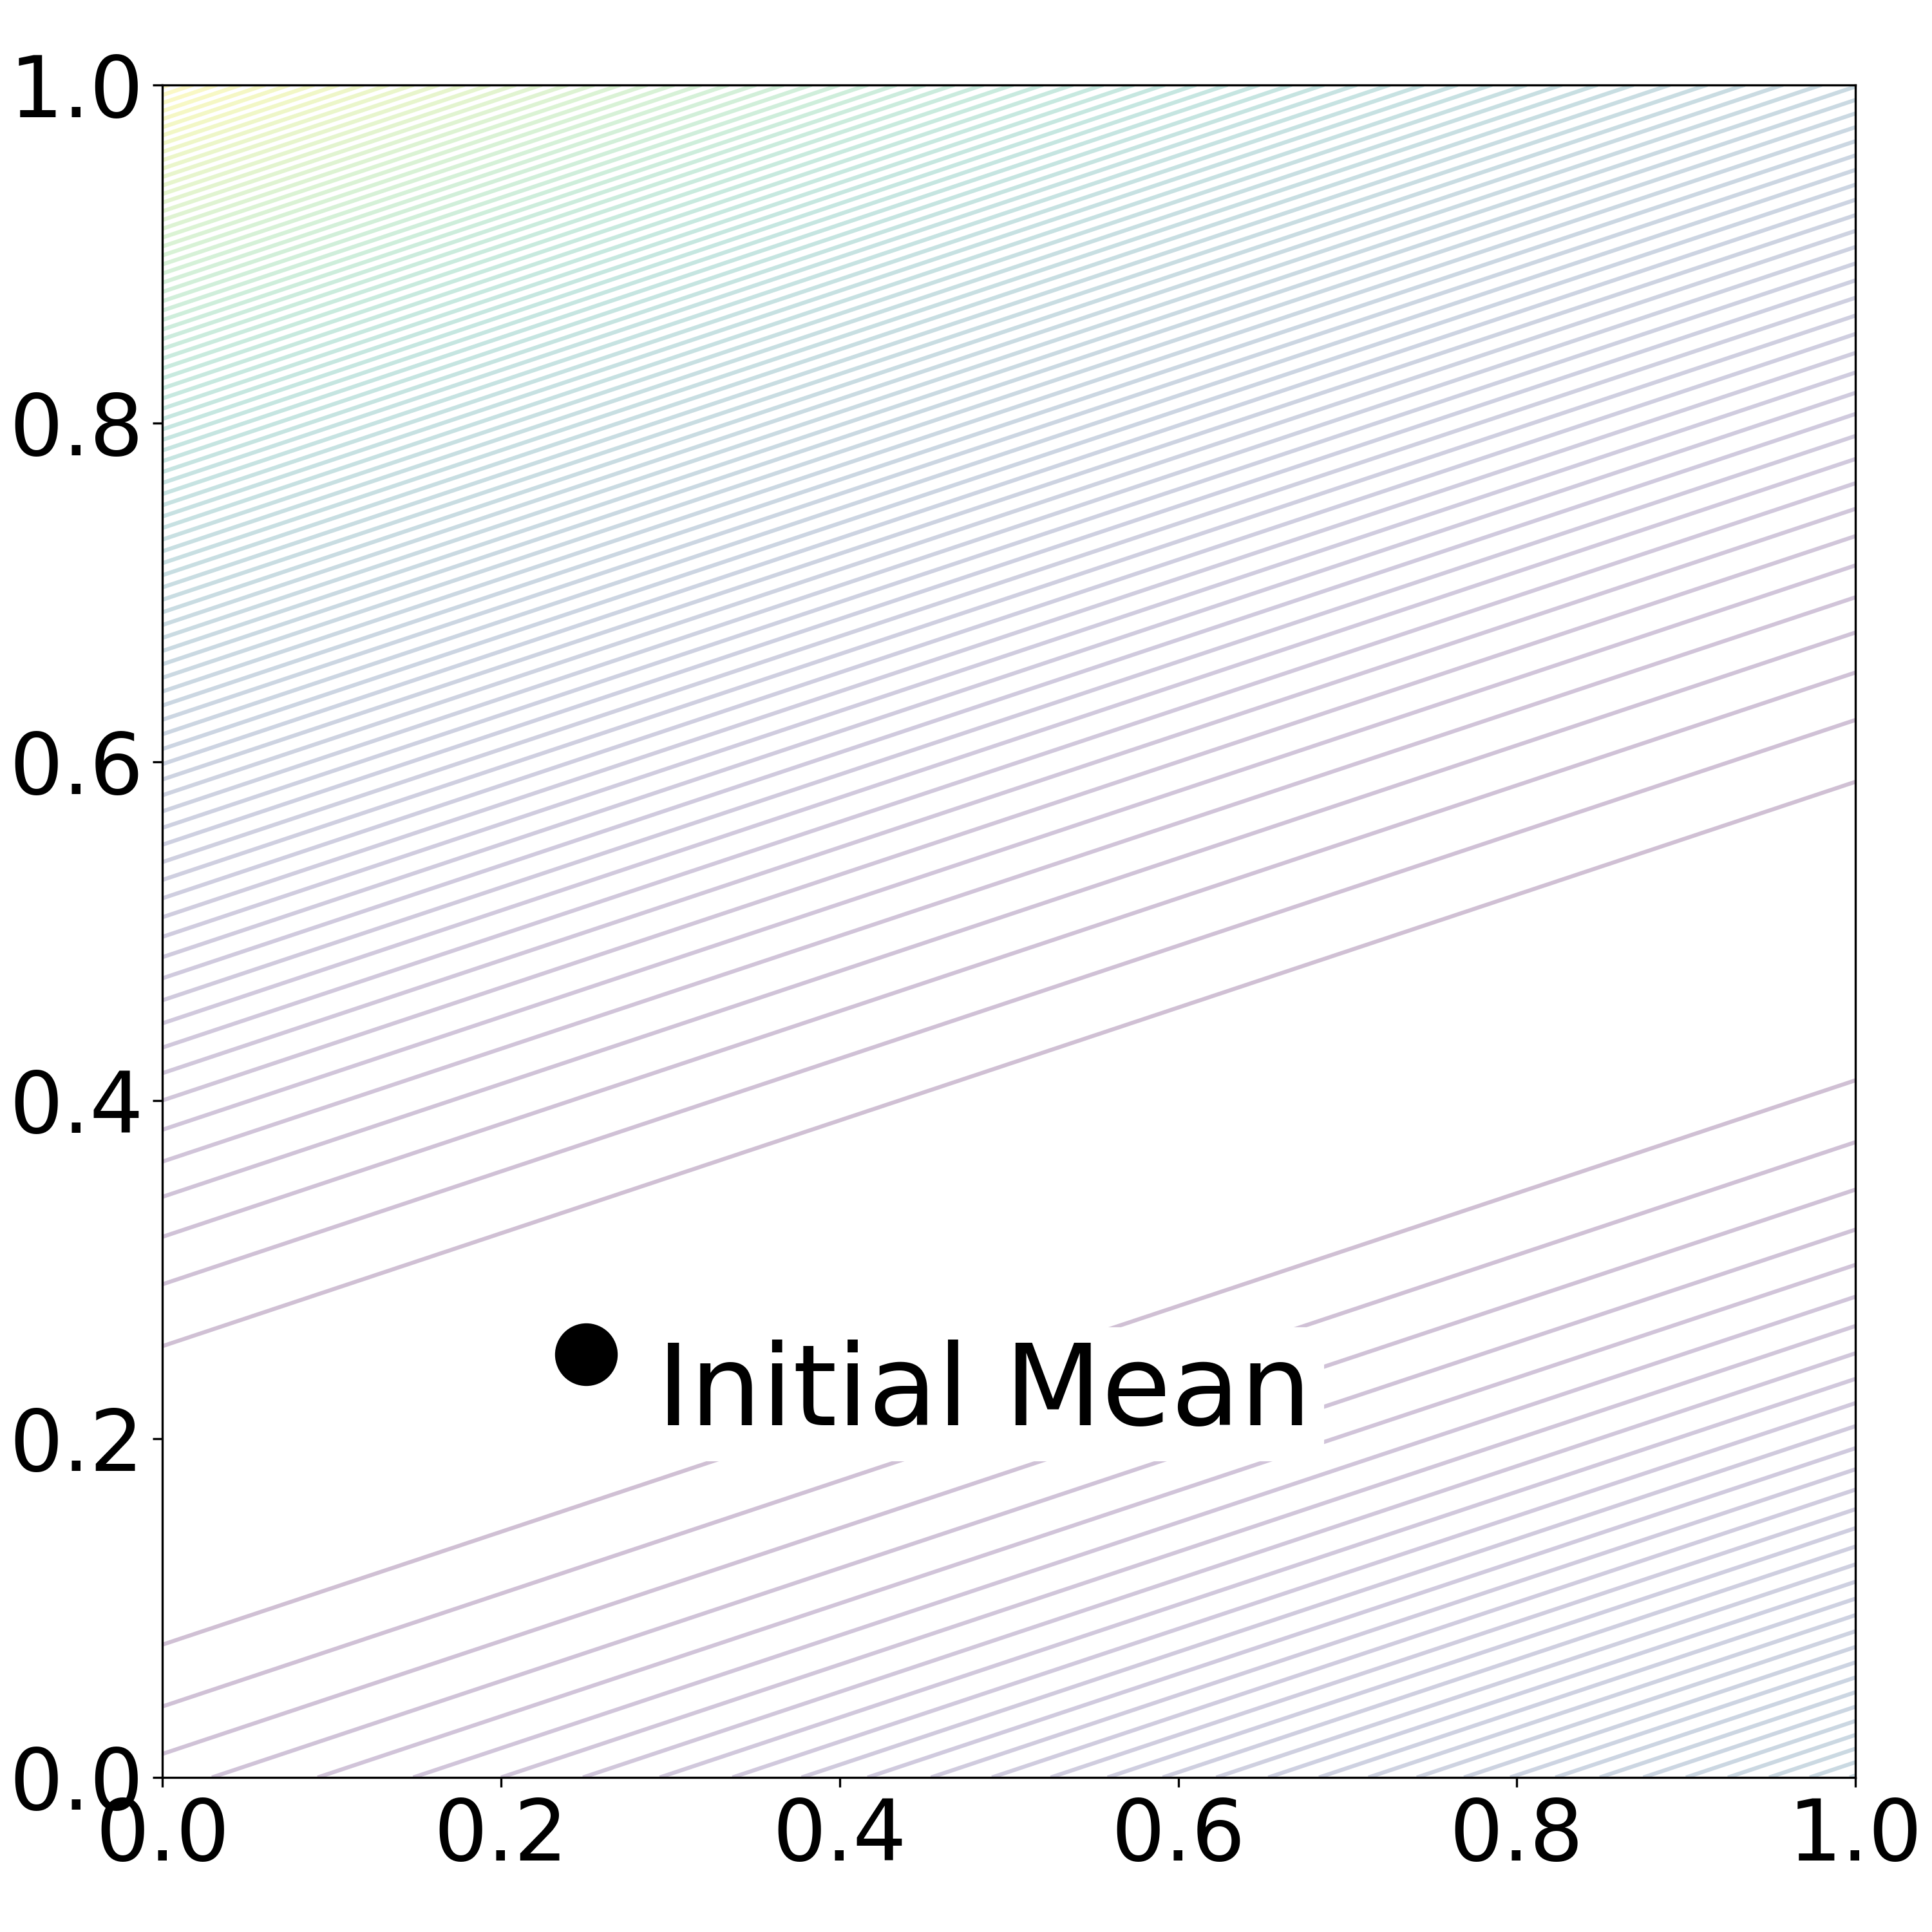
\includegraphics[width=0.25\linewidth]{figures/consistent_contour.png}}
      {modified regularization}
    &
      \subf{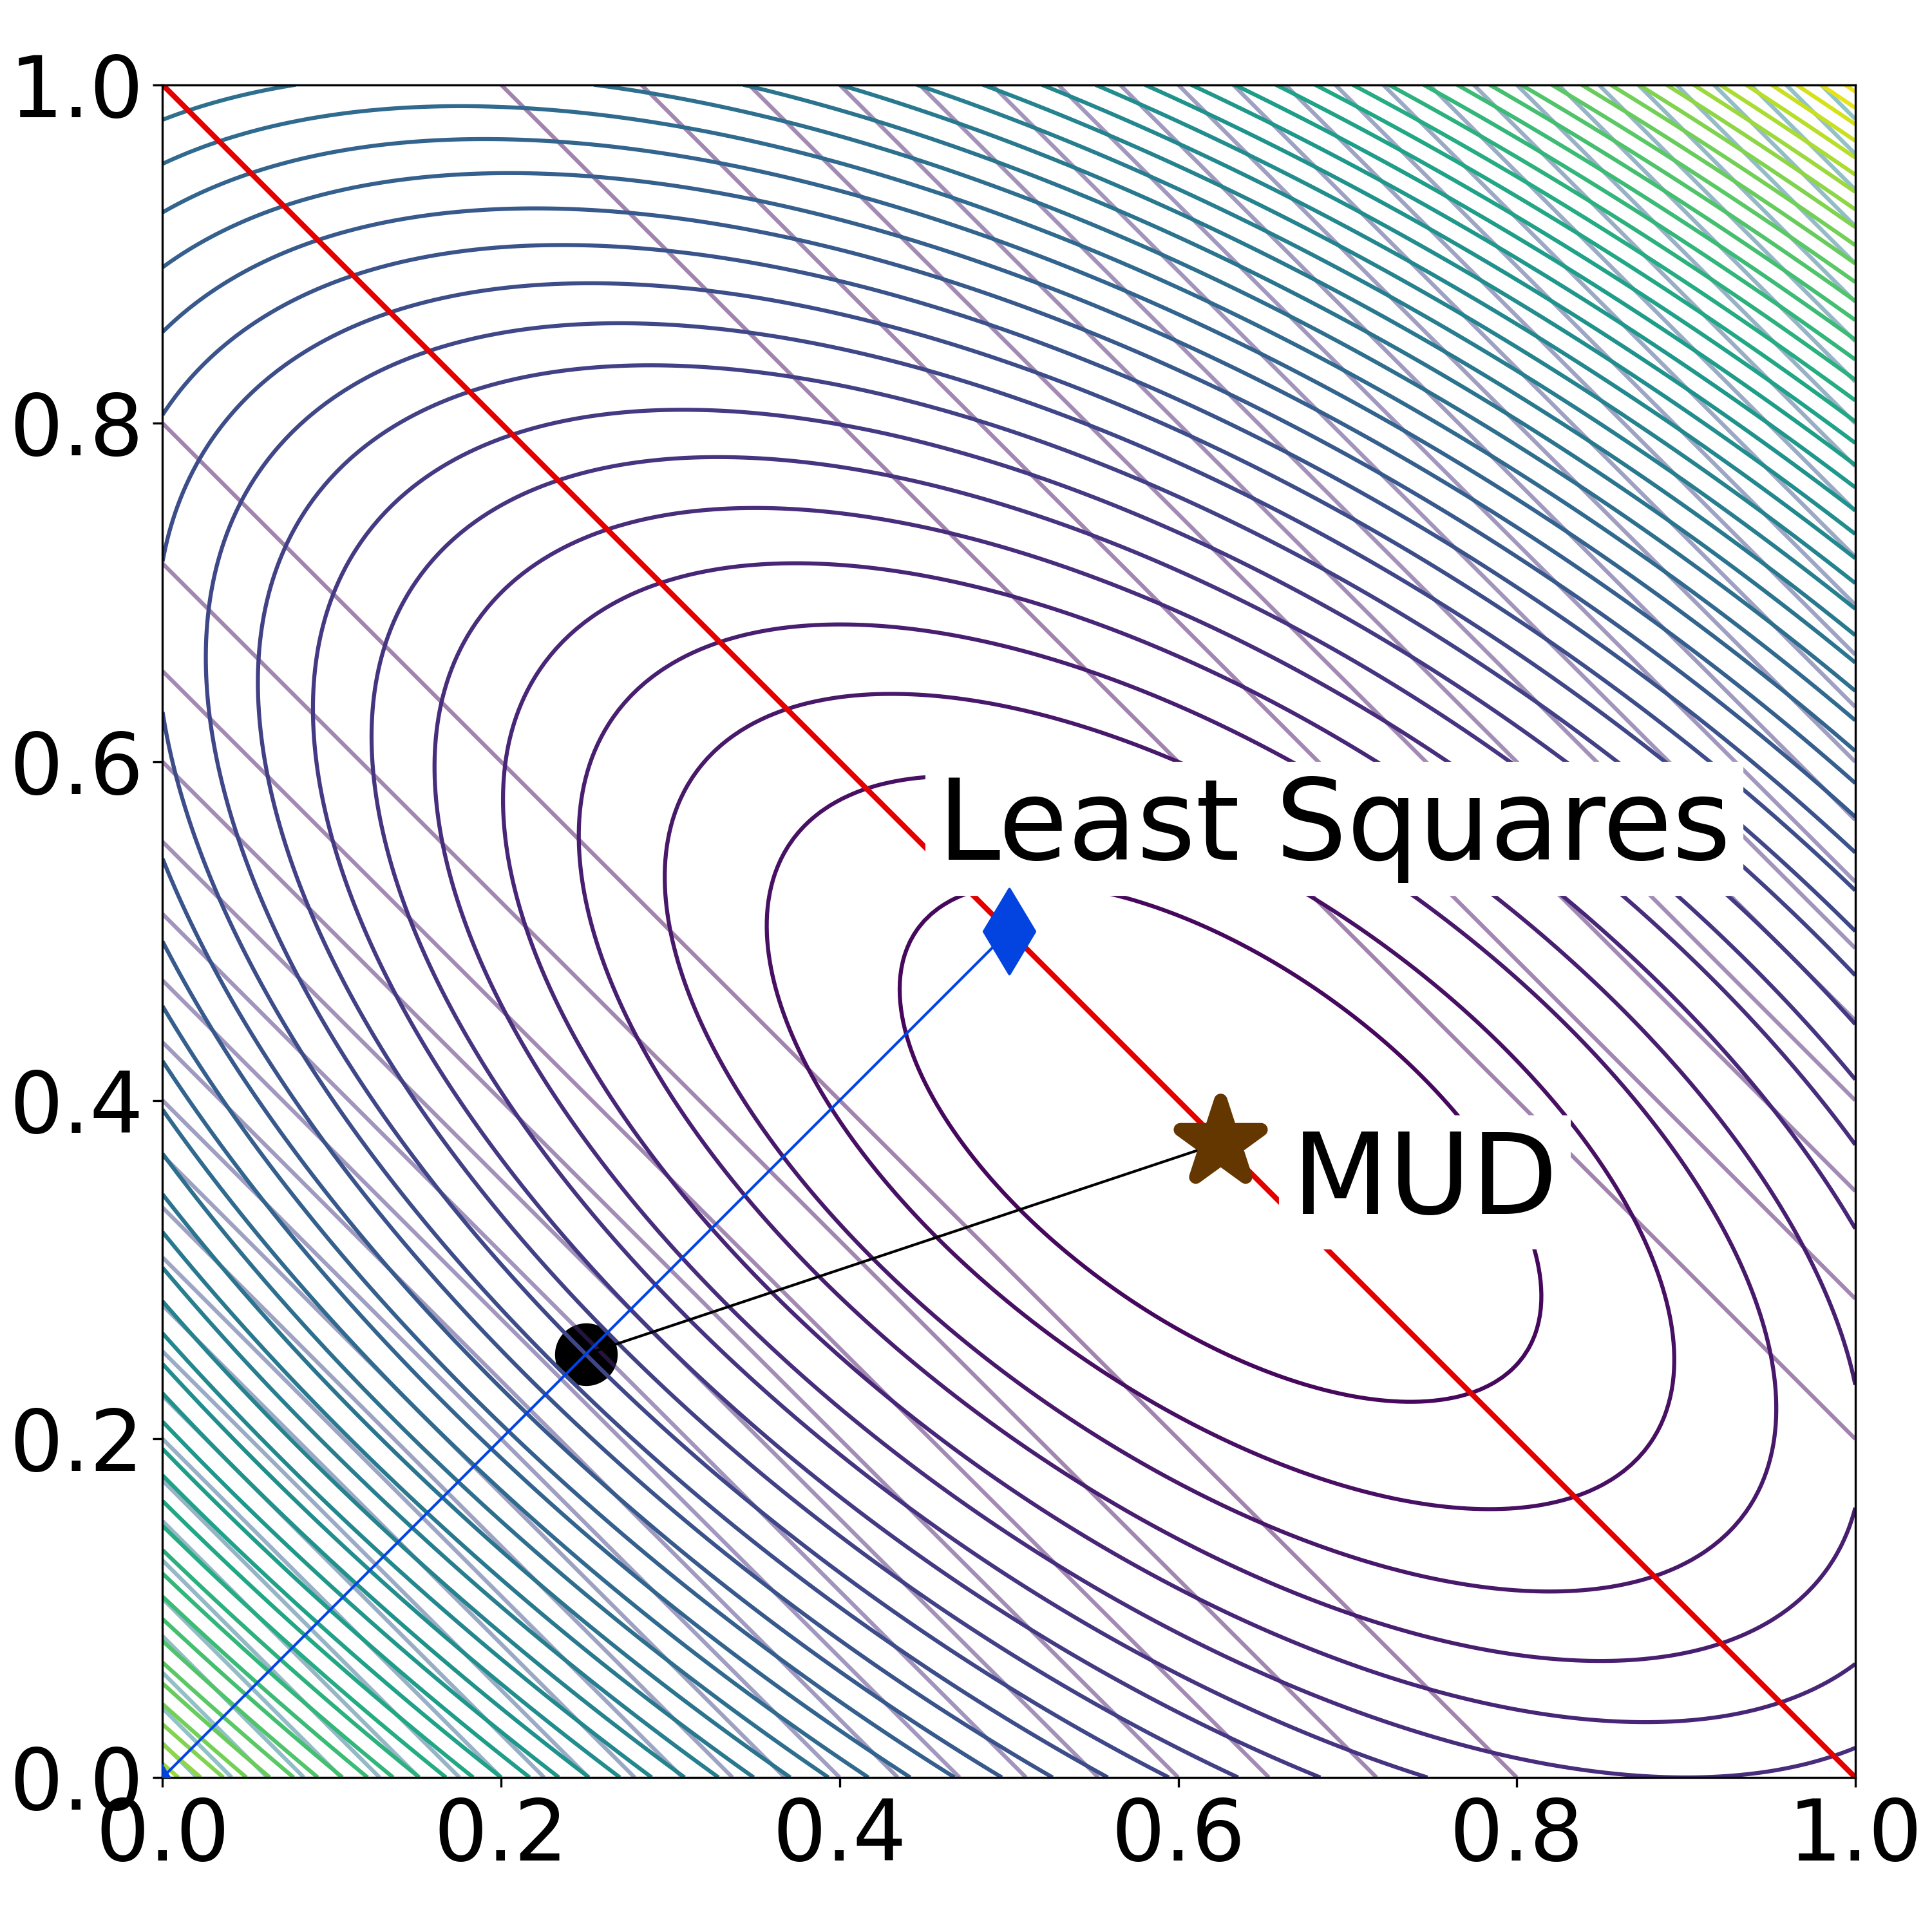
\includegraphics[width=0.25\linewidth]{figures/consistent_solution.png}}
       {updated density}
    \\
    \hline
  \end{tabular}
  %
  % \caption{Gaussian data mismatch for a 2-to-1 linear map (left plots). Gaussian initial/prior induce different regularization terms (middle plots), which leads to different optimization functions (right plots) and parameter estimates.}
  \label{fig:regularization}
\end{figure}


\end{figure}

\end{frame}


%%%%%%%%%%%%%%%%%%%%%%%%%%%%%%%%%%%%%%%%%%%%%%%%%%%%%%%%%%%
\subsection{Closed-Form Solutions}
%%%%%%%%%%%%%%%%%%%%%%%%%%%%%%%%%%%%%%%%%%%%%%%%%%%%%%%%%%%

\begin{frame}

\begin{itemize}
\item Posterior covariance:

\begin{equation}\label{eq:map_cov}
  \Sigma_\text{post} := ( A^\top {\Sigma}_\text{obs}^{-1} A + \initialCov^{-1} )^{-1}
\end{equation}

\bigskip
\item Using Woodbury identity and~\eqref{eq:predictCov}:

\begin{equation}\label{eq:map_cov_analytical}
  \Sigma_\text{post} = \initialCov - \initialCov A^\top \left[\predictedCov + \observedCov\right]^{-1} A \initialCov
\end{equation}

\bigskip
\item Interpretation: $\Sigma_\text{post}$ is a rank $d$ correction (or update) of $\initialCov$.

\bigskip
\item $\predictedCov + \observedCov$ is invertible because it is the sum of two s.p.d matrices. \\

\bigskip
\item Rewrite using analytical expression for the MAP point:

\begin{equation}\label{eq:map-point-analytical}
  \param^{\text{MAP}} = \param_0 + \Sigma_\text{post} A^\top \observedCov^{-1} (\observedMean - b - A\param_0).
\end{equation}

\end{itemize}

\end{frame}


%%%%%%%%%%%%%%%%%%%%%%%%%%%%%%%%%%%%%%%%%%%%%%%%%%%%%%%%%%%
\begin{frame}[t]{\it The one where we make some convenient manipulations.}
\begin{itemize}
  \item Let

  \begin{equation}\label{eq:eff_reg}
  	R := \nolinebreak \initialCov^{-1} - \nolinebreak A^\top \predictedCov^{-1} A.
  \end{equation}

  \bigskip
  \item Using this $R$, rewrite $J(\param)$ as

  \begin{equation}\label{eq:dci-objective-alt}
  J(\param):= \norm{\observedMean - Q(\param)}_{\observedCov^{-1}}^2 + \norm{\param - \param_0}_{R}^2.
  \end{equation}

  \bigskip
  \item $R$ is the {\em effective regularization} in $J(\param)$ in the DCI framework:

  \begin{equation}
  	\updatedCov := \left(A^\top \observedCov^{-1} A + R\right)^{-1}
  \end{equation}

  \bigskip
  \item Since $R$ is not invertible, Woodbury's identity cannot be applied (yet).

\end{itemize}

\end{frame}

%%%%%%%%%%%%%%%%%%%%%%%%%%%%%%%%%%%%%%%%%%%%%%%%%%%%%%%%%%%
\begin{frame}[t]{\it The one where we make some convenient manipulations.}
\begin{itemize}
  \item \emph{Using linear algebra ...}

  \begin{equation}\label{eq:updatedCov_final}
  	\updatedCov = \initialCov - \initialCov A^\top \predictedCov^{-1}\left[\predictedCov-\observedCov\right]\predictedCov^{-1}A\initialCov.
  \end{equation}

  \bigskip
  \bigskip
  \item Substitute $\updatedCov$ for $\Sigma_\text{post}$ in \eqref{eq:map-point-analytical}:

  \begin{equation}\label{eq:mud-point-analytical-alt}
  \param^{\text{MUD}} = \param_0 + \updatedCov A^\top \observedCov^{-1} (\observedMean - b - A\param_0).
  \end{equation}

  \bigskip
  \bigskip
  \item Substituting~\eqref{eq:updatedCov_final} into~\eqref{eq:mud-point-analytical-alt} and simplifying, we have

  \begin{equation}\label{eq:mud-point-analytical-final}
  	\mudpt = \param_0 + \initialCov A^\top \predictedCov^{-1}(\observedMean - b - A\param_0).
  \end{equation}

\end{itemize}

\end{frame}

%%%%%%%%%%%%%%%%%%%%%%%%%%%%%%%%%%%%%%%%%%%%%%%%%%%%%%%%%%%
\begin{frame}

\begin{thm}\label{thm:MUD_existence_uniqueness}

Suppose  $Q(\param)=A\param+b$ for some full rank $A\in\RR^{d\times p}$ with $d\leq p$ and $b\in\RR^d$.

If $\initial \sim N(\param_0,\initialCov)$, $\observed\sim N(\observedMean,\observedCov)$, and the predictability assumption holds, then

\begin{enumerate}[(a)]
  \item There exists a unique $\mudpt$.
  \item $Q(\mudpt) = \observedMean$.
  \item If $d=p$, $\mudpt$ is given by $A^{-1}$. If $d<p$, $\mudpt$ is given by~\eqref{eq:mud-point-analytical-final} and the covariance associated with this point is given by~\eqref{eq:updatedCov_final}.
\end{enumerate}
\end{thm}

\end{frame}

%%%%%%%%%%%%%%%%%%%%%%%%%%%%%%%%%%%%%%%%%%%%%%%%%%%%%%%%%%%
\begin{frame}{\it The one where we address a key assumption}

\begin{itemize}
  \item Predictability Assumption: $\predicted$ is a dominating measure for $\observed$
  \bigskip
  \bigskip
  \item Linear case: involves eigenvalues of covariances:
  \bigskip
    \begin{itemize}
      \item min eigenvalue $\predictedCov$ > max eigenvalue $\observedCov$
    \end{itemize}
\end{itemize}
\end{frame}

%%%%%%%%%%%%%%%%%%%%%%%%%%%%%%%%%%%%%%%%%%%%%%%%%%%%%%%%%%%
\subsection{Impact of Information Content}
%%%%%%%%%%%%%%%%%%%%%%%%%%%%%%%%%%%%%%%%%%%%%%%%%%%%%%%%%%%

\begin{frame}{\it The one where we show how rank and dimension impact our solutions.}
\centering

\begin{figure}[htbp]
\hbox{
  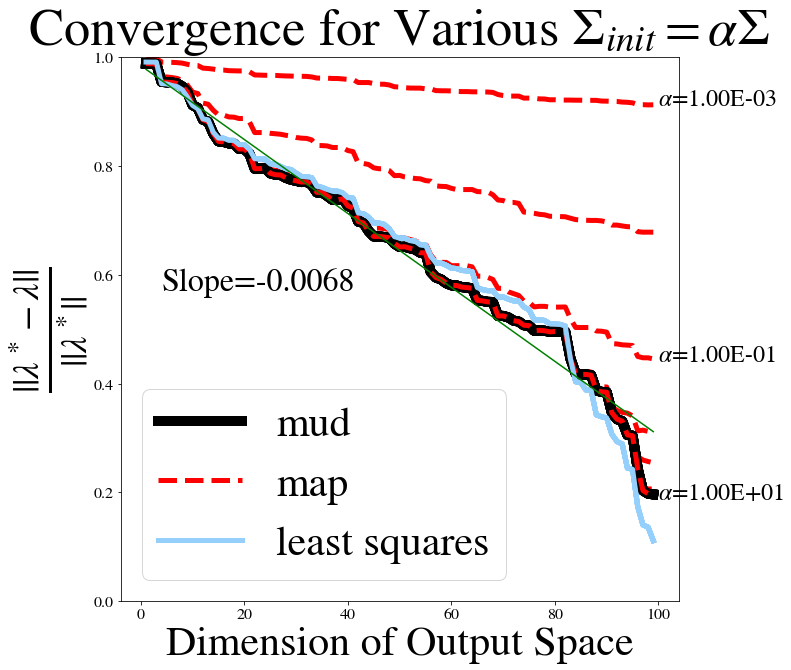
\includegraphics[width=0.5\linewidth]{figures/lin/lin-dim-cov-convergence}
  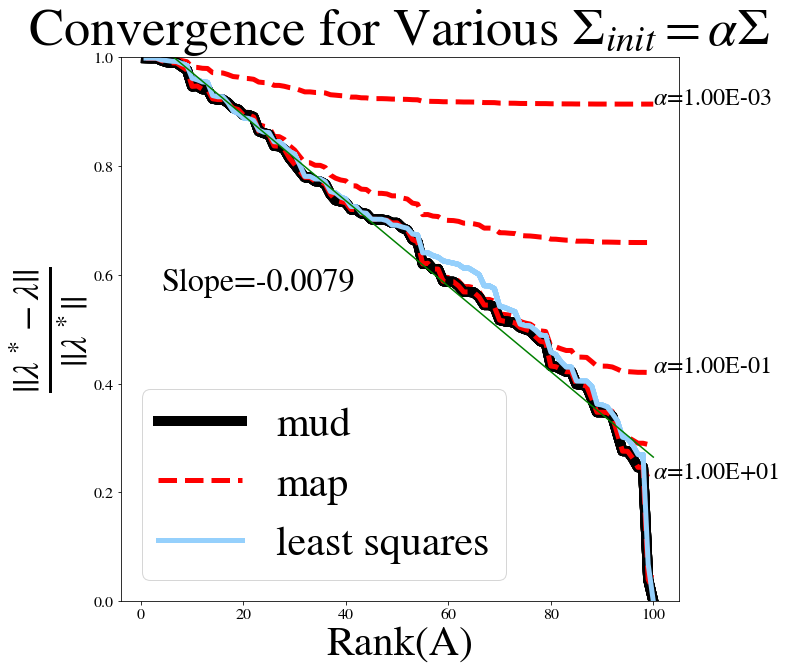
\includegraphics[width=0.5\linewidth]{figures/lin/lin-rank-cov-convergence}
}
% \caption{
% 	Relative errors between $\paramref$ and (i) the least squares solution obtained through {\tt numpy}'s {\tt linalg.pinv} module, (ii) the closed-form solution for the MUD point given in Eq~\eqref{eq:mud-point-analytical-final}, and (iii) the MAP point.
%   (Left): Error for increasing dimensions of $D$ for $A$ taken to be a Gaussian Random Map.
%   (Right): Error for increasing row-rank of $A$, generated with Gaussian vectors and a SVD.
% }
\label{fig:lin-error}
\end{figure}

Example: scaling random diagonal initial covariances

\end{frame}


%%%%%%%%%%%%%%%%%%%%%%%%%%%%%%%%%%%%%%%%%%%%%%%%%%%%%%%%%%%
\subsection{Data-Driven QoI Maps}
%%%%%%%%%%%%%%%%%%%%%%%%%%%%%%%%%%%%%%%%%%%%%%%%%%%%%%%%%%%

\begin{frame}{\it The one where we leverage this framework for general streams of data.}

\begin{itemize}
  \item Measurement devices $M_j$ generating repeated noisy data, $1\leq j\leq d$.

  \bigskip
  \item $d_{j,i}$ is the $i$th noisy datum for the $j$th measurement, where $1\leq i\leq N_j$.

  \bigskip
  \item Unbiased additive error model for the measurement noise:

  \begin{equation}\label{eq:obs_data_error}
  	d_{j,i} = M_j(\paramref) + \xi_i, \ \xi_i\sim N(0,\sigma_j^2), \ \ 1\leq i\leq N_j.
  \end{equation}

\end{itemize}

\bigskip
\bigskip
\centering
{\it We now construct a $d$-dimensional vector-valued map from data obtained on the $d$ measurement devices.}

\end{frame}


%%%%%%%%%%%%%%%%%%%%%%%%%%%%%%%%%%%%%%%%%%%%%%%%%%%%%%%%%%%
\begin{frame}{\it The one with the Weighted Mean Error (WME) map $Q_\text{WME}(\param)$.}

\begin{equation}\label{eq:qoi_WME}
	Q_{\text{WME},j}(\param) := \frac{1}{\sqrt{N_j}} \sum_{i=1}^{N_j} \frac{M_j(\param)-d_{j,i}}{\sigma_j}.
\end{equation}

\bigskip
\begin{itemize}
  \item $Q_{\text{WME},j}(\paramref)$ is the sample avg of $N_j$ draws from an i.i.d.~$N(0,N_j)$.

  \bigskip
  \item Observed data are generated according to fixed (truth) $\paramref$ in \eqref{eq:obs_data_error}.

  \bigskip
  \item For each component, $Q_{\text{WME},j}(\paramref) \sim N(0, 1)$.

  \bigskip
  \item $\observed$ is a $N(\mathbf{0}_{d\times 1},\mathbf{I}_{d\times d})$ due to the structure of $Q_\text{WME}(\param)$.

\end{itemize}


\end{frame}

%%%%%%%%%%%%%%%%%%%%%%%%%%%%%%%%%%%%%%%%%%%%%%%%%%%%%%%%%%%
\begin{frame}{\it The one where measurements impact the predictability assumption.}

\begin{itemize}

	\item The $j$th diagonal component of $\predictedCov$ is given by the predicted variance associated with using the scalar-valued $Q_{\text{WME},j}$.

	\bigskip
  \item The associated predicted variance for the $j$th component is given by:

	\bigskip
  \begin{equation}
  	\frac{N_j}{\sigma_j^2} M_j\initialCov M_j^\top.
  \end{equation}

  \bigskip
  \item $\initialCov$ non-degenerative and $M_j$ non-trivial row vector, which implies that the {\it \bf predicted variance grows linearly} with $N_j$.\\

\end{itemize}

\bigskip
\bigskip
\centering
{\it The following result is now an immediate consequence of Theorem~\ref{thm:MUD_existence_uniqueness}.}
\end{frame}

%%%%%%%%%%%%%%%%%%%%%%%%%%%%%%%%%%%%%%%%%%%%%%%%%%%%%%%%%%%
\begin{frame}

\begin{corollary}\label{cor:MUD_wme}
If $\initial \sim N(\param_0,\initialCov)$ and data are obtained for $d$ linearly independent measurements on $\pspace$ with an additive noise model with i.i.d. Gaussian noise for each measurement, then {\bf there exists a minimum number of data points obtained for each of the measurements} such that there exists a unique $\mudpt$ and $Q_\text{WME}(\mudpt) = 0$.
\end{corollary}

\end{frame}



%%%%%%%%%%%%%%%%%%%%%%%%%%%%%%%%%%%%%%%%%%%%%%%%%%%%%%%%%%%
\subsection{Nonlinear Examples}
%%%%%%%%%%%%%%%%%%%%%%%%%%%%%%%%%%%%%%%%%%%%%%%%%%%%%%%%%%%

%%%%%%%%%%%%%%%%%%%%%%%%%%%%%%%%%%%%%%%%%%%%%%%%%%%%%%%%%%%
\begin{frame}{\it The one where we violate some assumptions (and see what happens).}
%\vskip 25pt

Consider the exponential decay problem with uncertain decay rate $\param$:

\bigskip
$$
\begin{cases}
\frac{\partial u}{\partial t} & = \param u(t), \ 0<t\leq 3, \\ u(0) &= 0.75,
\end{cases}
$$

\bigskip
\bigskip
with solution

\begin{equation}
u(t;\param) = u_0\exp(-\param t), \; u_0 = 0.75 ,
\end{equation}

\bigskip
and measurements occur from $t=1$ until $t=3$ at rate of $100$Hz.
\end{frame}


%%%%%%%%%%%%%%%%%%%%%%%%%%%%%%%%%%%%%%%%%%%%%%%%%%%%%%%%%%%
\begin{frame}
\centering
\only<1>{
\begin{figure}[htb]
  \hbox{
		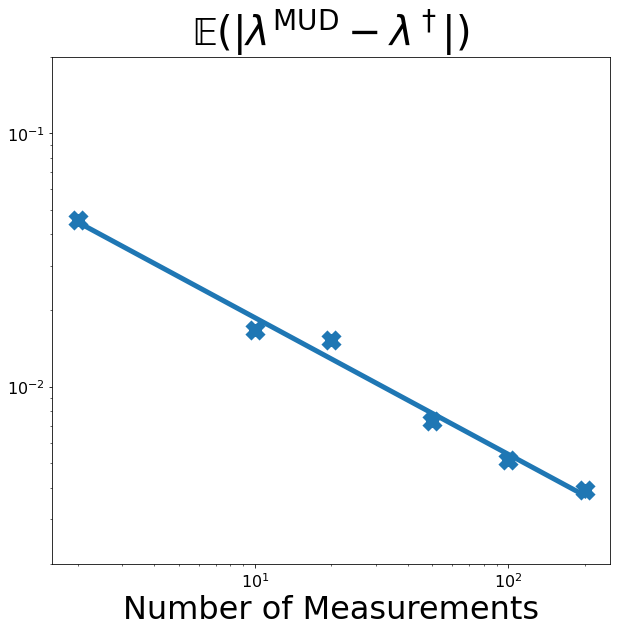
\includegraphics[width=0.45\linewidth]{figures/ode/ode_convergence_mud_obs_mean.png}
			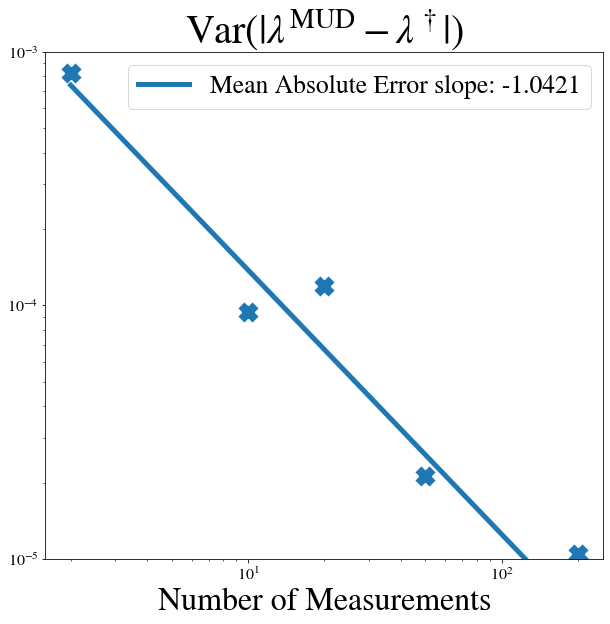
\includegraphics[width=0.45\linewidth]{figures/ode/ode_convergence_mud_obs_var.png}
	}
 %  \caption{Curves for exponential decay model with various decay coefficients. Dashed curves denote 99\% probability intervals for noise. The true signal is shown in solid black.
 % Curves associated with the MUD estimates for the decay coefficient computed from 20 trials are shown in light red.
 % Both sets of these curves encompass the true signal for $N=20$ (top plot) and $N=200$ (bottom plot) data points.
 % The light red curves are almost indistinguishable in the bottom plot as they all lie nearly on the true signal which demonstrates the overall reduction in variance in MUD estimates around the true signal when using $N=200$ data points.
 %  }
  \label{fig:ode-reference}
\end{figure}
}

\only<2>{
\begin{figure}[htb]
	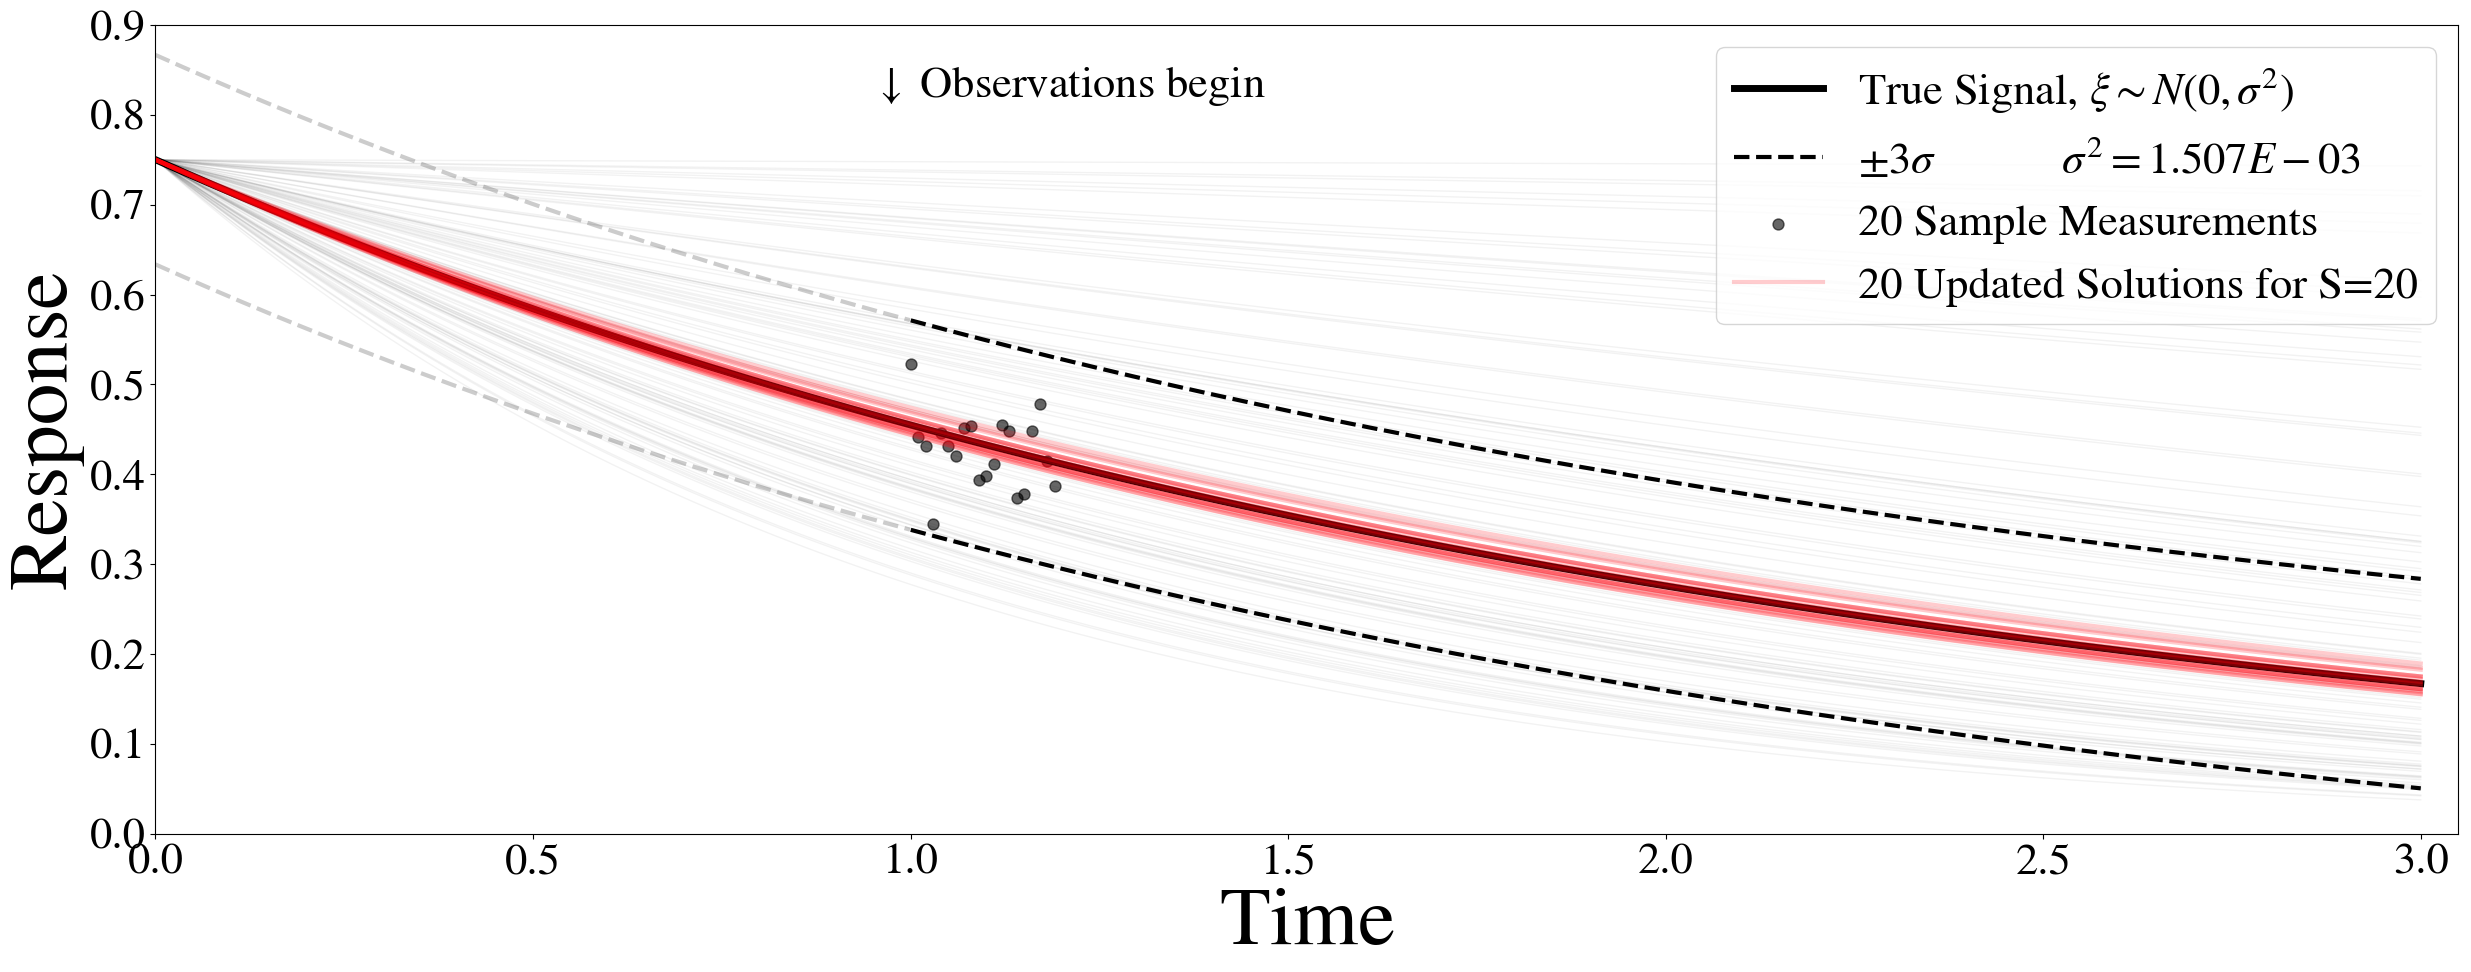
\includegraphics[width=0.85\linewidth]{figures/ode/ode_20_reference_solution.png}
	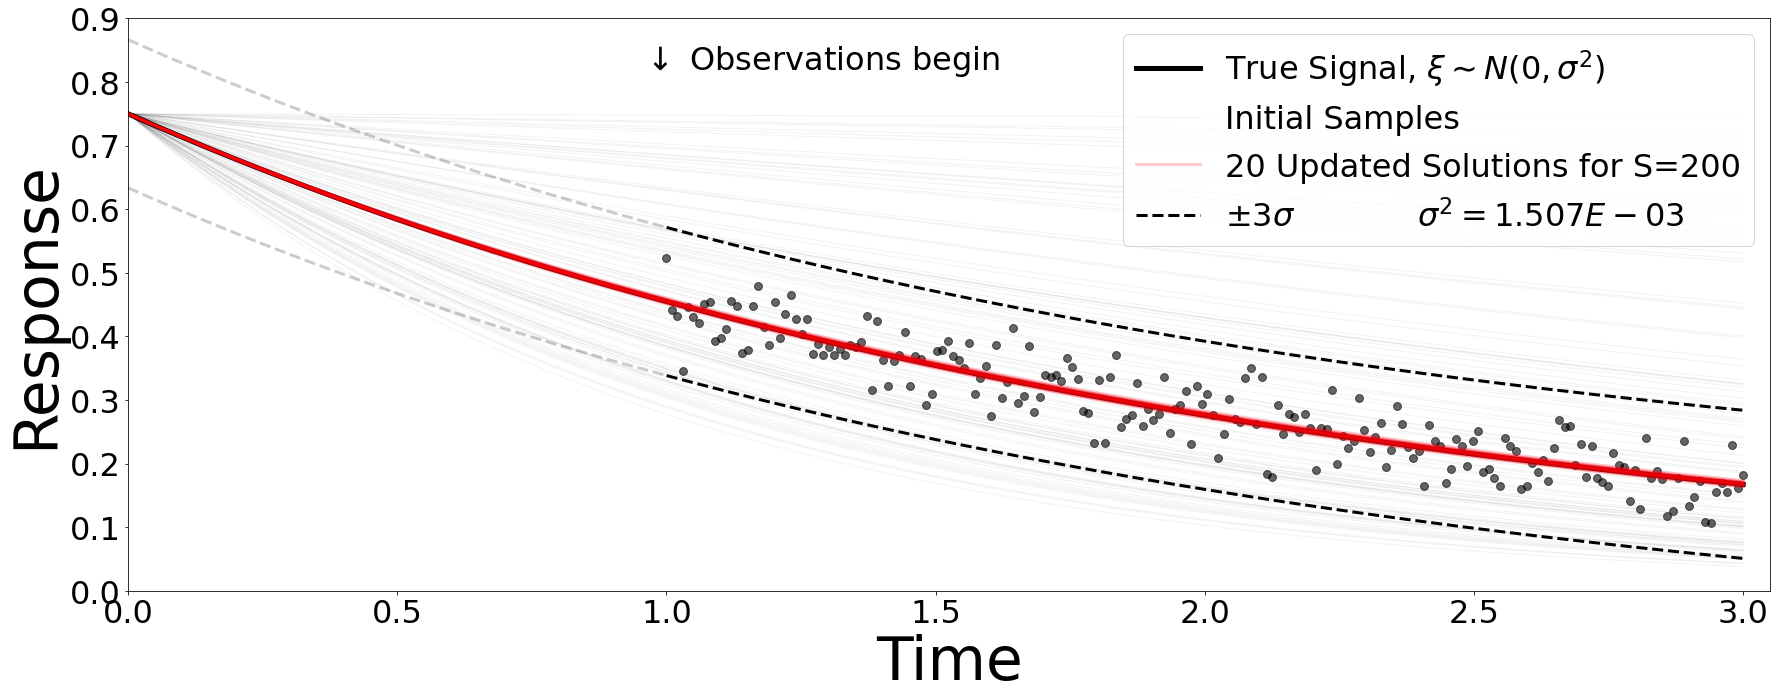
\includegraphics[width=0.85\linewidth]{figures/ode/ode_200_reference_solution.png}
  % \caption{The mean (left) and variance (right) of absolute errors in MUD estimates as a function of the number of data points used. These statistics are computed over 20 trials.
  % }
  \label{fig:ode-convergence}
\end{figure}
}

\end{frame}


%%%%%%%%%%%%%%%%%%%%%%%%%%%%%%%%%%%%%%%%%%%%%%%%%%%%%%%%%%%
\begin{frame}{\it The one where we violate some assumptions (and see what happens).}

Consider the Poisson problem:
\begin{equation}\label{eq:pde-equation}
\begin{cases}
\hfill -\nabla \cdot \nabla u &= f(x), \quad\text{on } x\in \Omega, \\
\hfill u &= 0, \quad\text{ on } \Gamma_T \cup \Gamma_B, \\
\hfill \frac{\partial u}{\partial \mathbf{n}} &= g(x_2), \quad\text{ on } \Gamma_L, \\
\hfill \frac{\partial u}{\partial \mathbf{n}} &= 0, \quad\text{ on } \Gamma_R,
\end{cases}
\end{equation}
where $x=(x_1, x_2) \in \Omega = (0,1)^2$ is the spatial domain.

\bigskip
\begin{itemize}
\item $\Gamma_T$, $\Gamma_B$, $\Gamma_L$, and $\Gamma_R$, denote the top, bottom, left, and right boundaries.
\bigskip
\item The outward normal derivative is denoted by $\frac{\partial u}{\partial \mathbf{n}}$.
\bigskip
\item The forcing function is $f = 10\exp\left ( \norm{x - 0.5}^2 / 0.02 \right )$.
\end{itemize}

\end{frame}


%%%%%%%%%%%%%%%%%%%%%%%%%%%%%%%%%%%%%%%%%%%%%%%%%%%%%%%%%%%
\begin{frame}[t]

\begin{itemize}

\item $g(x_2)$ is uncertain parameter, i.e., $\param$ defines an uncertain function.

\bigskip
\item To generate the noisy data, we use $g(x_2)\propto x_2^2(x_2-1)^5$.

\bigskip
\item Constant of proportionality chosen so $\min{g}=-3$ at $x_2=\frac{2}{7}$.

\bigskip
\bigskip
\item Piecewise-linear finite elements on a triangulation of a $36\times36$ mesh.

\bigskip
\item 100 randomly placed sensors in the subdomain $(0.05, 0.95)^2 \subset \Omega$.

\bigskip
\bigskip
\item Repeated $20$ times to study variation due to realizations of noisy data.

\bigskip
\item Limited to $\nsamps = 1000$ samples from initial density.
\end{itemize}

\end{frame}


%%%%%%%%%%%%%%%%%%%%%%%%%%%%%%%%%%%%%%%%%%%%%%%%%%%%%%%%%%%
\begin{frame}
\begin{figure}
\centering
    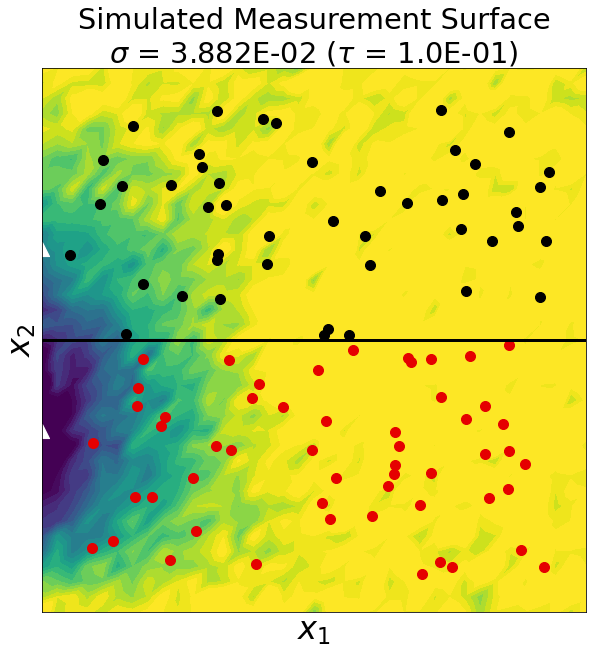
\includegraphics[width=0.5\linewidth]{figures/pde-highd/pde-highd_sensors_D2.png}
% \caption{
% A representative noisy perturbation of the reference response surface. Locations of the randomly chosen spatial data used to construct both $Q_{1D}$ and $Q_{2D}$ are shown as black and red dots.
% }
\label{fig:pde-Q}
\end{figure}
\end{frame}


%%%%%%%%%%%%%%%%%%%%%%%%%%%%%%%%%%%%%%%%%%%%%%%%%%%%%%%%%%%
\begin{frame}
\begin{figure}
\centering
\only<1>{
    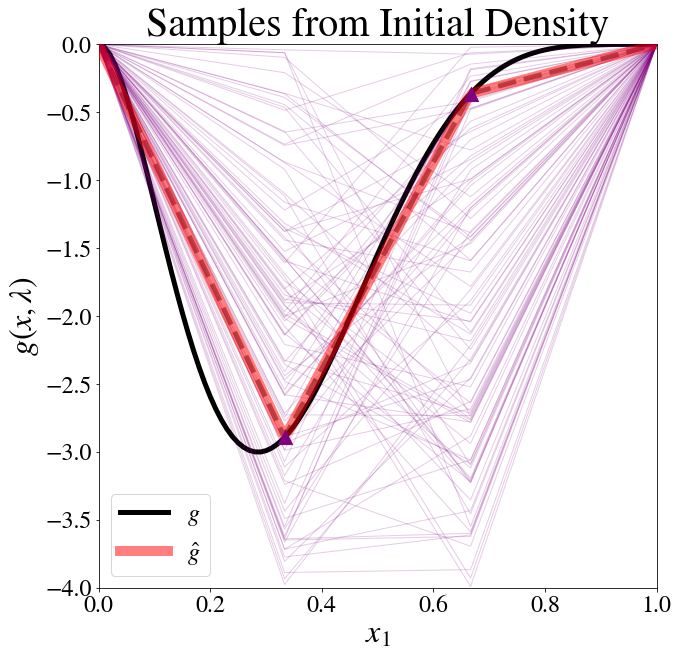
\includegraphics[width=0.7\linewidth]{figures/pde-highd/pde-highd_init_D2.png}
}
\only<2>{
		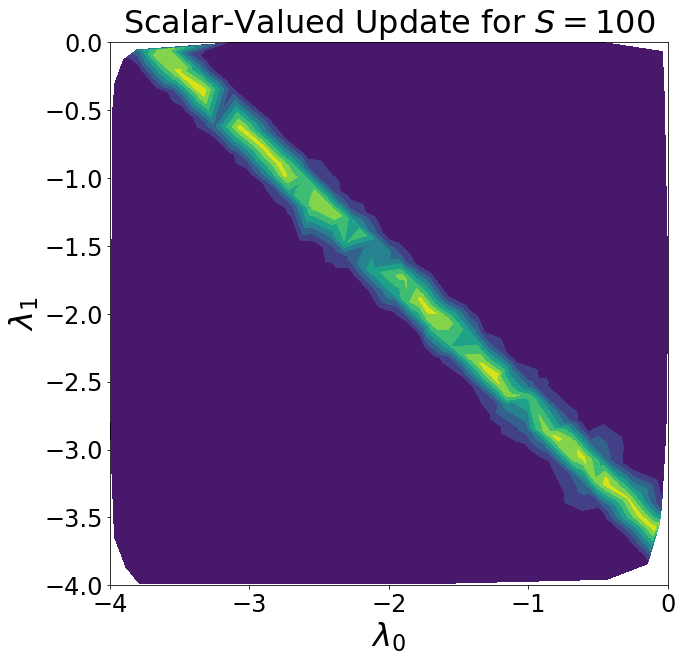
\includegraphics[width=0.35\linewidth]{figures/pde-highd/pde-highd_updated_D2_scalar.png}
		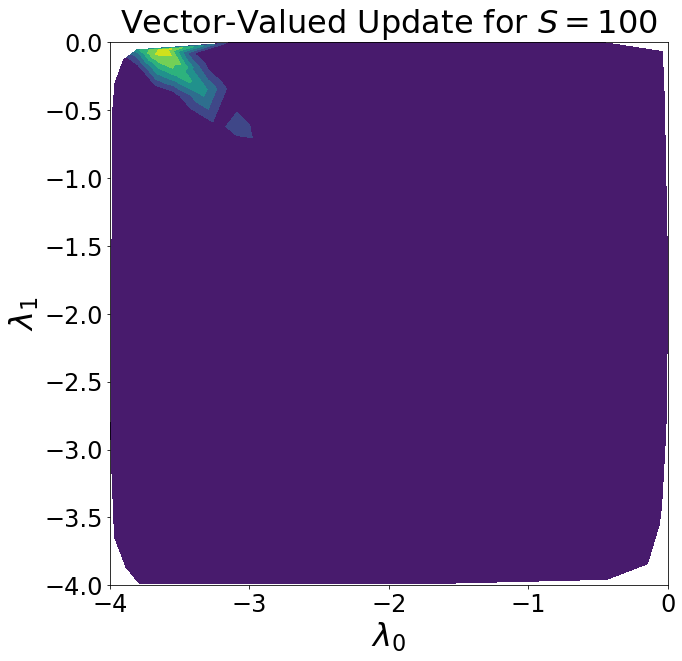
\includegraphics[width=0.35\linewidth]{figures/pde-highd/pde-highd_updated_D2_vector.png}
		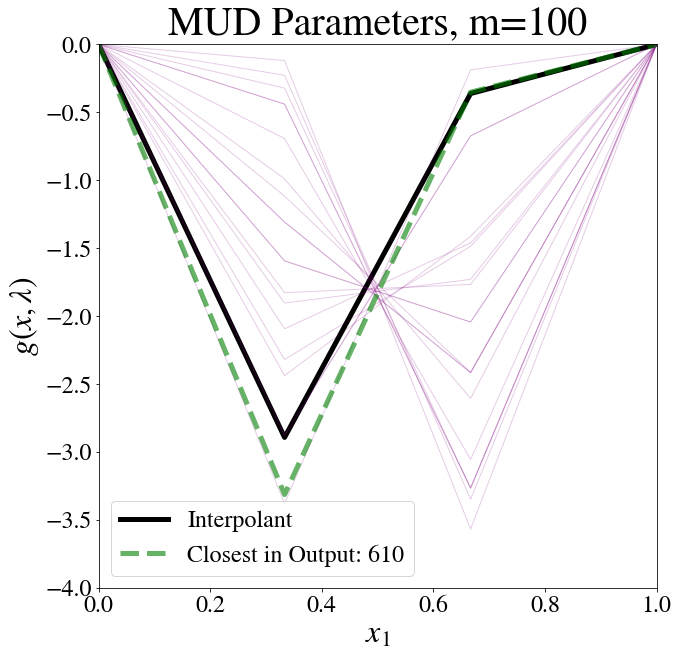
\includegraphics[width=0.35\linewidth]{figures/pde-highd/pde-highd_pair_D2-1_m100.png}
		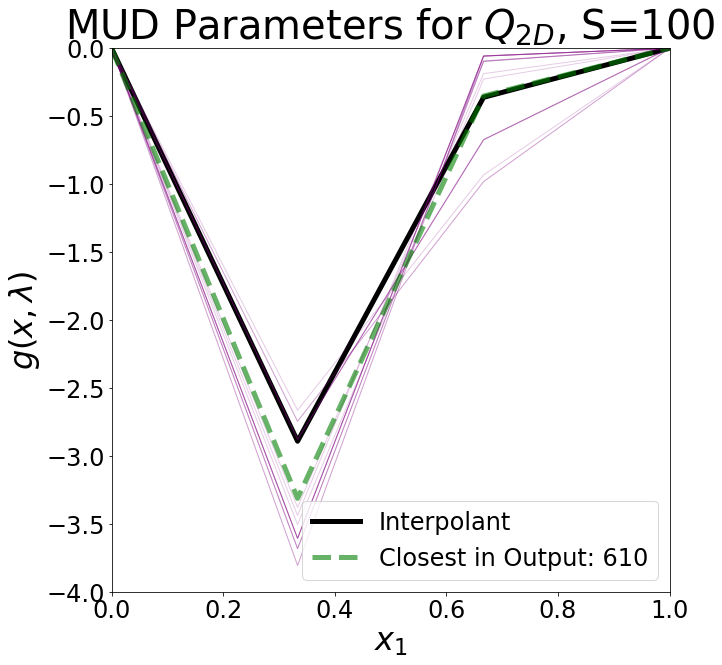
\includegraphics[width=0.35\linewidth]{figures/pde-highd/pde-highd_pair_D2-2_m100.png}

}
% \caption{
% In the left plot, the reference $g(x_2)$ is shown as the solid black curve with its interpolant onto the spline basis shown as a dotted red curve.
% The dashed blue line represents the sample from parameter space which most closely predicts noiseless data, which we refer to as the projection of $g$.
% The purple curves in the center and right plots show the variability in MUD estimates of $g(x_2)$ for the 20 different realizations of noisy data.
% The center plot uses $Q_{1D}$ and the right plot uses $Q_{2D}$ to construct the MUD estimates.
% }
\label{fig:pde-MUD}
\end{figure}
\end{frame}

%%%%%%%%%%%%%%%%%%%%%%%%%%%%%%%%%%%%%%%%%%%%%%%%%%%%%%%%%%%
%%%%%%%%%%%%%%%%%%%%%%%%%%%%%%%%%%%%%%%%%%%%%%%%%%%%%%%%%%%
\section{Extensions and Future Work}
%%%%%%%%%%%%%%%%%%%%%%%%%%%%%%%%%%%%%%%%%%%%%%%%%%%%%%%%%%%
%%%%%%%%%%%%%%%%%%%%%%%%%%%%%%%%%%%%%%%%%%%%%%%%%%%%%%%%%%%


%%%%%%%%%%%%%%%%%%%%%%%%%%%%%%%%%%%%%%%%%%%%%%%%%%%%%%%%%%%
\subsection{Geometry Makes a Comeback}
%%%%%%%%%%%%%%%%%%%%%%%%%%%%%%%%%%%%%%%%%%%%%%%%%%%%%%%%%%%

\begin{frame}[t]

\begin{figure}
\centering
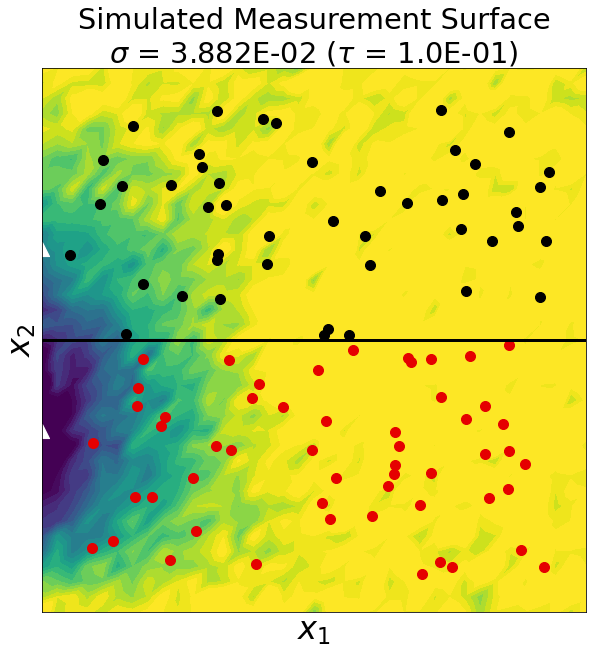
\includegraphics[width=0.25\linewidth]{figures/pde-highd/pde-highd_sensors_D2.png}
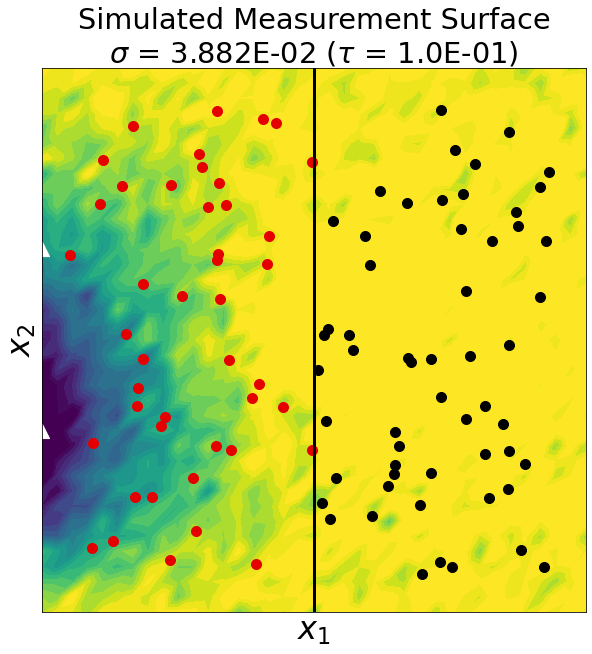
\includegraphics[width=0.25\linewidth]{figures/pde-highd/pde-highd_sensors-alt_D2.png}
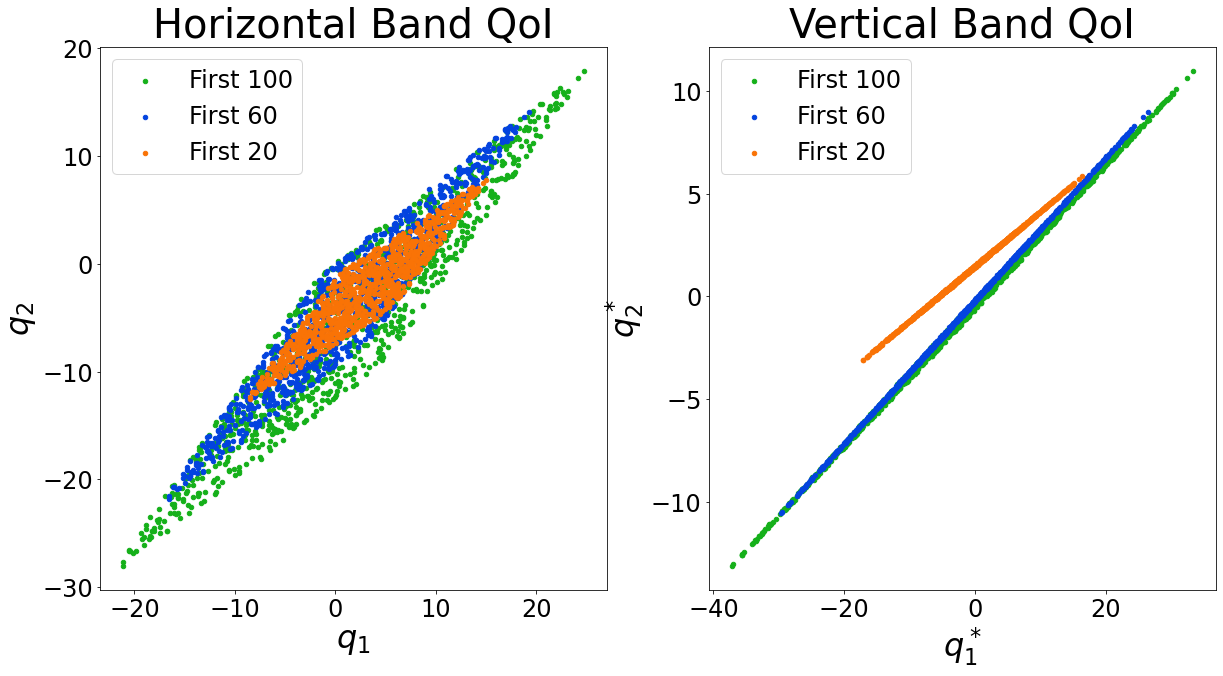
\includegraphics[width=0.5\linewidth]{figures/pde-highd/pde-highd_geom_D2.png}
% \caption{
% $N=1000$ parameter evaluations for both methods of partitioning $\Omega$.
% }
\label{fig:pde-highd-2d-geometry}
\end{figure}

\end{frame}


%%%%%%%%%%%%%%%%%%%%%%%%%%%%%%%%%%%%%%%%%%%%%%%%%%%%%%%%%%%
\begin{frame}[t]

\begin{figure}
  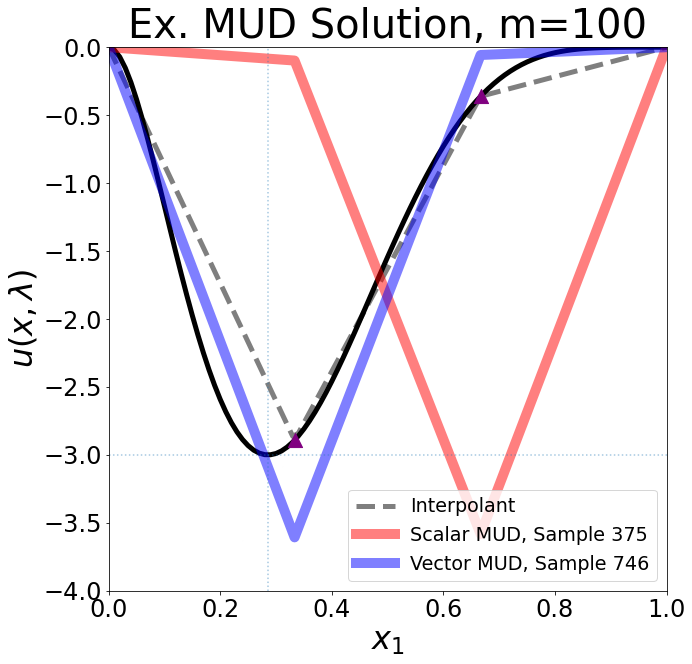
\includegraphics[width=0.95\linewidth]{figures/pde-highd/pde-highd_comp_exmud_D2_m100.png}
% \caption{
% Side-by-side comparison of an example solution to the SIP using $\qoi_\text{1D}$ (left) compared to using $\qoi_\text{2D}^\prime$, juxtaposed against a plot of $g$.
% }
\label{fig:pde-highd-2d-scalar-vs-alt}
\end{figure}

\end{frame}


%%%%%%%%%%%%%%%%%%%%%%%%%%%%%%%%%%%%%%%%%%%%%%%%%%%%%%%%%%%n
\subsection{Iterating}
%%%%%%%%%%%%%%%%%%%%%%%%%%%%%%%%%%%%%%%%%%%%%%%%%%%%%%%%%%%

\begin{frame}[t]

The one with the small problems in many batches.

QoI defined by $10$ equispaced rotations of the unit vector $[0, 1]$ through the first two Euclidean quadrants

\begin{figure}
  \centering
  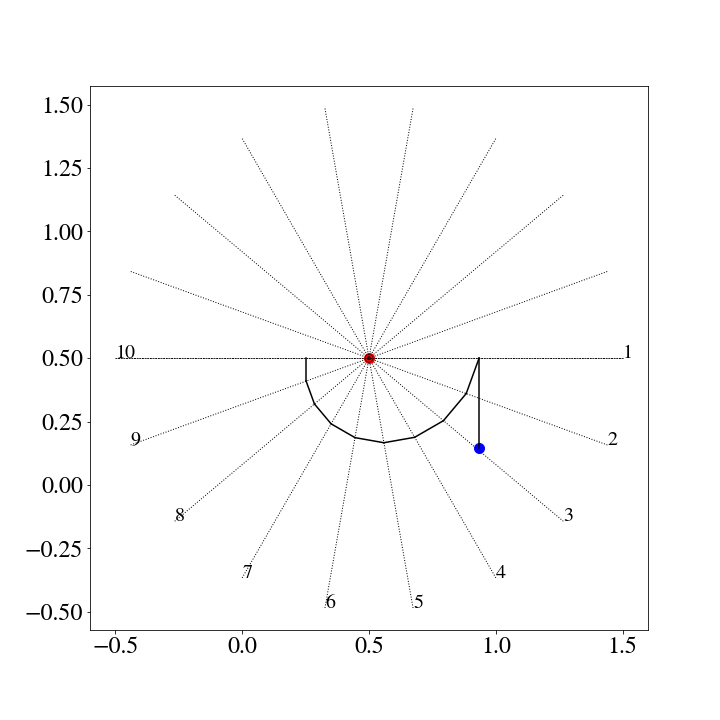
\includegraphics[width=0.475\linewidth]{figures/iterative/10D-firstepoch.png}
  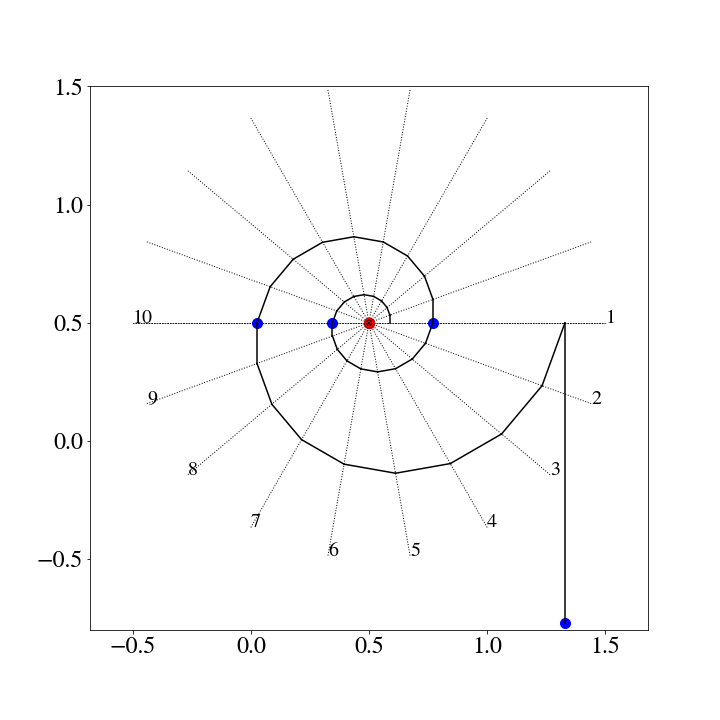
\includegraphics[width=0.475\linewidth]{figures/iterative/10D-fewepochs.png}
  % \caption{
  % Dotted lines show the solution contours for each row of the operator $A$.
  % (Left): First epoch for iterating through 10 QoI.
  % (Right): Three more epochs allows our estimate to get much closer to the true value.
  % }
  \label{fig:iterative-linear-demo}
\end{figure}

\end{frame}

\begin{frame}[t]
%\vskip 25pt
\begin{figure}
\centering

\only<1>{
\begin{figure}
  \centering
  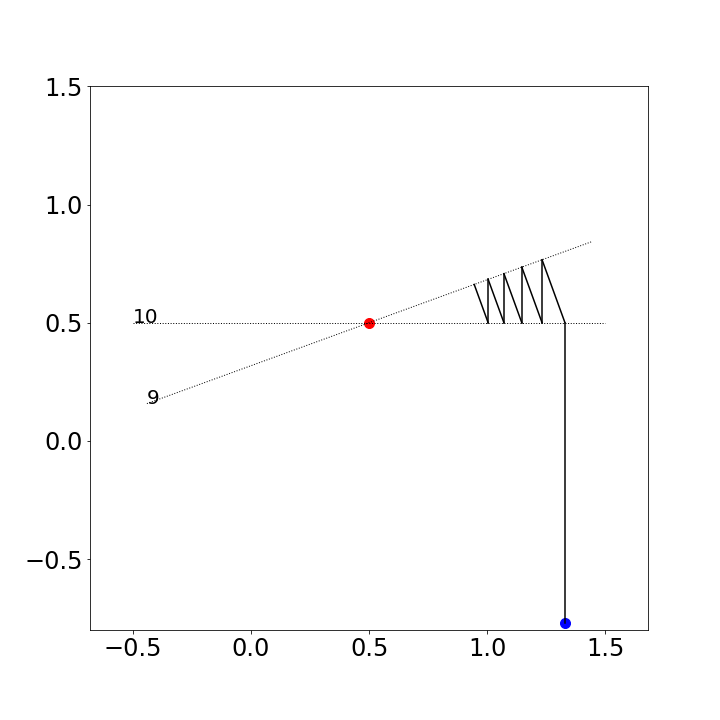
\includegraphics[width=0.475\linewidth]{figures/iterative/10D-fewepochs-pair.png}
  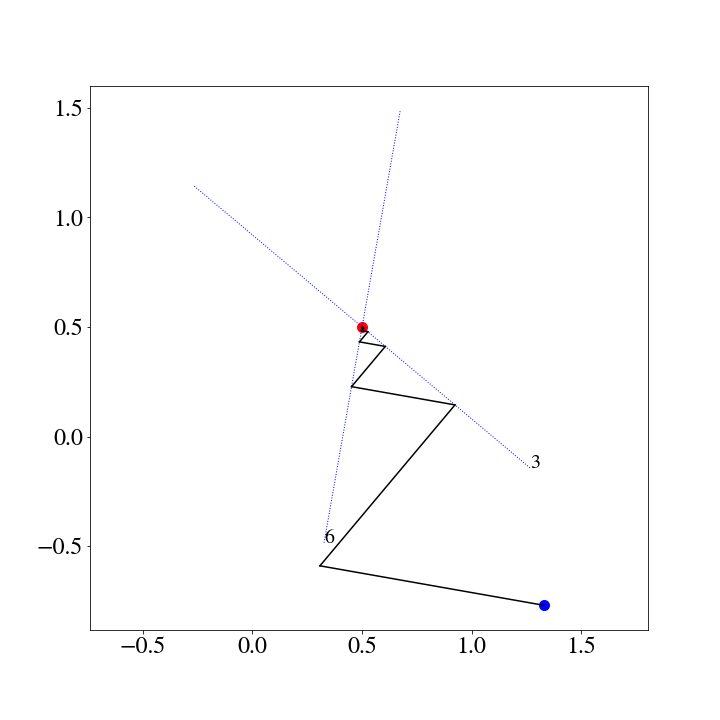
\includegraphics[width=0.475\linewidth]{figures/iterative/10D-fewepochs-pair-alt.png}
  % \caption{
  % Iterating through five epochs of two QoI, each formed by picking two of the ten available rows of $A$ at random.
  % The random directions chosen on the left exhibit more redundancy than those on the right, so the same amount of iteration results in less accuracy.
  % }
  \label{fig:iterative-linear-demo-pair}
\end{figure}
}

\only<2>{
\begin{figure}
  \centering
  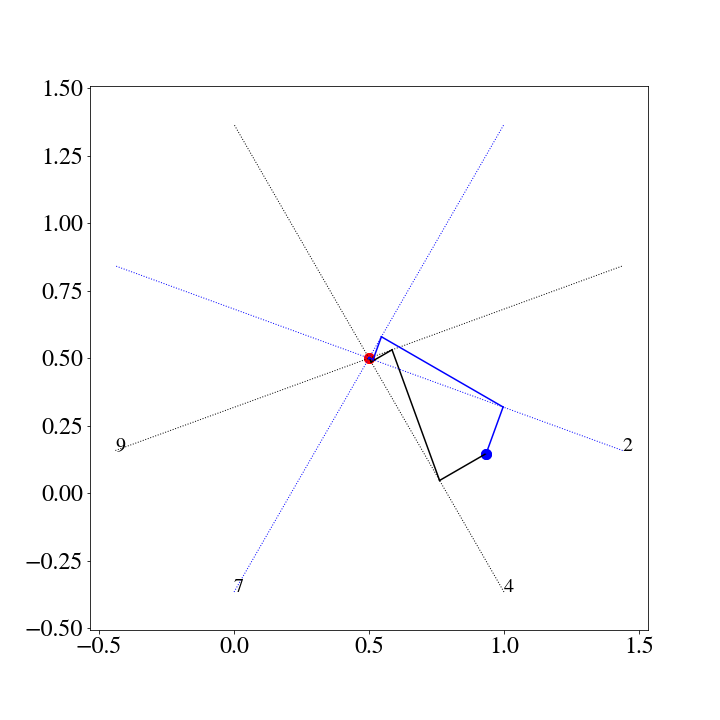
\includegraphics[width=0.475\linewidth]{figures/iterative/10D-firstepoch-pair-smart.png}
  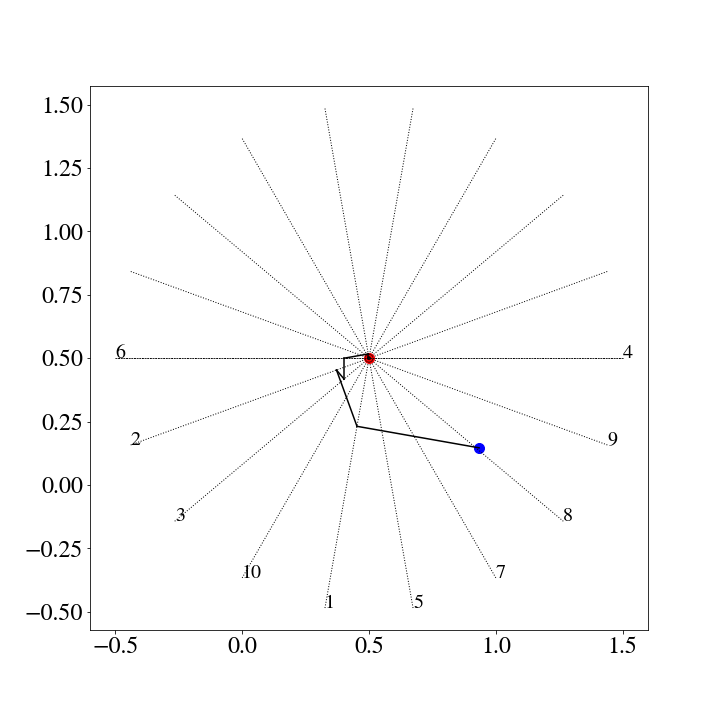
\includegraphics[width=0.475\linewidth]{figures/iterative/10D-firstepoch-rand.png}
  % \caption{
  % (Left): Subsets of available QoI components can be chosen to exhibit minimal redudancy and lead to expedited convergence.
  % (Right): Random components of the QoI map used for each iterative step. This leads to an overall similar level of precision in this example, without the need to use gradients.
  % }
  \label{fig:iterative-linear-demo-smart}
\end{figure}
}

\only<3>{
\begin{figure}
  \centering
  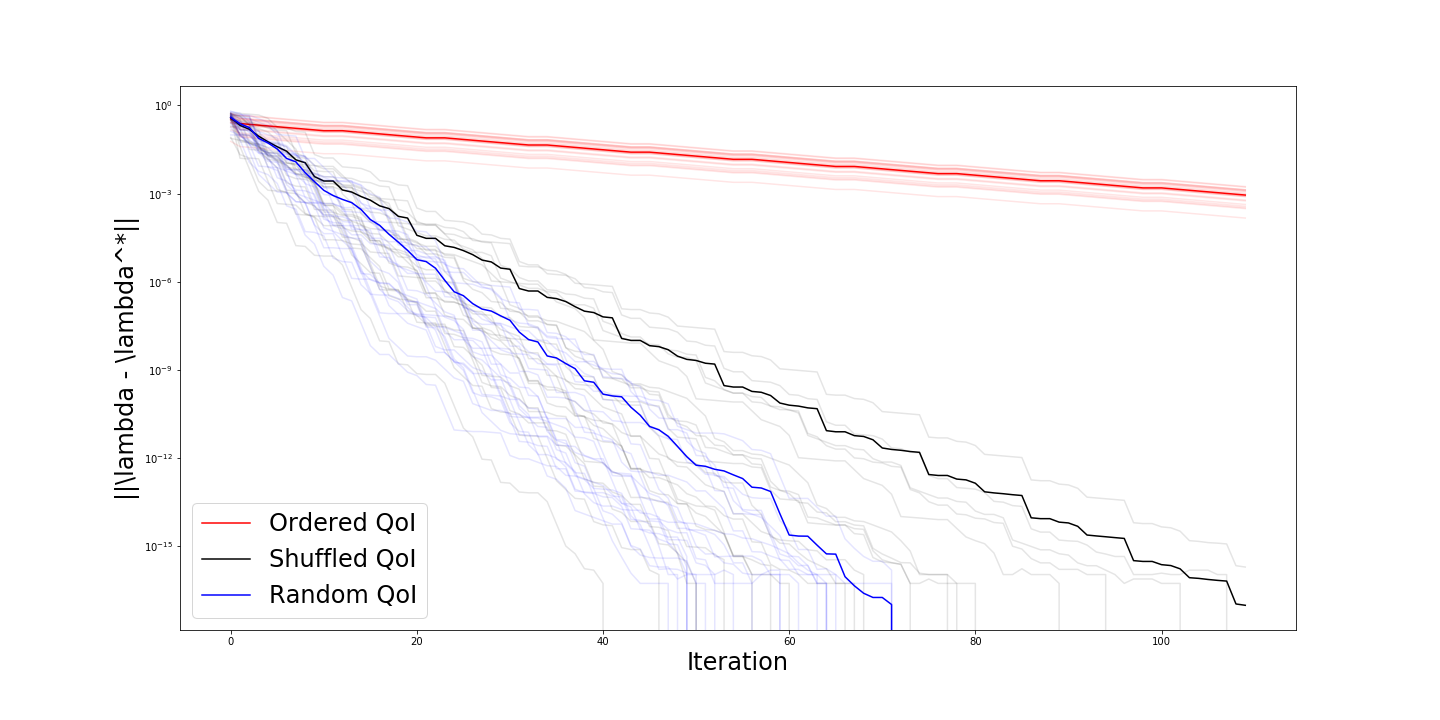
\includegraphics[width=0.95\linewidth]{figures/iterative/10D-convergence-comparison.png}
  % \caption{
  % 20 initial means are chosen and iterated on for three approaches for ordering QoI.
  % Individual experiments are transparent and the mean error is shown as a solid line for each approach.
  % }
  \label{fig:iterative-convergence-comparison}
\end{figure}
}


\end{figure}
\end{frame}


%%%%%%%%%%%%%%%%%%%%%%%%%%%%%%%%%%%%%%%%%%%%%%%%%%%%%%%%%%%
\subsection{Software}
%%%%%%%%%%%%%%%%%%%%%%%%%%%%%%%%%%%%%%%%%%%%%%%%%%%%%%%%%%%

\begin{frame}[t]{\it The one where we convince you to trust our numerics.}
%\vskip 25pt
\centering
\begin{figure}
\begin{itemize}
	\item Public repository hosted on Github.com ({\tt github.com/mathematicalmichael/thesis})
	\item Github Actions implements Continuous Integration / Deployment
	\item Each change is validated for reproducibility
	\item {\tt makefile} for convenience ({\tt make <filename>})
	\begin{itemize}
		\item dissertation + presentation (\LaTeX, themes, style files)
		\item every example, convergence result (Python)
		\item every image in every figure
	\end{itemize}
	\item PyPi published implementation of main methods: {\tt pip install mud}
	\item Unit tests aid in ensuring integrity of functions
	\item Docker guarantees software runtime (ran on {\tt x86} and {\tt arm}) \\ {\tt docker pull mathematicalmichael/python:thesis}({\tt latex:thesis})
\end{itemize}

\end{figure}

\end{frame}



% %%%%%%%%%%%%%%%%%%%%%%%%%%%%%%%%%%%%%%%%%%%%%%%%%%%%%%%%%%%%%%%%%%%%
%%%%%%%%%%%%%%%%%%%%%%%%%%%%%%%%%%%%%%%%%%%%%%%%%%%%%%%%%%%%%%%%%%%%
\section{Comparing Inverse Problems and Solutions}\label{sec:compare}
%%%%%%%%%%%%%%%%%%%%%%%%%%%%%%%%%%%%%%%%%%%%%%%%%%%%%%%%%%%%%%%%%%%%
%%%%%%%%%%%%%%%%%%%%%%%%%%%%%%%%%%%%%%%%%%%%%%%%%%%%%%%%%%%%%%%%%%%%
It is important to note that the Bayesian framework poses a different question for which a different answer is sought.
Specifically, the problem analyzed by the Bayesian approach is to determine a single ``true'' parameter that explains all of the observed data \cite{Smith, Concrete, Complete}.
The philosophical underpinnings of Bayesian inference is akin to the asking following:

\begin{center}
  \emph{How does one incorporate collected data to shift prior beliefs about specific parameter values?}
\end{center}

The philosophical underpinnings of Bayesian inference are distinct from the Data-Consistent framework, where we seek a pull-back measure: a description of the uncertainty set that explains the variation in the observations under a given description of error.
This approach expresses a desire to reconstruct a distribution (or probability measure), asking:

\begin{center}
  \emph{How does one update prior beliefs in such a way that modifies predictions to match the description of uncertainty in observed data?}
\end{center}


\subsubsection{The Bayesian inverse problem}

We now develop a typical Bayesian inverse problem following the framework described in \cite{Stuart10}.
Let $d$ denote the ``noisy'' data obtained on $Q(\paramref)$, which is often represented as
\begin{equation*}
	d = Q(\paramref) + \xi,
\end{equation*}
where $\xi$ is a random variable used to model the measurement error that is often assumed to follow a Gaussian distribution.
Then, the data-likelihood function, often written as a conditional density, $L_\dspace(\q)\, |\, \param)$, is formed.
This describes the differences in relative likelihoods that the data could have been generated from a particular $\param$.
Ideally, the largest values of $L_\dspace(\q)\, | \, \param)$ occur whenever $\param$ is a ``good'' approximation to the true parameter $\paramref$.
The data-likelihood function is distinct from the observed density used in the observation-consistent framework.

The next ingredient in the Bayesian framework is the specification of a prior density denoted by $\pi_\text{prior}(\param)$.
The prior describes the different relative likelihoods assumed for the true parameter before data are collected.
This is also distinct from the role of the {\em initial} density used in the observation-consistent framework.
We choose them to represent the set of feasible parameters, and rely on Monte-Carlo sampling for both approaches\footnote{Priors in Bayesian inference are sometimes chosen for reasons related to Markov-Chain Monte-Carlo algorithms in order to ensure their balancing of investigation and exploration, or convergence [TK - cite someone]}.

The posterior density (i.e., the solution to the Bayesian inverse problem) is given by a conditional density, denoted by $\pi_\text{post}(\param\, | \, d)$, proportional to the product of the prior and data-likelihood function.
In other words,
\begin{equation*}
	\posterior(\param\, | \, \q) \propto \prior(\param)L_\dspace(\q\, | \, \param)
\end{equation*}
This form of the density follows from Bayes' rule (not from the Disintegration Theorem as with the updated density).
The posterior can be interrogated to assess the difference in relative likelihoods of a fixed parameter given the observed data.
Subsequently, the posterior is often used to produce a ``best'' estimate of the true parameter.
For example, the maximum a posteriori (MAP) point is the parameter that maximizes the posterior density.

The Bayesian formulation \citep{Walpole, Berger, Complete, Smith} gives a posterior density as:

\begin{equation}\label{eq:sb_post}
    \posterior\lam := \prior\lam \frac{L_\dspace (\q | \param)}{ C },
\end{equation}

where we use $\posterior$ to distinguish the \emph{posterior} from the updated density $\updated$ in \eqref{eq:update}.


$L_\dspace$ is the likelihood function as a function of the output and the denominator $C$ is a normalizing constant (known as the \emph{evidence} \cite{Smith}), which ensures the posterior density integrates to one:
\[
C = \int_\pspace \prior\lam L_\dspace(\q | \param) \, d\param.
\]

Note that there are no constraints or requirements that likelihood function be a density.
In fact, $L_\dspace$ need not even be in $L^1(\pspace)$ since it is actually only the product $\prior(\param) L_\dspace (\q | \param)$ that is required to be in $L^1(\pspace)$ to form a posterior.
In other words, $L_\dspace (\q | \param)$ and $\observed(\q)$ can model completely different things with respect to uncertainty in the data.
An interpretation of $L_\dspace (\q | \param)$ is the relative likelihood that a single parameter $\param\in\pspace$ explains the observed data, whereas $\observed(\q)$ describes the relative likelihood of a predicted datum associated with $\param\in\pspace$.
In this framework, there is a different notion of consistency, referring to certain asymptotic properties of $\posterior$ in the limit of infinite data \cite{Barron, Silverman}.



%%%%%%%%%

\subsection{Comparison to Bayesian Inversion}\label{sec:bayesian}

We summarize the posterior and updated densities side-by-side in Table~\ref{tab:dens_comparisons} and comment on a few notable aspects not mentioned above.
Observe for the posterior density that the data-likelihood function appears in both the numerator and denominator.
In particular, the data-likelihood function informs the {normalizing constant}, commonly referred to as the evidence term, in the denominator.
This is in contrast to the denominator of the updated density, which is given by the predicted density, which is in general not a constant, and can be constructed independently of $\observed$

\begin{table}[htbp]
\centering
\begin{tabular}{|c|c|}
\hline
 & \\
$\displaystyle \updated(\param) = \initial(\param) \frac{\observed(\q)}{\predicted(\q)}
$
&
$
	\displaystyle \pi_{\text{post}}(\param\,|\,\q) = \frac{\prior(\param)L_\dspace(\q)\,|\,\param)}{\int_{\Lambda} L_\dspace(\q)\, |\, \param)  \prior(\param) d\pmeas}
$
 \\ & \\ \hline
\end{tabular}
\caption{Updated density solving the observation-consistent inverse problem (left) and posterior density solving the Bayesian inverse problem (right).}
		\label{tab:dens_comparisons}
\end{table}

A practical implication of this difference is that the updated density only alters the structure of the initial density in what we refer to as the ``data-informed'' parameter directions.
Specifically, for a fixed $\q\in\dspace$, let $C_\q := \set{\param\in\pspace\, : \, \qlam=\q}$, i.e., $C_\q$ is a ``contour'' in parameter space.
Then, for any $\param\in C_\q$, we immediately have $\updated(\param)=r(\q)\initial(\param)$ where $r(\q)$ is a fixed constant of proportionality for all $\param\in C_\q$.
%Subsequently, using the Disintegration theorem on both the initial and updated densities produces exactly the same family of conditional densities on the contours in parameter space.
By contrast, while the posterior does not have to agree with the prior in any direction in parameter space, the prior does impact the structure of the posterior in all directions.

The previous paragraph is not\---and should not be interpreted as\---a criticism of the Bayesian inverse framework.
It is simply meant to highlight that the observation-consistent and Bayesian frameworks formulate and solve inverse UQ problems from different perspectives and with different (although at times seemingly compatible) assumptions.
Consequently, the solutions for an inverse problem formulated under either framework may differ significantly.
As the example (adopted from \cite{BJW18}) below demonstrates, this is true even if we arbitrarily force the inverse problems to appear as similar as possible.
\vfill

% 
\section{Research Questions}
%%%%%%%%%%%%%%%%%%%%%%%%%%%%%%%%%%%%%%%%%%%%%%%%%%%%%%%%%%
\begin{frame}[t]
\begin{itemize}
	\item In the explicit approach, a finite numerical approximation of (often uncountably many) events in $\sa$s is required.
	\item Two primary sources of approximation error: 
	\begin{itemize}
	
		\item (1) partitioning the parameter space $\pspace$ to approximate events in $\pborel$
		\item (2) partitioning the data space $\dspace$ to approximate events in $\BBB_{\dspace}$
	
	\end{itemize}
	\item A non-intrusive sample-based algorithm is initially introduced in \cite{BET+14} and further analyzed in \cite{BET+14-arxiv}
\end{itemize}
\end{frame}


%%%%%%%%%%%%%%%%%%%%%%%%%%%%%%%%%%%%%%%%%%%%%%%%%%%%%%%%%%
\begin{frame}[t]
\begin{itemize}
	\item <1-> Let $\predictedPxM$ be the exact solution to the approximate inverse problem using the discretization of $P_\dspace$ by $M$ samples
	\item <2-> Let $\predictedPxNM$ denote the approximate solution to the approximate problem under both aforementioned discretizations, so 
\[
\predictedP = \lim\limits_{M\to\infty} \predictedPxM = \lim\limits_{M\to\infty} \lim\limits_{N\to\infty} \predictedPxNM
\]
	\item <3-> Let $\predictedPxNMh$ denote the approximate solution given the model discrepancy
\[
\predictedPxNM= \lim\limits_{h \downarrow 0} \predictedPxNMh
\]
\item <3-> $h$ refers to a mesh or other numerical parameter that determines the accuracy of the numerical solution evaluation of the QoI map
\end{itemize}

\end{frame}

%%%%%%%%%%%%%%%%%%%%%%%%%%%%%%%%%%%%%%%%%%%%%%%%%%%%%%%%%%
\begin{frame}[t]

Repeated application of the triangle inequality yields
\begin{equation}
\label{eq:triangleineq}
d_{\text{TV}}(\predictedPxNMh, \predictedP) \leq 
\underset{ \text{(E1)} }{\underbrace{ d_{\text{TV}}(\predictedPxNMh, \predictedPxNM)}} + 
\underset{ \text{(E2)} }{\underbrace{ d_{\text{TV}}(\predictedPxNM, \predictedPxM) }}+ 
\underset{ \text{(E3)} }{\underbrace{ d_{\text{TV}}(\predictedPxM, \predictedP) }}.
\end{equation}
\begin{itemize}

	\item <1-> The term (E1) describes the effect of the error in the numerically evaluated $Q_j$ on the solution to the stochastic inverse problem
	\item <2-> The term (E2) describes the effect of finite sampling error in $\pspace$, and (E3) describes the effect of discretization error of $P_\dspace$ on the solution to the stochastic inverse problem
	\item <3-> In our experience, terms (E1) and (E3) are more easily controlled
	\item <3-> Limit our focus to (E2), where certain geometric properties of the QoI map have an impact
\end{itemize}
\end{frame}

\subsection{Skewness and Accuracy}
%%%%%%%%%%%%%%%%%%%%%%%%%%%%%%%%%%%%%%%%%%%%%%%%%%%%%%%%%%
\begin{frame}[t]
\begin{itemize}
	\item In \cite{BGE+15}, the concept of \emph{skewness} in a QoI map $Q$ is introduced, quantified, and related to the accuracy in solving the stochastic inverse problem with a finite number of samples
	\item Geometric property that describes how the right angles in generalized rectangles belonging to $\dborel$ are transformed by $Q^{-1}$
\end{itemize}

\begin{defn}
For any QoI map $Q$, $\lambda \in \pspace$, and row vector $\bf{j}_k$ of Jacobian $J_{\lambda, Q}$, we define
\begin{equation}
S_Q(J_{\lambda,Q}, \bf{j}_k) := \frac{\abs{\bf{j}_k} }{\abs{\bf{j}_k^\perp}}.
\label{eq:skewness}
\end{equation}
We define the \textbf{local skewness} of a map $Q$ at a point $\pspace$ as 
\begin{equation}
S_Q(\lambda) := \max_{1\leq k \leq d} S_Q(J_{\lambda,Q}, \bf{j}_k).
\label{eq:localskewness}
\end{equation}
\end{defn}

\end{frame}

%%%%%%%%%%%%%%%%%%%%%%%%%%%%%%%%%%%%%%%%%%%%%%%%%%%%%%%%%%
\begin{frame}[t]
\begin{defn}
For any QoI map $Q$, $\lambda \in \pspace$, and row vector $\bf{j}_k$ of Jacobian $J_{\lambda, Q}$, we define
\begin{equation}
\begin{split}
S_Q(J_{\lambda,Q}, \bf{j}_k) &:= \frac{\abs{\bf{j}_k} }{\abs{\bf{j}_k^\perp}} \\
S_Q(\lambda) &:= \max_{1\leq k \leq d} S_Q(J_{\lambda,Q}, \bf{j}_k)
\end{split}
\end{equation}
\end{defn}

\begin{defn}
The \textbf{average} \emph{(or \textbf{expected})} \textbf{skewness} is defined as
\begin{equation}
\overline{S_Q} := \frac{1}{\mu_{\pspace}(\pspace)} \int_\pspace S_Q (\lambda) \, d\mu_{\pspace}
\label{eq:avgskew}
\end{equation}
\end{defn}

\begin{itemize}
	\item In \cite{BPW17}, it is shown that $S_Q(\lambda)$ is efficiently computed using SVDs of the Jacobian $J_{\lambda,Q}$
	\item In general, we approximate $\overline{S_Q}$ with Monte-Carlo approximations
\end{itemize}

\end{frame}




%%%%%%%%%%%%%%%%%%%%%%%%%%%%%%%%%%%%%%%%%%%%%%%%%%%%%%%%%%


%%%%%%%%%%%%%%%%%%%%%%%%%%%%%%%%%%%%%%%%%%%%%%%%%%%%%%%%%%
\begin{frame}[t]{A Simple Example: The Identity Map}
\vspace{-10pt}
\begin{figure}
	\begin{minipage}{.3\textwidth}
		\begin{itemize}
			\item $50$ samples
			\vskip 60pt
			\item $200$ samples
			\vskip 60pt
			\item $3200$ samples
		\end{itemize}
	\end{minipage}
	\begin{minipage}{.55\textwidth}
		\centering
    		$\Lambda$ \hskip 80pt $\mathcal{D}$
    		\vskip 0pt
    		\includegraphics[width=.5\textwidth]{images/finitesampling/approximate_input_50}
			\includegraphics[width=.5\textwidth]{images/finitesampling/approximate_output_50}\\
		\includegraphics[width=.5\textwidth]{images/finitesampling/approximate_input_200}
			\includegraphics[width=.5\textwidth]{images/finitesampling/approximate_output_200}\\
		\includegraphics[width=.5\textwidth]{images/finitesampling/approximate_input_3200}
			\includegraphics[width=.5\textwidth]{images/finitesampling/approximate_output_3200}\\
	\end{minipage}
\end{figure}

\end{frame}


%%%%%%%%%%%%%%%%%%%%%%%%%%%%%%%%%%%%%%%%%%%%%%%%%%%%%%%%%%
\begin{frame}[t]{Skewness}

\begin{figure}
    \begin{minipage}{.5\textwidth}
    	\centering
    	$\Lambda$
    	\vskip 0pt
    	\includegraphics[width=1\textwidth]{images/samemeasure_orthog}\\
    	\vskip 0pt
        %$\mu_\Lambda((Q^{(a)})^{-1}(B^{(a)})) = 0.0769$
    \end{minipage}%
    \begin{minipage}{.5\textwidth}
    \centering
    	$\Lambda$
    	\vskip 0pt
    	\includegraphics[width=1\textwidth]{images/samemeasure_skew}
        \vskip 0pt
    	%$\mu_\Lambda((Q^{(b)})^{-1}(B^{(b)})) = 0.0769$
    \end{minipage}
\end{figure}


\end{frame}

%%%%%%%%%%%%%%%%%%%%%%%%%%%%%%%%%%%%%%%%%%%%%%%%%%%%%%%%%%
\begin{frame}[t]{Numerical Approximation | Skewness}
\vspace{-10pt}
\begin{figure}
	\begin{minipage}{.3\textwidth}
		\begin{itemize}
			\item $50$ samples
			\vskip 60pt
			\item $200$ samples
			\vskip 60pt
			\item $800$ samples
		\end{itemize}
	\end{minipage}
	\begin{minipage}{.55\textwidth}
		\centering
    		$\Lambda$ \hskip 80pt $\Lambda$
    		\vskip 0pt
    		\includegraphics[width=.5\textwidth]{images/finitesampling/voronoi_symmdiff_orthog_50samples}
			\includegraphics[width=.5\textwidth]{images/finitesampling/voronoi_symmdiff_skew_50samples}\\
		\includegraphics[width=.5\textwidth]{images/finitesampling/voronoi_symmdiff_orthog_200samples}
			\includegraphics[width=.5\textwidth]{images/finitesampling/voronoi_symmdiff_skew_200samples}\\
		\includegraphics[width=.5\textwidth]{images/finitesampling/voronoi_symmdiff_orthog_800samples}
			\includegraphics[width=.5\textwidth]{images/finitesampling/voronoi_symmdiff_skew_800samples}\\
	\end{minipage}
\end{figure}

\end{frame}

%%%%%%%%%%%%%%%%%%%%%%%%%%%%%%%%%%%%%%%%%%%%%%%%%%%%%%%%%%
\begin{frame}[t]
\begin{example}
\label{ex:skewness}
Consider the following family of linear maps:
\begin{equation}\label{eq:qmap2}
\left \lbrace Q^{(s)} =  \mat{cc}{1 & 0 \\ \sqrt{s^2 - 1}& 1 } \right \rbrace_{s\in S},
\end{equation}
for $S=\set{1,2,4}$. 
\begin{itemize}
	\item Designed so the skewness of these maps is given by the index $s$, so $Q^{(1)}$ is $1$, the skewness of $Q^{(2)}$ is $2$, and $S_{Q^{(4)}} = 4$
	\item Preserves sizes of sets (determinant is one)
	\item Skewness has a direct impact on the number of samples required to achieve a given accuracy
	\item Provided a strong motivation for minimizing skewness and reinforces the results from \cite{BPW_2015}
\end{itemize}
\end{example}

\end{frame}


%%%%%%%%%%%%%%%%%%%%%%%%%%%%%%%%%%%%%%%%%%%%%%%%%%%%%%%%%%
\begin{frame}[t]
\small
\begin{figure}[h]
\begin{table}[H]
\begin{tabular}{ c | c | c | c }

N & $Q^{(a)}$ & $Q^{(b)}$ & $Q^{(c)}$\\ \hline \hline
$200$ & $2.97E-01$ & $3.42E-01$ & $5.28E-01$\\ \hline

$400$ & $2.00E-01$ & $2.41E-01$ & $3.79E-01$\\ \hline

$800$ & $1.59E-01$ & $1.78E-01$ & $2.88E-01$\\ \hline

$1600$ & $1.06E-01$ & $1.31E-01$ & $1.93E-01$\\ \hline

$3200$ & $8.38E-02$ & $9.39E-02$ & $1.41E-01$\\ \hline

$6400$ & $6.14E-02$ & $6.40E-02$ & $1.05E-01$\\ \hline

\end{tabular}
\end{table}

		\includegraphics[width=0.5\linewidth]{./images/Plot-reg_BigN_40000_reg_M_1_rand_I_100000}

\caption{The results of $d_\text{TV}(\predictedPxNM, \predictedPxNN)$.}
\label{fig:skew}
\end{figure}
\end{frame}

%%%%%%%%%%%%%%%%%%%%%%%%%%%%%%%%%%%%%%%%%%%%%%%%%%%%%%%%%%
\subsection{Time Series Data}

%%%%%%%%%%%%%%%%%%%%%%%%%%%%%%%%%%%%%%%%%%%%%%%%%%%%%%%%%%
\begin{frame}[t]
\begin{itemize}
	\item Let $t_0$ denote the initial time for the system being modeled 
	\item Let $\set{t_i}_{i=1}^M$ denote a set of observation times such that $t_0\leq t_1<t_2<\ldots<t_M$
	\item For each $1\leq i\leq M$, let $d_i$ denote the (noisy) measured (scalar) datum associated with some observable model output
	\item For each $1\leq i\leq M$, let $O_i(\lambda)$ denote the predicted value for $d_i$ obtained by solving the model for a particular $\lambda\in\pspace$
	\item We make a standard assumption used in the literature \cite{Smith, Barron, Silverman, Walpole} of an additive error noise model with independent errors $\eta_i$ for each $1\leq i\leq M$, i.e.
	\begin{equation}\label{eq:obs_data_error}
	d_i = O_i(\lambda) + \eta_i, \ 1\leq i\leq M,
\end{equation}
	\item We make the additional assumption that $\eta_i\sim N(0,\sigma_i^2)$ for each $1\leq i\leq M$.
\end{itemize}


\end{frame}

%%%%%%%%%%%%%%%%%%%%%%%%%%%%%%%%%%%%%%%%%%%%%%%%%%%%%%%%%%

%%%%%%%%%%%%%%%%%%%%%%%%%%%%%%%%%%%%%%%%%%%%%%%%%%%%%%%%%%
\begin{frame}[t]{Fundamental Questions}
\begin{itemize}
	\item How do we construct a QoI map that incorporates all these observations?
	\item Should we treat observations as individual QoI in a vector-valued map or should we define a scalar-valued QoI map that incorporates all of the observations?
	\item Choosing a vector-valued approach will certainly introduce skewness effects into the QoI map, but doing this in an ``optimal'' way can reduce uncertainty~\cite{Walsh}.
	\item Choosing a scalar-valued approach that combines information across multiple observations will avoid skewness 
	\item Potentially at the cost of reducing the influence of potentially informative or sensitive observations on the posterior.
	\item Are some observations are more useful than others?
	\item Quantify utility of including less useful observations in the definition of the QoI map.
\end{itemize}

\end{frame}

%%%%%%%%%%%%%%%%%%%%%%%%%%%%%%%%%%%%%%%%%%%%%%%%%%%%%%%%%%
\subsection{Optimal Experimental Design - Questions and Considerations}
%%%%%%%%%%%%%%%%%%%%%%%%%%%%%%%%%%%%%%%%%%%%%%%%%%%%%%%%%%
\begin{frame}[t]
\begin{itemize}
	\item <1-> \emph{Quality of Measurements} -- Equipment with which we perform measurements introduces errors into the collected data.
	
	\item <2-> \emph{Duration of Experiment} -- Budgetary constraints, permits, access to equipment or space, and a host of other factors can influence the length of a given trial or experiment.
	
	\item <3-> \emph{Number of Trials} -- Can we achieve accuracy with fewer repetitions of an experiment?
	
	\item <4-> \emph{Measurement Frequency} -- How many measurements to take in each trial is directly related to the potential savings of shortening an experiment or reducing the number of repetitions necessary. 
	\item <4-> Is it better to temporally compress a fixed number of observations or space them out? 
	
	\item <5-> Can we potentially conduct shorter experiments that are equally informative to save time?
	\item <5-> Is it worth investing in something that is faster but less accurate? What are the trade-offs for precision and accuracy in the posterior?	
\end{itemize}

\end{frame}


%%%%%%%%%%%%%%%%%%%%%%%%%%%%%%%%%%%%%%%%%%%%%%%%%%%%%%%%%%
\begin{frame}[t]{Some More Considerations}
\begin{itemize}
	\item Current computational bottleneck is memory transfer and storage rather than processing speed.
	\item Questions of how to sift through data and pick out the most informative subsets of critical relevance to many scientists.
	\item If data are already collected, research is needed with respect to defining a QoI.
	\item There is a need for numerical studies investigating how information gain changes as more data are utilized.
	\item Subject of future investigation?
\end{itemize}
\end{frame}


% conclude presentation
%%%%%%%%%%%%%%%%%%%%%%%%%%%%%%%%%%%%%%%%%%%%%%%%%%%%%%%%%%
% \begin{frame}[t]{}
% \vskip 64pt
% \begin{center}
% \Huge Thank You
% \end{center}
% \end{frame}
%%%%%%%%%%%%%%%%%%%%%%%%%%%%%%%%%%%%%%%%%%%%%%%%%%%%%%%%%%

\bibliographystyle{plain}
\bibliography{references.bib}





%%%%%%%%%%%%%%%%%%%%%%%%%%%%%%%%%%%%%%%%%%%%%%%%%%%%%%%%%%
%%%%%%%%%%%%%%%%%%%%%%%%%%%%%%%%%%%%%%%%%%%%%%%%%%%%%%%%%%
%%%%%%%%%%%%%%%%%%%%%%%%%%%%%%%%%%%%%%%%%%%%%%%%%%%%%%%%%%



\end{document}
